
\clearpage
\section{Background Study}
\label{sec:bkg_stu}
In the study of background processes, the main backgrounds are categorized into $e^{+}e^{-} \to \pi^{+}\pi^{-}\pi^{0}\pi^{0}$, $e^{+}e^{-} \to \pi^{+}\pi^{-}\pi^{0}\pi^{0}\gamma_{\text{ISR}}$, QED processes, and others. The dominant contributions arise from processes with additional $\pi^{0}$, particularly $e^{+}e^{-} \to \pi^{+}\pi^{-}\pi^{0}\pi^{0}$, while $e^{+}e^{-} \to \pi^{+}\pi^{-}\pi^{0}\pi^{0}\gamma_{\text{ISR}}$ is not dominant but shares the same underlying mechanism as a background to our signal. In the inclusive analysis, the cross sections used for these two processes were not correctly configured.

To verify that these processes constitute the primary backgrounds, the
$\mathcal{L} \times \sigma_{\text{hadron}}$ method is employed, where
$\mathcal{L}$ is the integrated luminosity and $\sigma_{\text{hadron}}$ is the
hadronic cross section. The luminosity values for each data-taking period are
listed in Table~\ref{tab:datalumi}. The background yield is estimated as a
function of the $\pi^{+}\pi^{-}\pi^{0}$ invariant mass ($m$) using the
effective luminosity spectrum, which is related to the mass spectrum via:

\begin{equation}
    \frac{d L_{\text{eff}}}{d m} = \frac{2 m}{s} \cdot F(s, m) \cdot \mathcal{L}_{\text{int}},
\end{equation}

where $s = 4E^{2}$, $E$ is the beam energy, $\mathcal{L}_{\text{int}}$ is the
total integrated luminosity, and $F(s, m)$ is the probability function for
initial-state photon emission. This function can be written
as~\cite{Kuraev1985}:

\begin{align}
    \beta                        & = \frac{2\alpha}{\pi} \left[ \ln\left( \frac{s}{m_e^{2}} \right) - 1 \right],                                                                              \\
    x                            & = 1 - \frac{m^{2}}{s},                                                                                                                                     \\
    \frac{d L_{\text{eff}}}{d m} & = \frac{2 m}{s} \cdot \Bigg\{ \beta x^{\beta-1} \Bigg[ 1 + \frac{\alpha}{\pi} \left( \frac{\pi^{2}}{3} - \frac{1}{2} \right) + \frac{3}{4} \beta \nonumber \\
                                 & \quad + \beta^{2} \left( \frac{37}{96} - \frac{\pi^{2}}{12} - \frac{1}{72} \ln \frac{s}{m_e^{2}} \right) \Bigg] \nonumber                                  \\
                                 & \quad - \beta \left(1 - \frac{x}{2}\right) \ln\frac{1}{x} - \frac{1+3(1-x)^{2}}{x} \ln(1-x) - 6 + x \Bigg\} \cdot \mathcal{L}_{\text{int}},
\end{align}

where $\alpha = 1/137$ is the fine-structure constant, $m_e = 0.5110034 \times
    10^{-3}~\text{GeV}/c^{2}$ is the electron mass, and $\sqrt{s} =
    3.773~\text{GeV}$ is the center-of-mass energy of the primary $e^{+}e^{-}$
system.

The effective luminosity spectrum calculated using this formula for round16 is
shown in Fig.~\ref{fig:luminosity_spectrum}. Similar calculations were
performed for all data-taking rounds.

\begin{figure}[htbp]
    \centering
    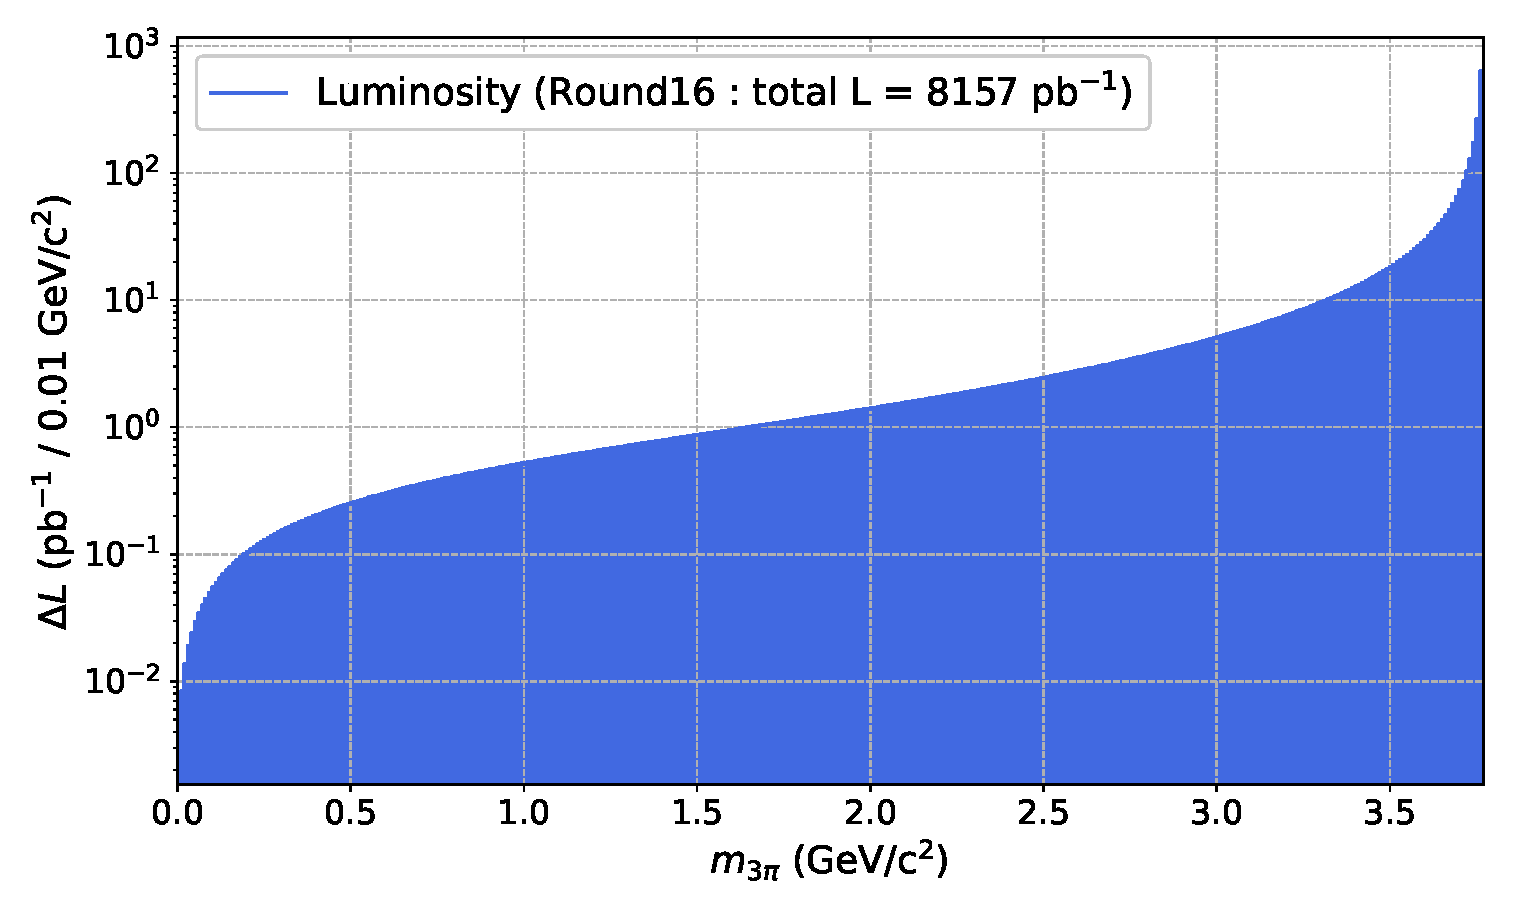
\includegraphics[width=0.45\textwidth]{fig/luminosity_spectrum.eps}
    \caption{Effective luminosity spectrum as a function of the $\pi^{+}\pi^{-}\pi^{0}$ invariant mass ($m_{3\pi}$) calculated for round16 with total integrated luminosity $\mathcal{L}_{\text{int}} = 8157~\text{pb}^{-1}$. The spectrum is shown with logarithmic scale on the vertical axis.}
    \label{fig:luminosity_spectrum}
\end{figure}

Based on this method, rough yield estimates for the two processes with
additional $\pi^{0}$, $e^{+}e^{-} \to \pi^{+}\pi^{-}\pi^{0}\pi^{0}$ (non-ISR)
and $e^{+}e^{-} \to \pi^{+}\pi^{-}\pi^{0}\pi^{0}\gamma_{\text{ISR}}$ (ISR),
were calculated for the four data-taking periods (round03/04, round15, round16,
round17). The results are summarized in
Table~\ref{tab:background_yield_estimate}. For the ISR channel, the estimation
relies on the $e^{+}e^{-} \to \pi^{+}\pi^{-}\pi^{0}\pi^{0}$ cross section
measured by the BaBar collaboration~\cite{BaBar2017_4pi0}.

It is important to note that the values listed in the table are initial yield
estimates without any selection efficiency corrections; the actual background
contribution to the signal region is obtained by multiplying these yields by
the corresponding selection efficiency relevant to the specific analysis cuts.
These estimates serve only to confirm that these processes constitute the main
sources of background and to provide guidance for optimizing subsequent
selection criteria.

\begin{table}[t]
    \begin{center}
        \caption{Rough estimates of the expected yields for the two processes with additional $\pi^{0}$ before applying any selection efficiency. The integrated luminosities are taken from Table~\ref{tab:datalumi}. The cross section for $e^{+}e^{-} \to \pi^{+}\pi^{-}\pi^{0}\pi^{0}$ is taken as $\sigma = 0.22$~nb at $\sqrt{s}=3.773$~GeV, while the energy-dependent cross section for the ISR process is derived from the measured $e^{+}e^{-} \to \pi^{+}\pi^{-}\pi^{0}\pi^{0}$ cross section~\cite{BaBar2017_4pi0}. The final background contribution is obtained by multiplying these yields by the corresponding selection efficiency.}
        \vspace{4mm}
        \begin{tabular}{c | c | c}
            \hline \hline
            Data sample (Run period) & $N(e^{+}e^{-} \to \pi^{+}\pi^{-}\pi^{0}\pi^{0})$ & $N(e^{+}e^{-} \to \pi^{+}\pi^{-}\pi^{0}\pi^{0}\gamma_{\text{ISR}})$ \\
            \hline
            round03-04               & 511940                                           & 1142096                                                             \\
            \hline
            round15                  & 872209                                           & 1945825                                                             \\
            \hline
            round16                  & 1424346                                          & 3177597                                                             \\
            \hline
            round17                  & 731817                                           & 1632623                                                             \\
            \hline \hline
        \end{tabular}
        \label{tab:background_yield_estimate}
    \end{center}
\end{table}

The final background yield is then obtained by multiplying the effective
luminosity spectrum by the cross section and a selection-efficiency factor that
varies dynamically with the analysis cuts. This method is used solely to
confirm that $e^{+}e^{-} \to \pi^{+}\pi^{-}\pi^{0}\pi^{0}$ and $e^{+}e^{-} \to
    \pi^{+}\pi^{-}\pi^{0}\pi^{0}\gamma_{\text{ISR}}$ are the dominant backgrounds
and to optimize the selection criteria. It is not used to derive the final
background estimates; precise yields for these two components will be
determined using data-driven methods.
Based on the rough background estimate from $\mathcal{L} \times
\sigma_{\text{hadron}}$, the signal yield was approximated by subtracting the
background from the data, allowing for a preliminary significance calculation.
Using this approach, a figure of merit (FOM) defined as $S / \sqrt{S + B}$ was
constructed to evaluate the signal significance. To optimize the event
selection, a scan over the kinematic fit $\chi^2$ was performed, with the
result for Round~16 shown in Fig.~\ref{fig:chisq_optimization_round16}.  
The Round~16 optimization yields an optimal cut of $\chi^{2}_{\mathrm{KF}} < 50$. 
As shown in Fig.~\ref{fig:chisq_optimization_rounds}, consistent convergence of 
significance is also observed for Rounds~03/04, 15, and 17 with the same cut.

\begin{figure}[htbp]
    \centering
    \subfloat[$\chi^2$ distribution for the 4C kinematic fit]{
        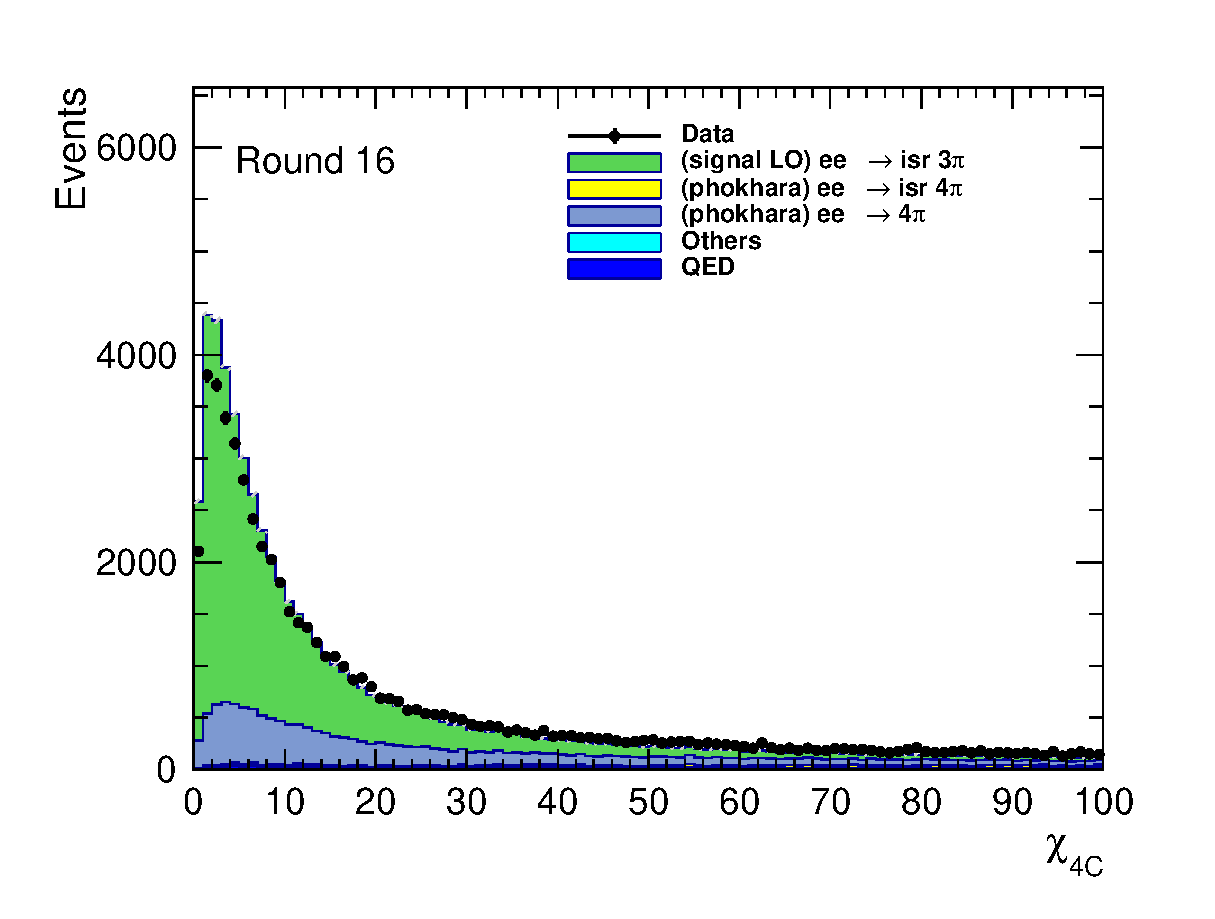
\includegraphics[width=0.48\textwidth]{fig/kmfitchisq_round16.eps}
        \label{fig:kmfitchisq_round16}
    }
    \hfill
    \subfloat[FOM scan as a function of the $\chi^2$ cut]{
        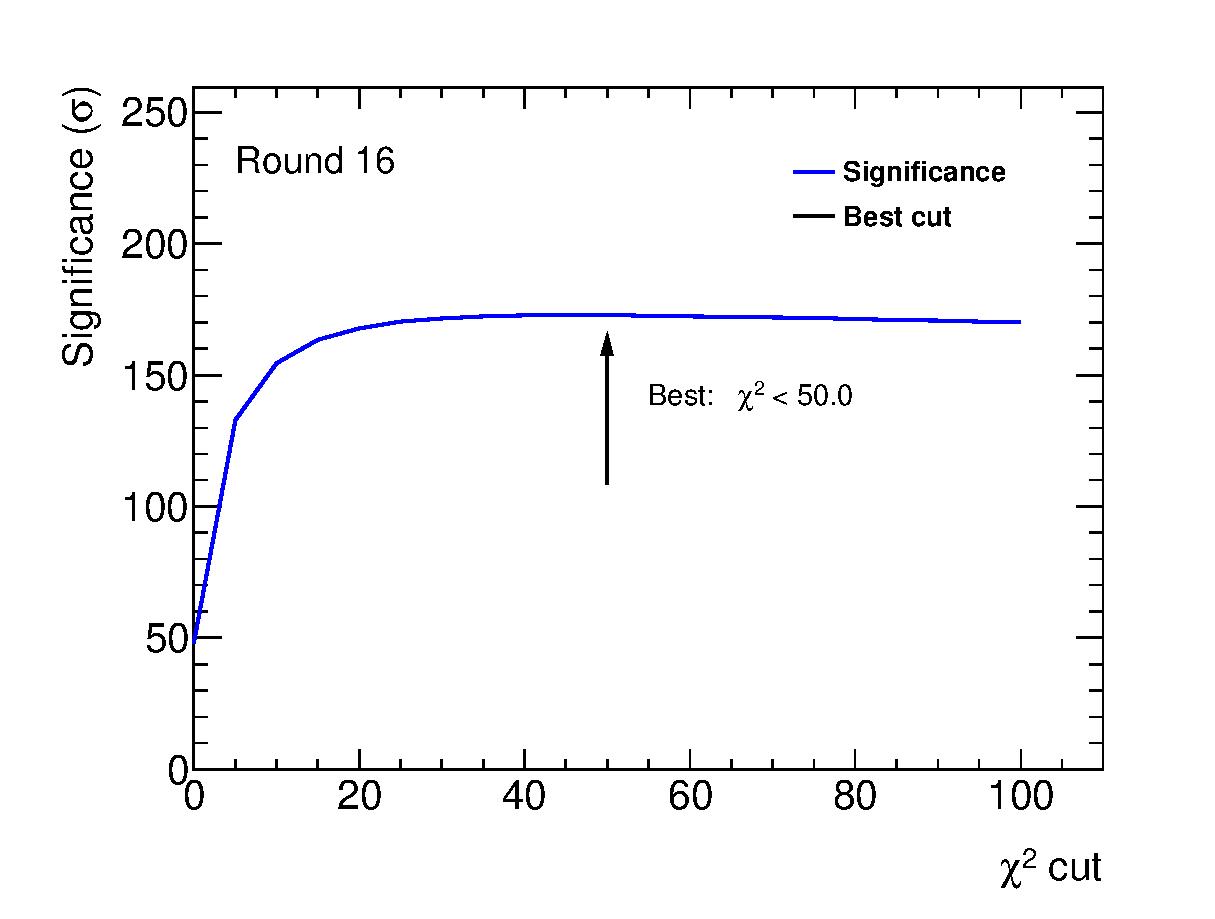
\includegraphics[width=0.48\textwidth]{fig/OptimizeChisq4C_scan_round16.eps}
        \label{fig:optimize_chisq_scan_round16}
    }
    \caption{(a) Distribution of the kinematic fit $\chi^2$ for the four-constraint (4C) fit using the Round~16 data sample. (b) The corresponding figure of merit ($S/\sqrt{S+B}$) as a function of the applied $\chi^2$ cut value for the Round~16 data.}
    \label{fig:chisq_optimization_round16}
\end{figure}

\begin{figure}[htbp]
    \centering
    \subfloat[Round 03/04]{
        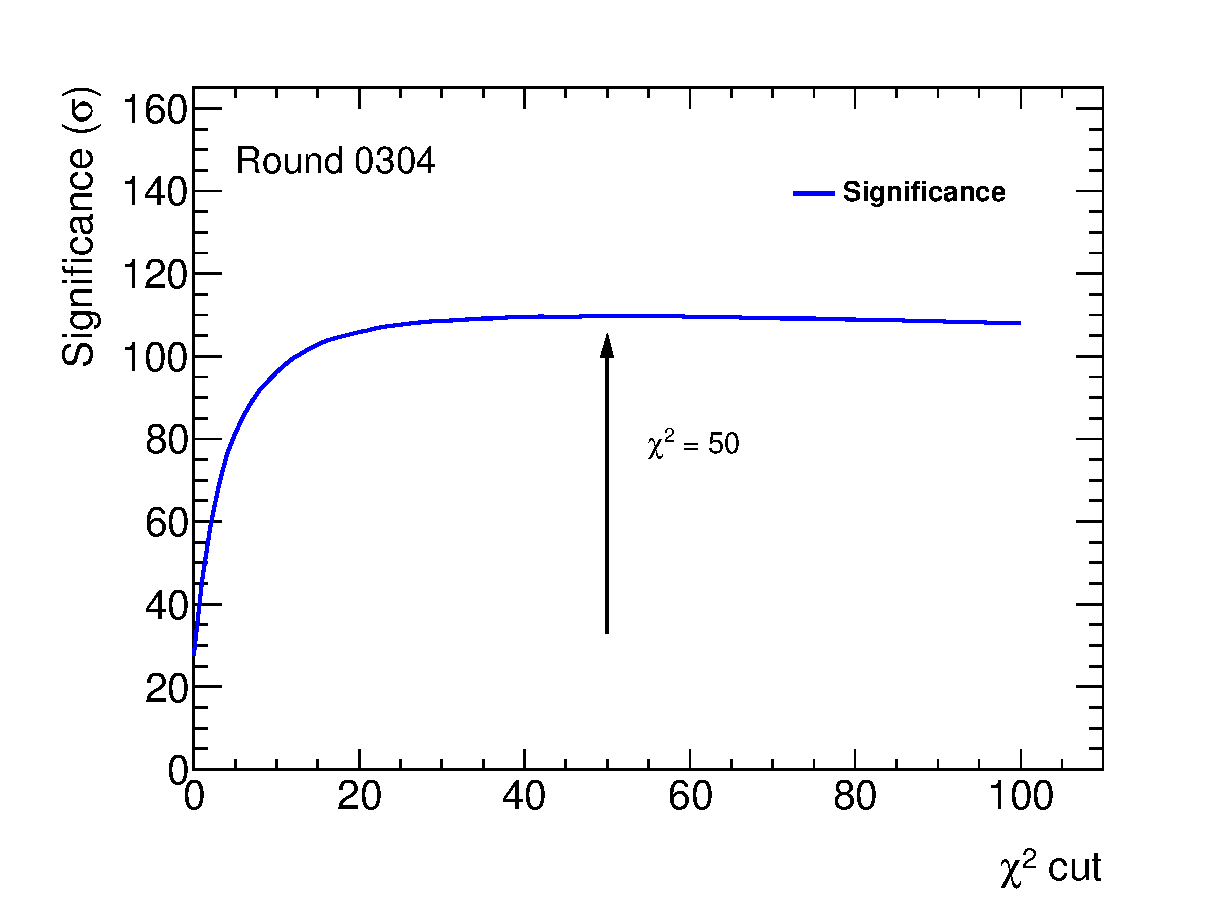
\includegraphics[width=0.40\textwidth]{fig/OptimizeChisq4C_scan_round0304.eps}
        \label{fig:optimize_chisq_scan_round0304}
    }
    \hfill
    \subfloat[Round 15]{
        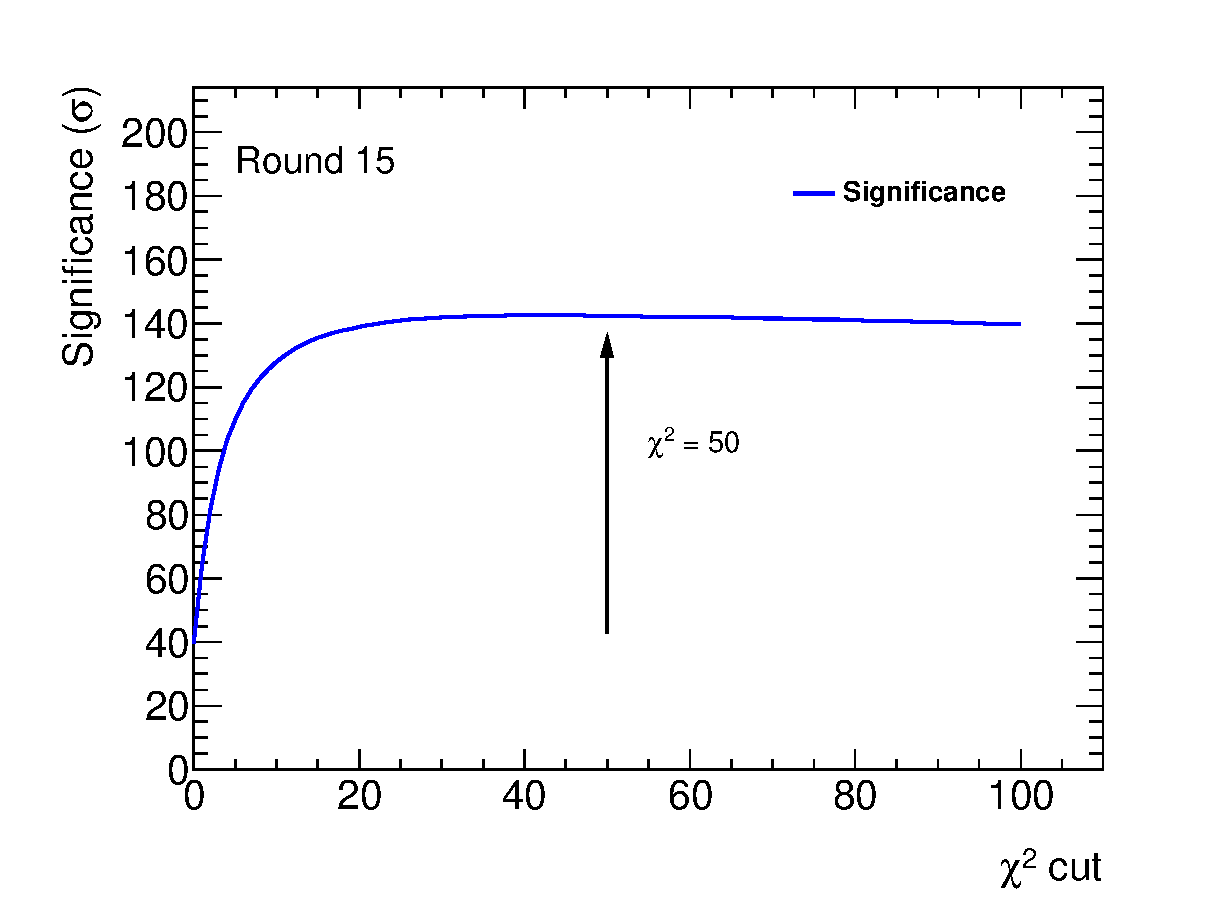
\includegraphics[width=0.40\textwidth]{fig/OptimizeChisq4C_scan_round15.eps}
        \label{fig:optimize_chisq_scan_round15}
    }
    \hfill
    \subfloat[Round 17]{
        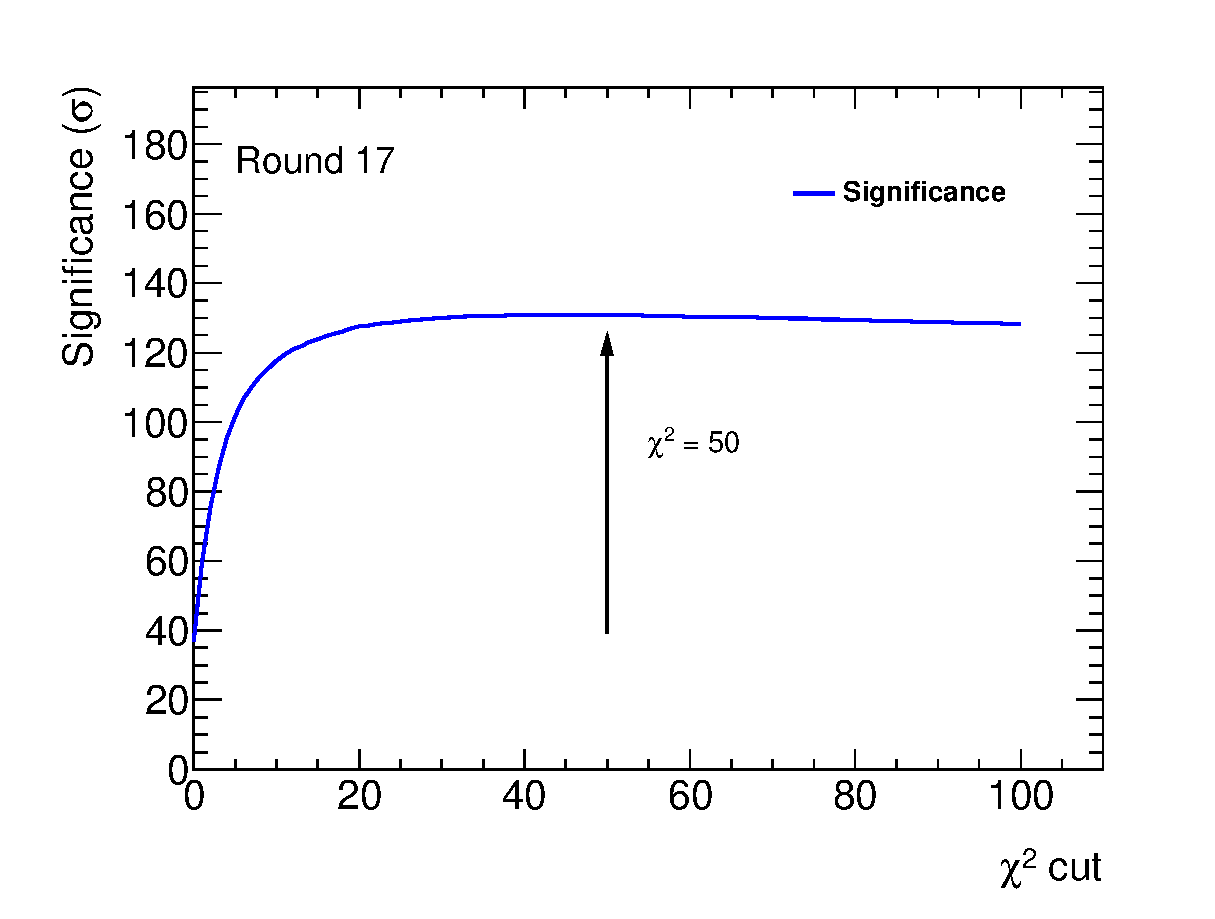
\includegraphics[width=0.40\textwidth]{fig/OptimizeChisq4C_scan_round17.eps}
        \label{fig:optimize_chisq_scan_round17}
    }
    \caption{FOM ($S/\sqrt{S+B}$) as a function of the applied $\chi^2$ cut value for (a) Round~03/04, (b) Round~15, and (c) Round~17 data samples.}
    \label{fig:chisq_optimization_rounds}
\end{figure}

Based on the optimal $\chi^2_{\mathrm{KF}}$ selection, the invariant mass
spectrum of the $3\pi$ system ($M_{3\pi}$) can be divided into three distinct
regions for further study: the $\omega(782)$ region, the $\phi(1020)$ region,
and a higher-mass region associated with possible
$\omega^{\prime}/\omega^{\prime\prime}$ excitations. In the high-mass
$\omega^{\prime}/\omega^{\prime\prime}$ region, a significant background
component from events containing additional $\pi^0$ mesons was observed. To
quantify this, the number of $\pi^0$ candidates per event was counted, where
any $\pi^0$ candidate satisfying a one-constraint kinematic fit $\chi^2 < 200$
was accepted. The distribution of this $\pi^0$ multiplicity is shown in
Fig.~\ref{fig:pi0_multiplicity}. To suppress this specific background, a
requirement of exactly one $\pi^0$ candidate per event was applied exclusively
in the $\omega^{\prime}/\omega^{\prime\prime}$ mass region. No such restriction
was applied to the $\omega(782)$ and $\phi(1020)$ signal regions. The following
studies and distributions are based on the Round~16 data sample.

\begin{figure}[htbp]
    \centering
    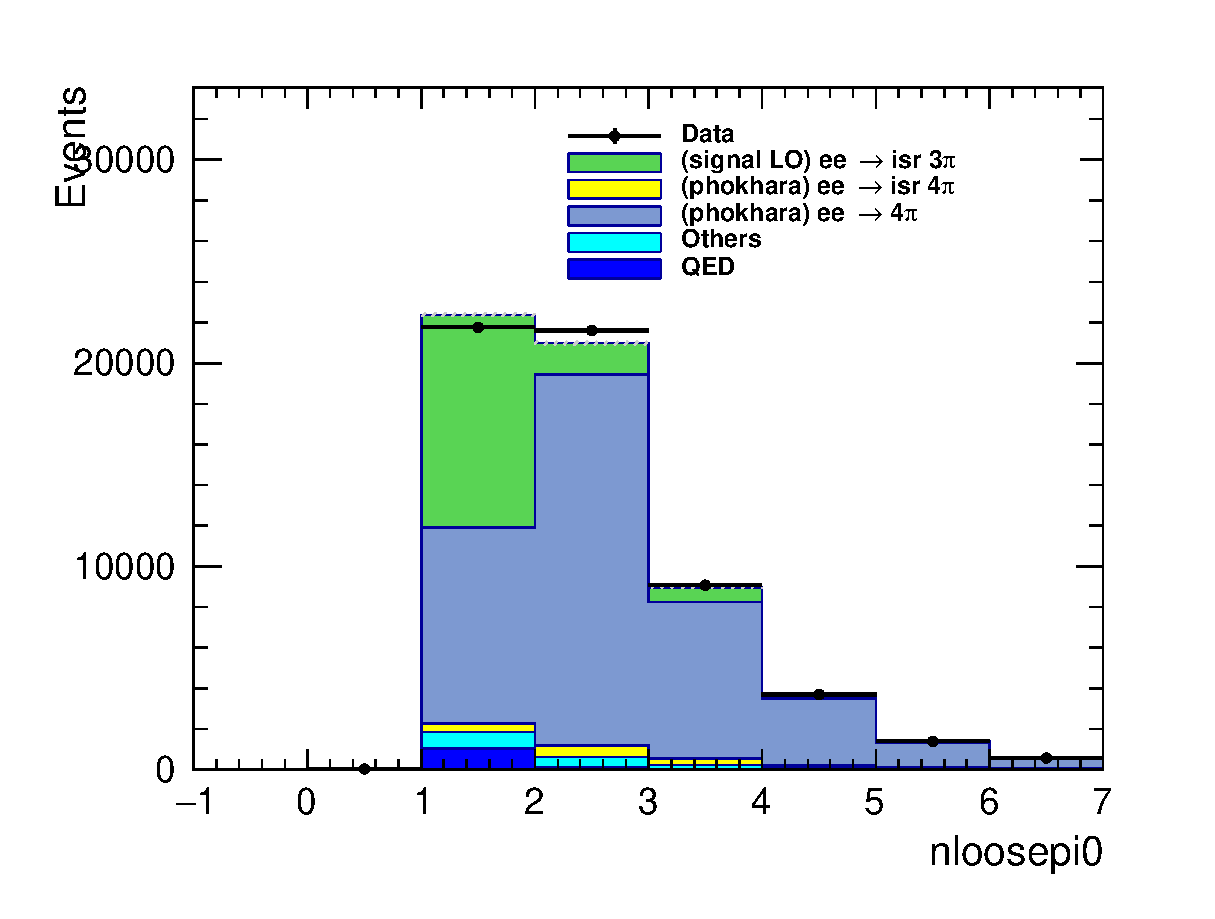
\includegraphics[width=0.45\textwidth]{fig/nloosepi0_origin.eps}
    \caption{Distribution of the number of $\pi^0$ candidates per event in the $\omega^{\prime}/\omega^{\prime\prime}$ mass region using the Round~16 data. A $\pi^0$ candidate is counted if its 1C kinematic fit $\chi^2 < 200$.}
    \label{fig:pi0_multiplicity}
\end{figure}

The resulting $M_{3\pi}$ invariant mass spectra, after applying all selection
criteria including the region-specific $\pi^0$ multiplicity cut, are presented
separately for the three mass regions in
Fig.~\ref{fig:all_rounds_3pi}. The $e^{+}e^{-} \to
    \pi^{+}\pi^{-}\pi^{0}\pi^{0}\gamma_{\text{ISR}}$ contribution is negligible and
will not be treated as a separate background in the subsequent fitting
procedure; only the non-ISR $e^{+}e^{-} \to \pi^{+}\pi^{-}\pi^{0}\pi^{0}$
process will be explicitly estimated using data-driven methods and constrained
in the fit.
\begin{figure}[htbp]
\centering

% === Row 1: Round 03/04 ===
\subfloat[Round 03/04, $\omega(782)$]{
    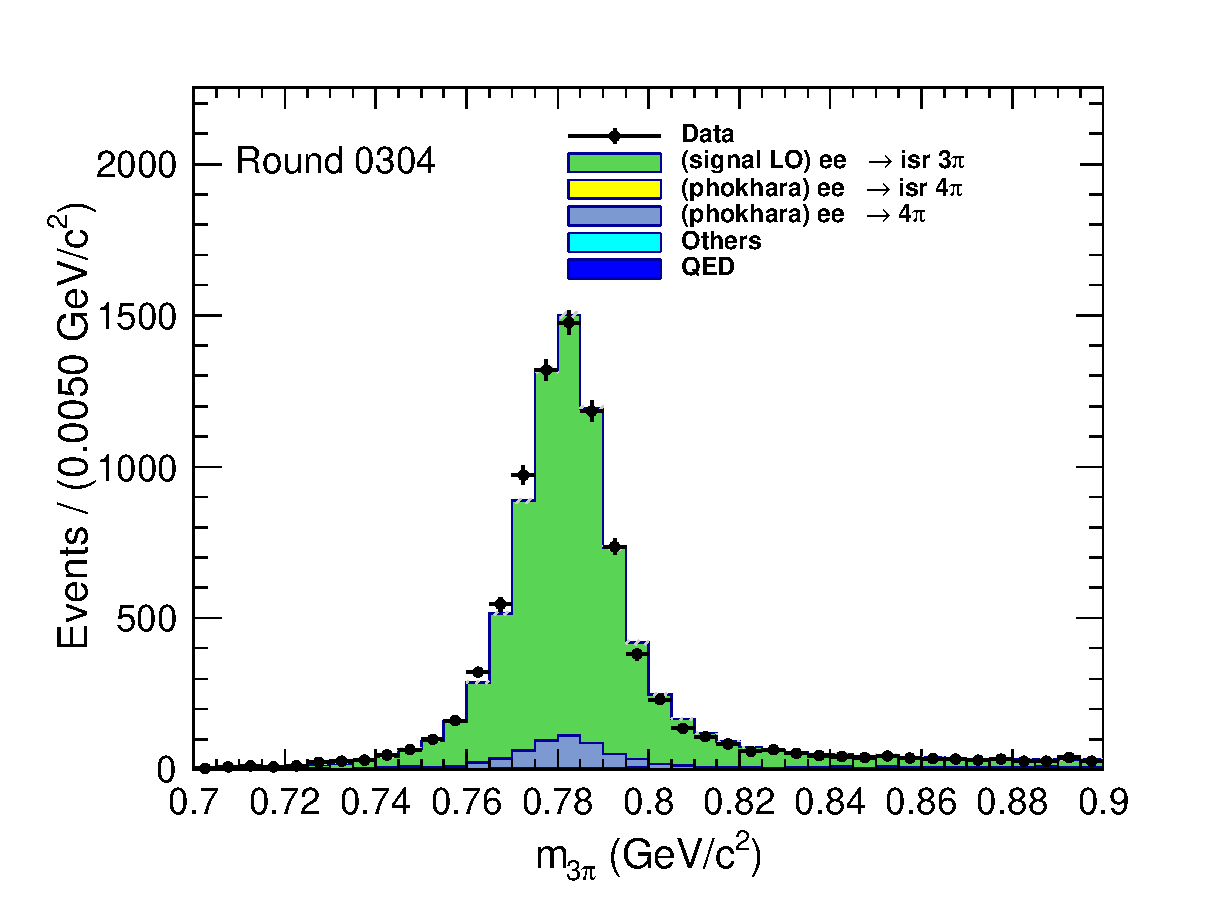
\includegraphics[width=0.32\textwidth]{fig/round0304_omega.eps}
    \label{fig:r0304_omega}
}\hfill
\subfloat[Round 03/04, $\phi(1020)$]{
    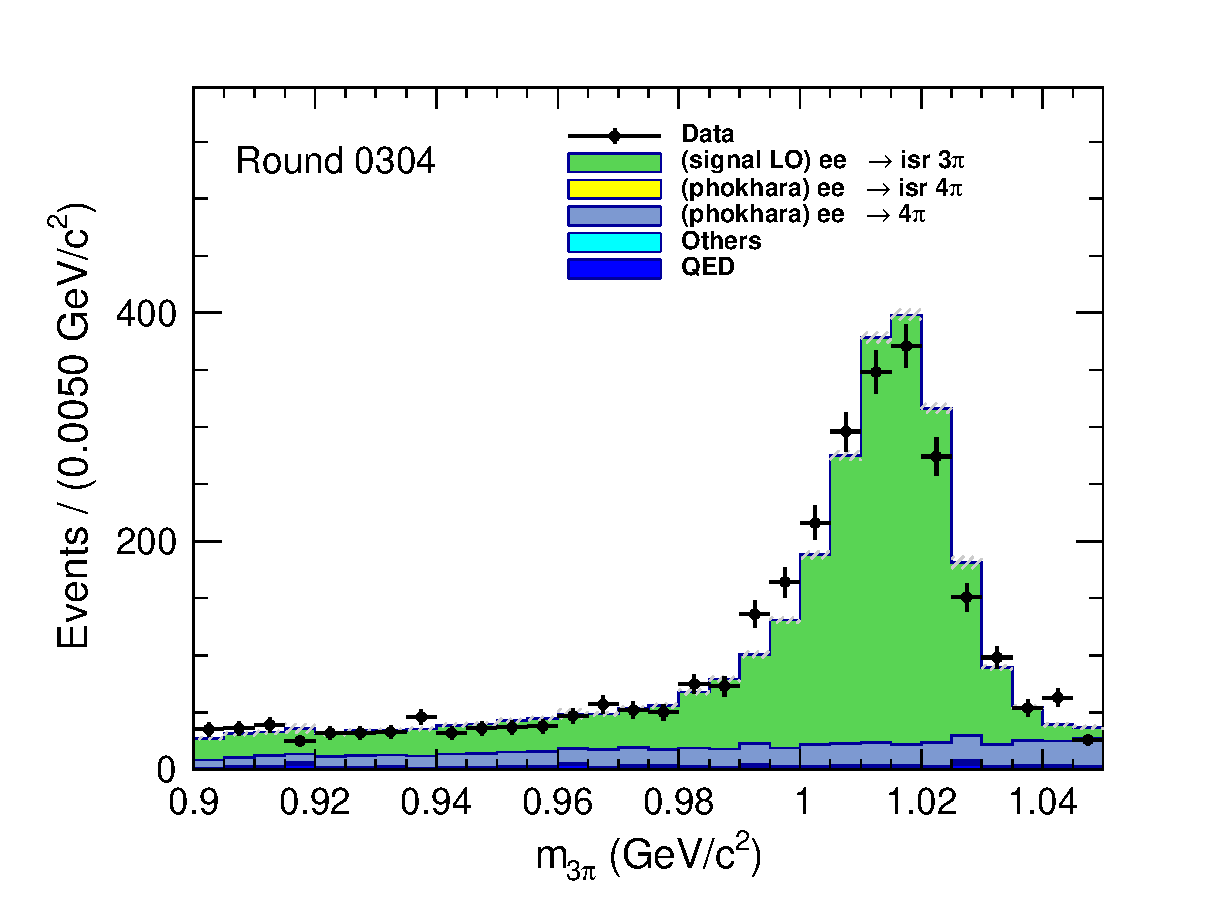
\includegraphics[width=0.32\textwidth]{fig/round0304_phi.eps}
    \label{fig:r0304_phi}
}\hfill
\subfloat[Round 03/04, $\omega^{\prime}/\omega^{\prime\prime}$]{
    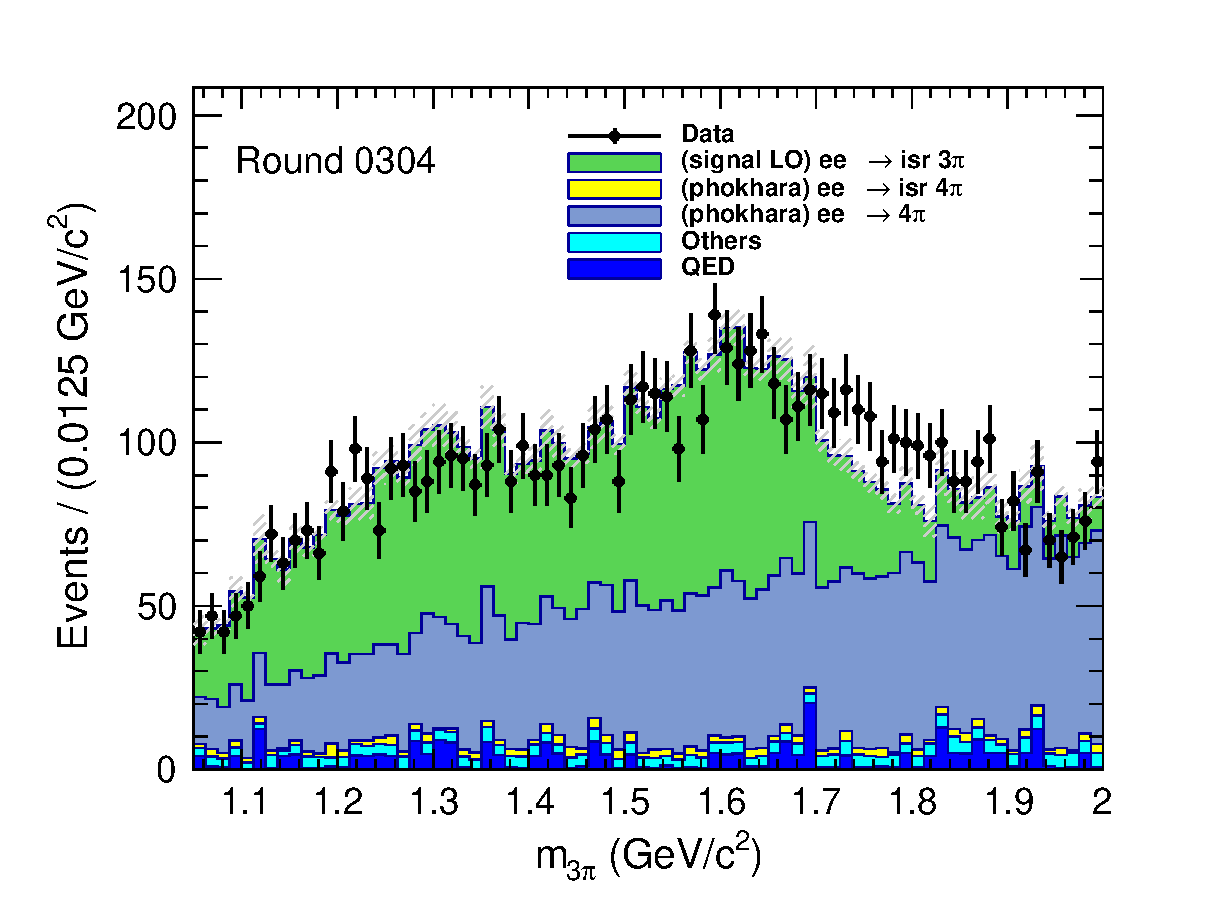
\includegraphics[width=0.32\textwidth]{fig/round0304_omegaprime.eps}
    \label{fig:r0304_omegaprime}
}

% \vspace{0.5\baselineskip}

% === Row 2: Round 15 ===
\subfloat[Round 15, $\omega(782)$]{
    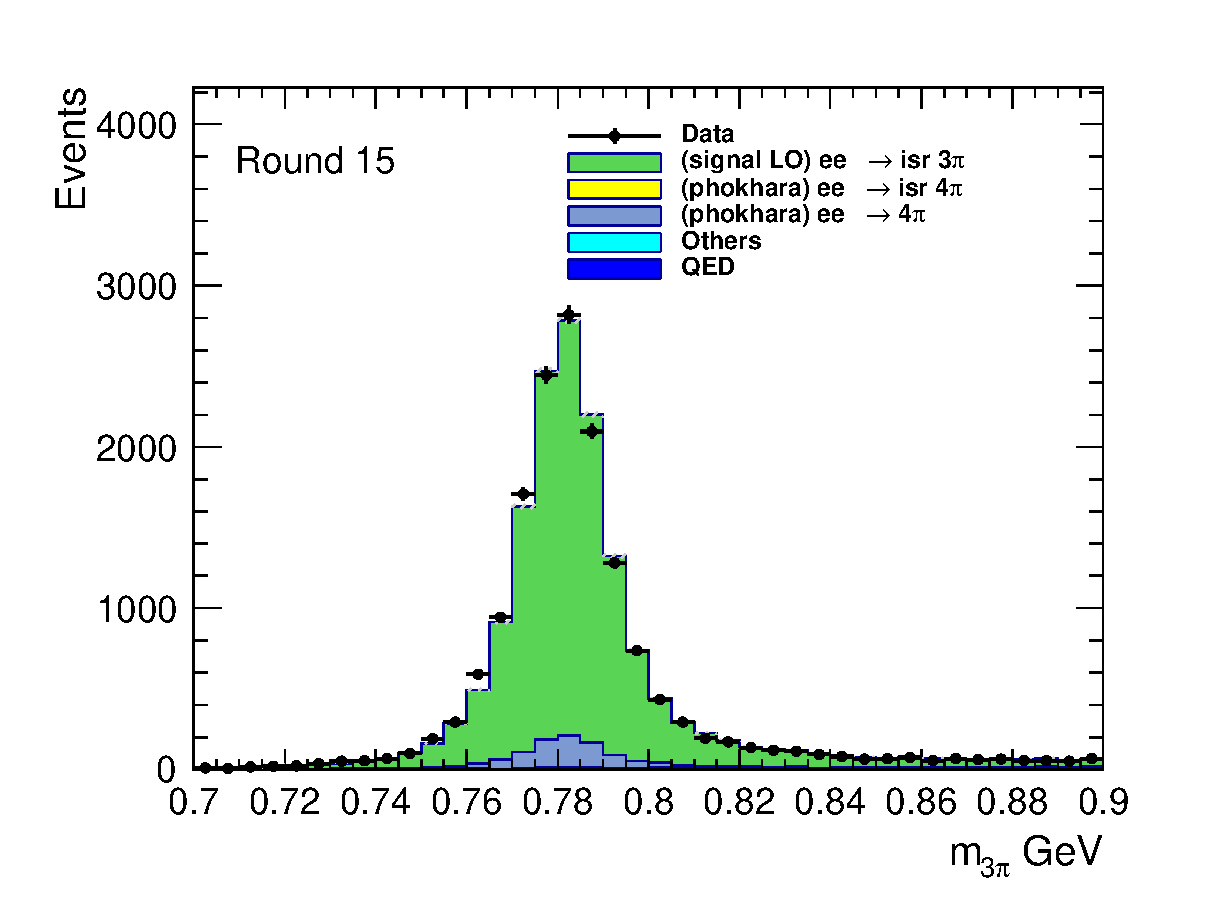
\includegraphics[width=0.32\textwidth]{fig/round15_omega.eps}
    \label{fig:r15_omega}
}\hfill
\subfloat[Round 15, $\phi(1020)$]{
    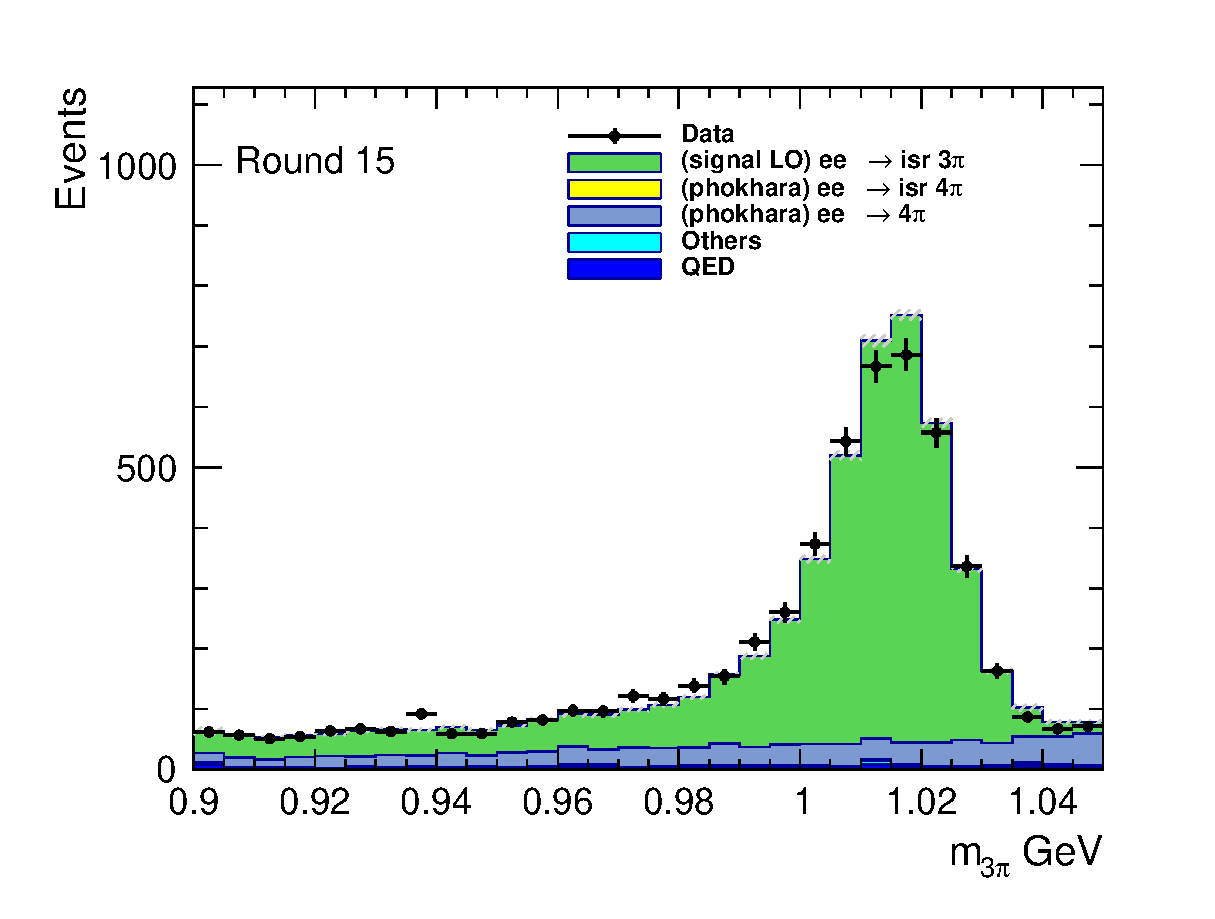
\includegraphics[width=0.32\textwidth]{fig/round15_phi.eps}
    \label{fig:r15_phi}
}\hfill
\subfloat[Round 15, $\omega^{\prime}/\omega^{\prime\prime}$]{
    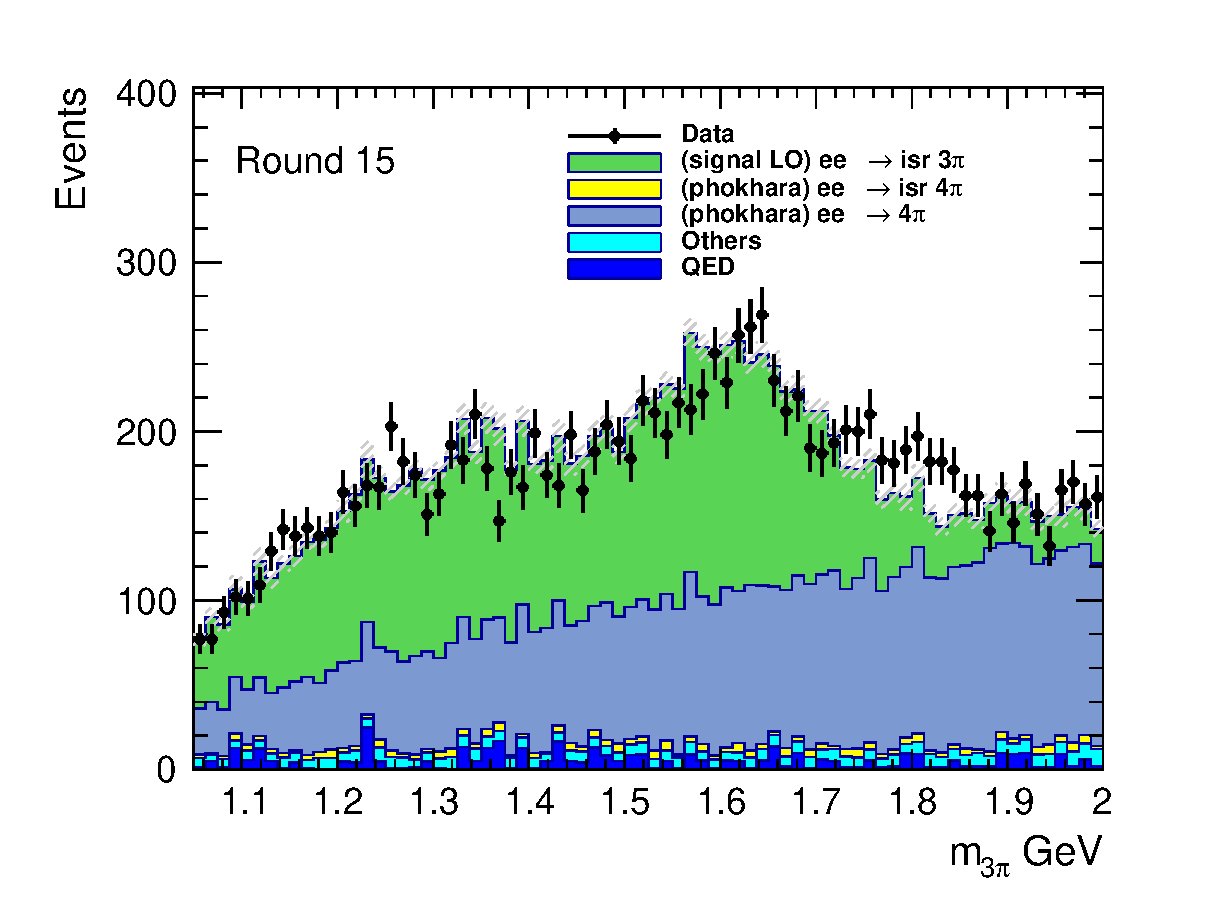
\includegraphics[width=0.32\textwidth]{fig/round15_omegaprime.eps}
    \label{fig:r15_omegaprime}
}

% \vspace{0.5\baselineskip}

% === Row 3: Round 16 ===
\subfloat[Round 16, $\omega(782)$]{
    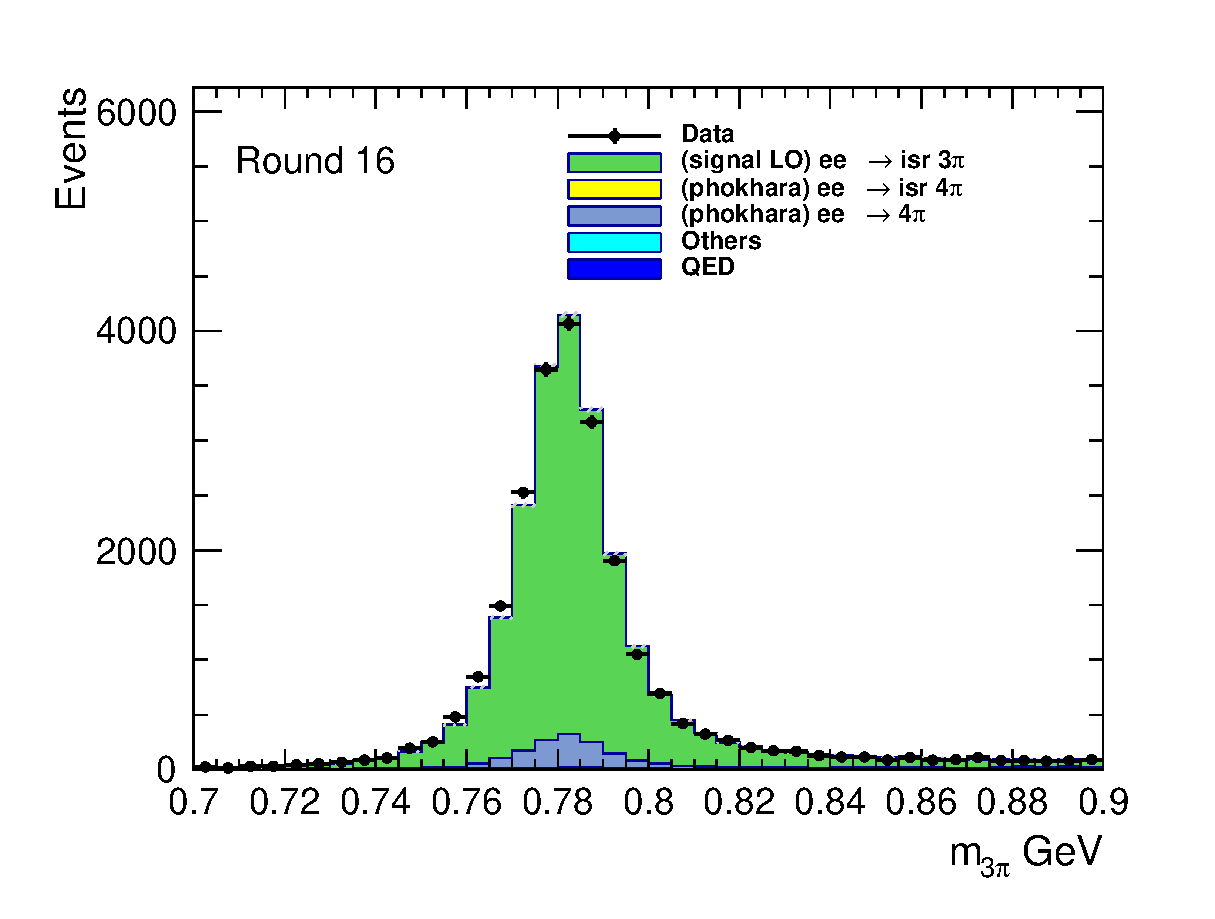
\includegraphics[width=0.32\textwidth]{fig/round16_omega.eps}
    \label{fig:r16_omega}
}\hfill
\subfloat[Round 16, $\phi(1020)$]{
    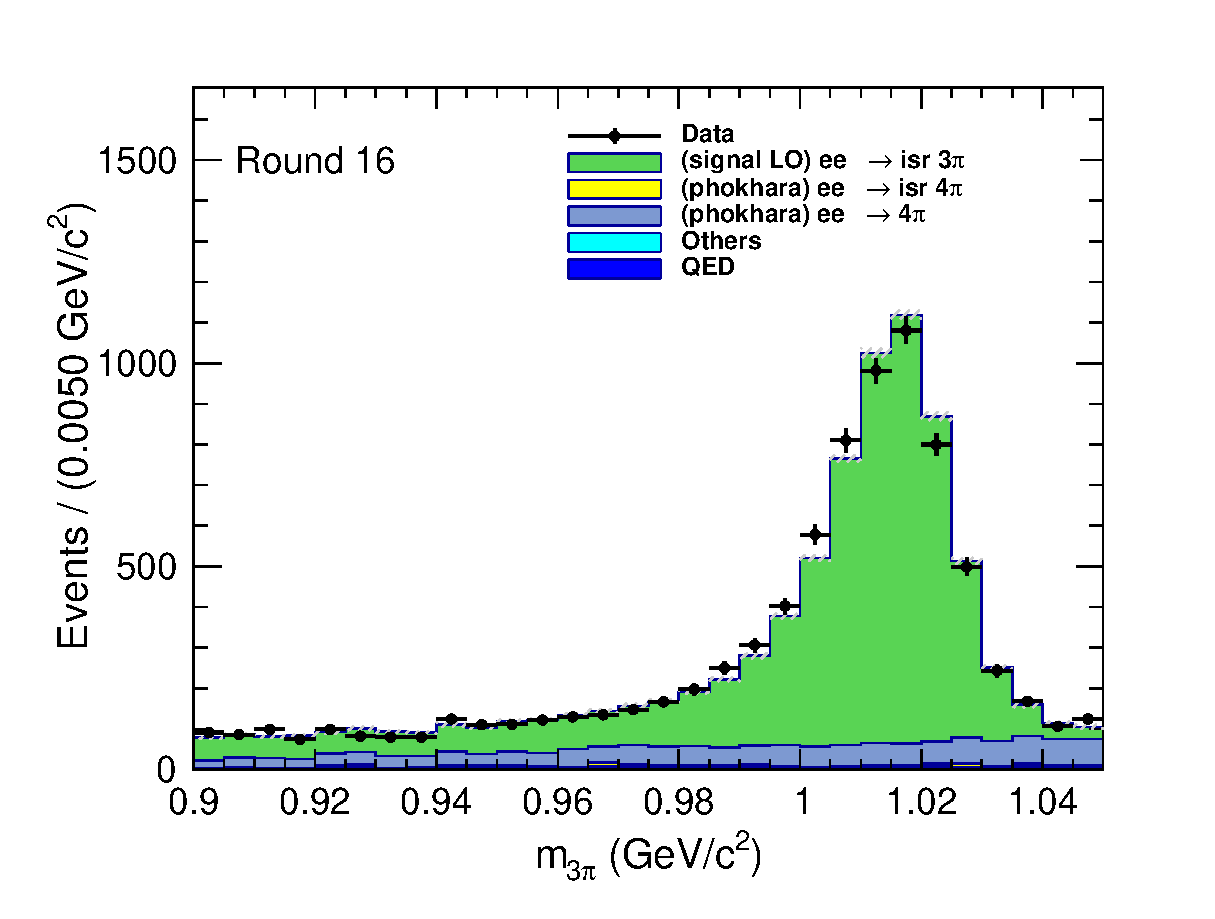
\includegraphics[width=0.32\textwidth]{fig/round16_phi.eps}
    \label{fig:r16_phi}
}\hfill
\subfloat[Round 16, $\omega^{\prime}/\omega^{\prime\prime}$]{
    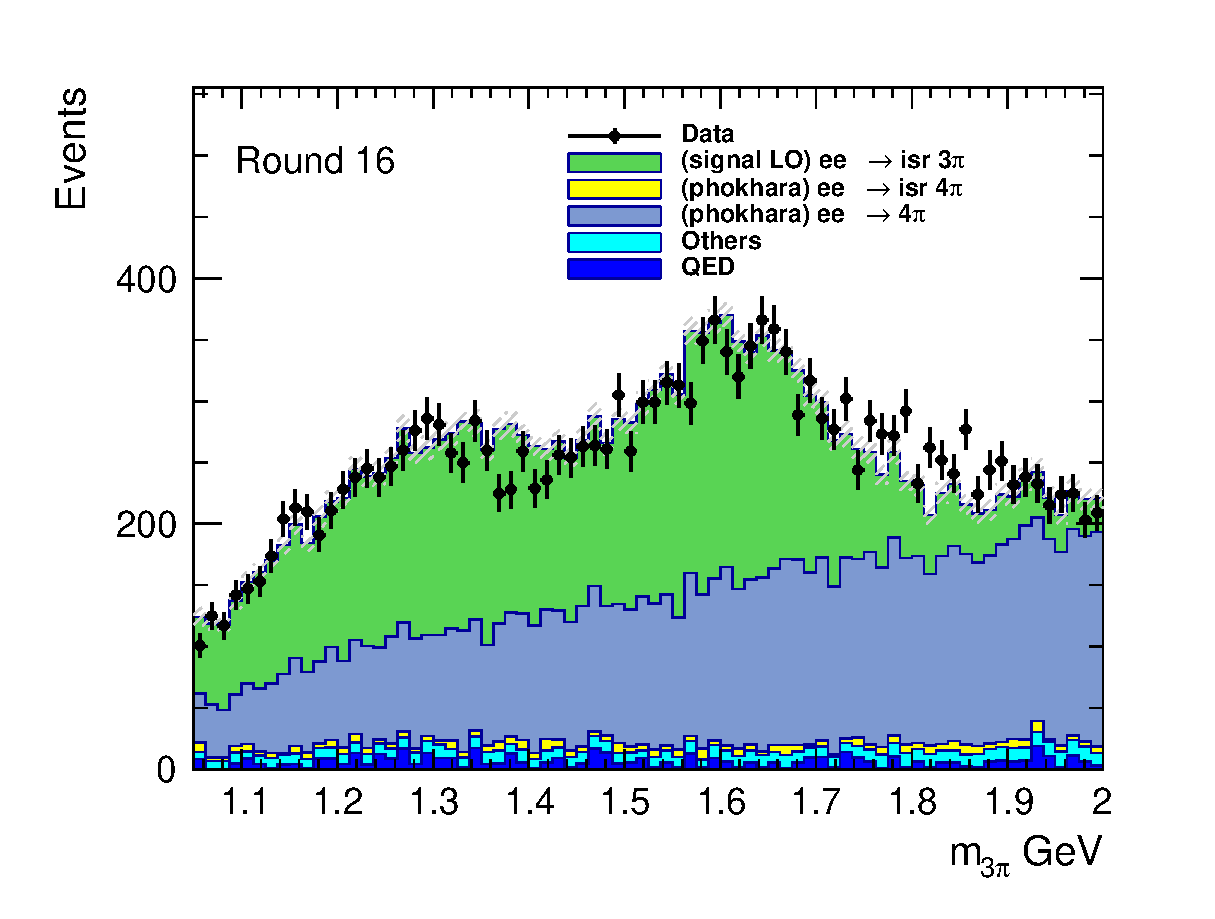
\includegraphics[width=0.32\textwidth]{fig/round16_omegaprime.eps}
    \label{fig:r16_omegaprime}
}

% \vspace{0.5\baselineskip}

% === Row 4: Round 17 ===
\subfloat[Round 17, $\omega(782)$]{
    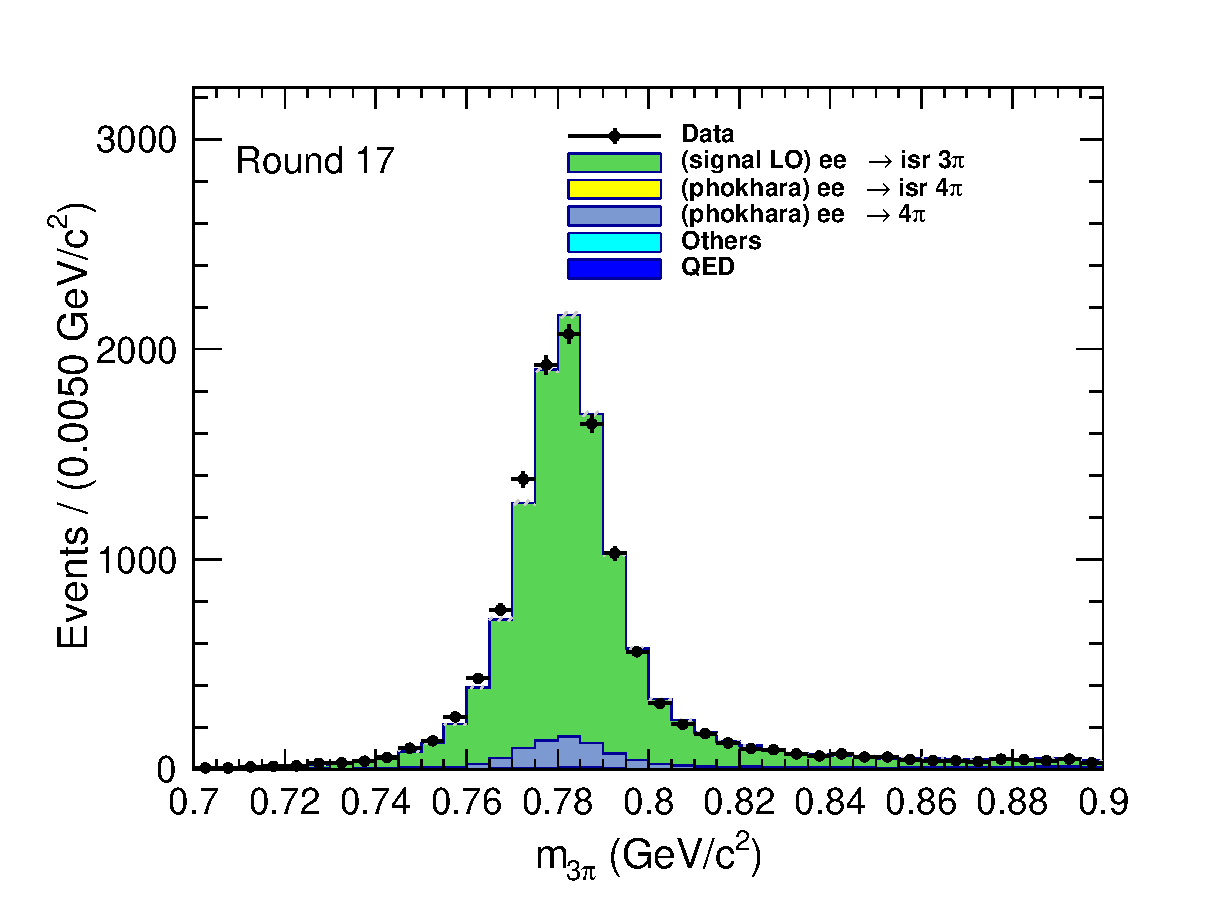
\includegraphics[width=0.32\textwidth]{fig/round17_omega.eps}
    \label{fig:r17_omega}
}\hfill
\subfloat[Round 17, $\phi(1020)$]{
    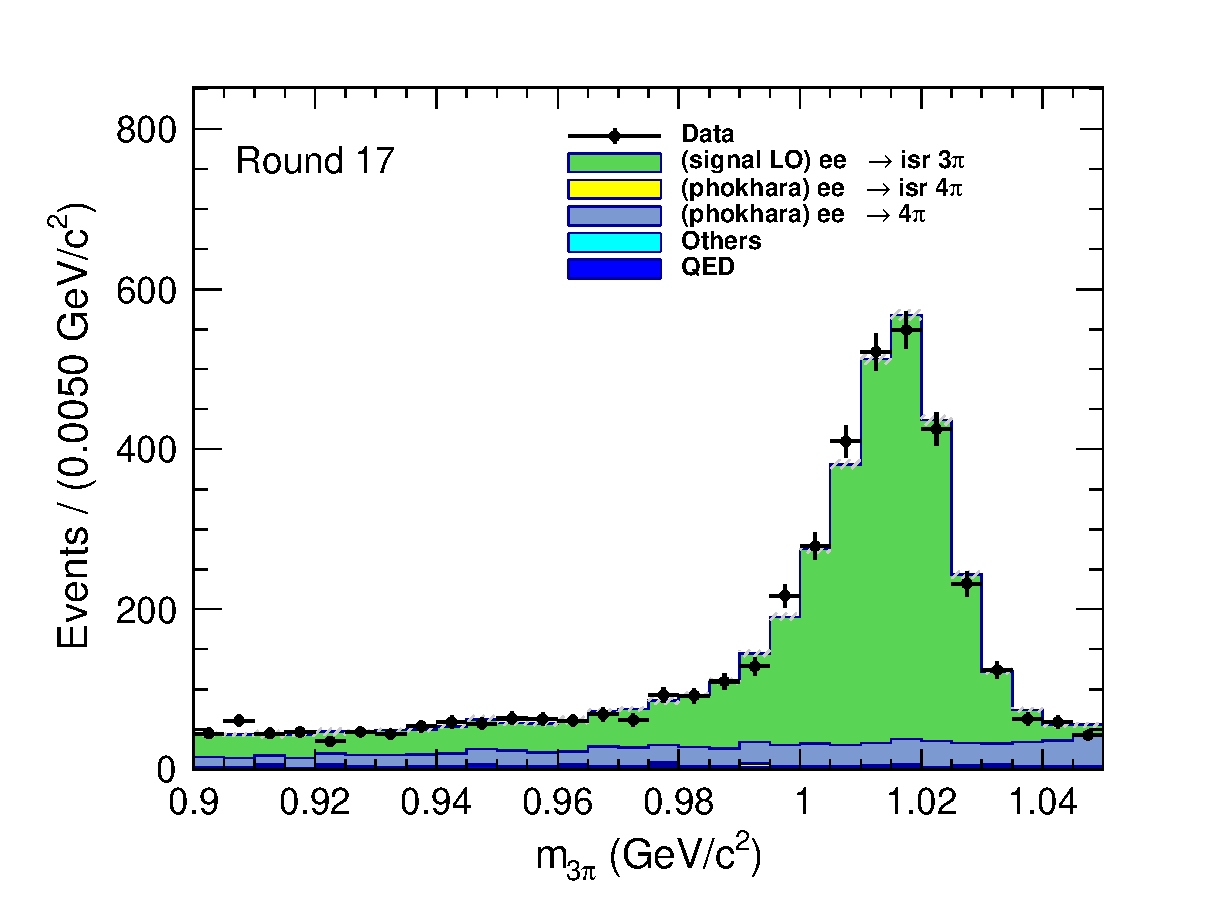
\includegraphics[width=0.32\textwidth]{fig/round17_phi.eps}
    \label{fig:r17_phi}
}\hfill
\subfloat[Round 17, $\omega^{\prime}/\omega^{\prime\prime}$]{
    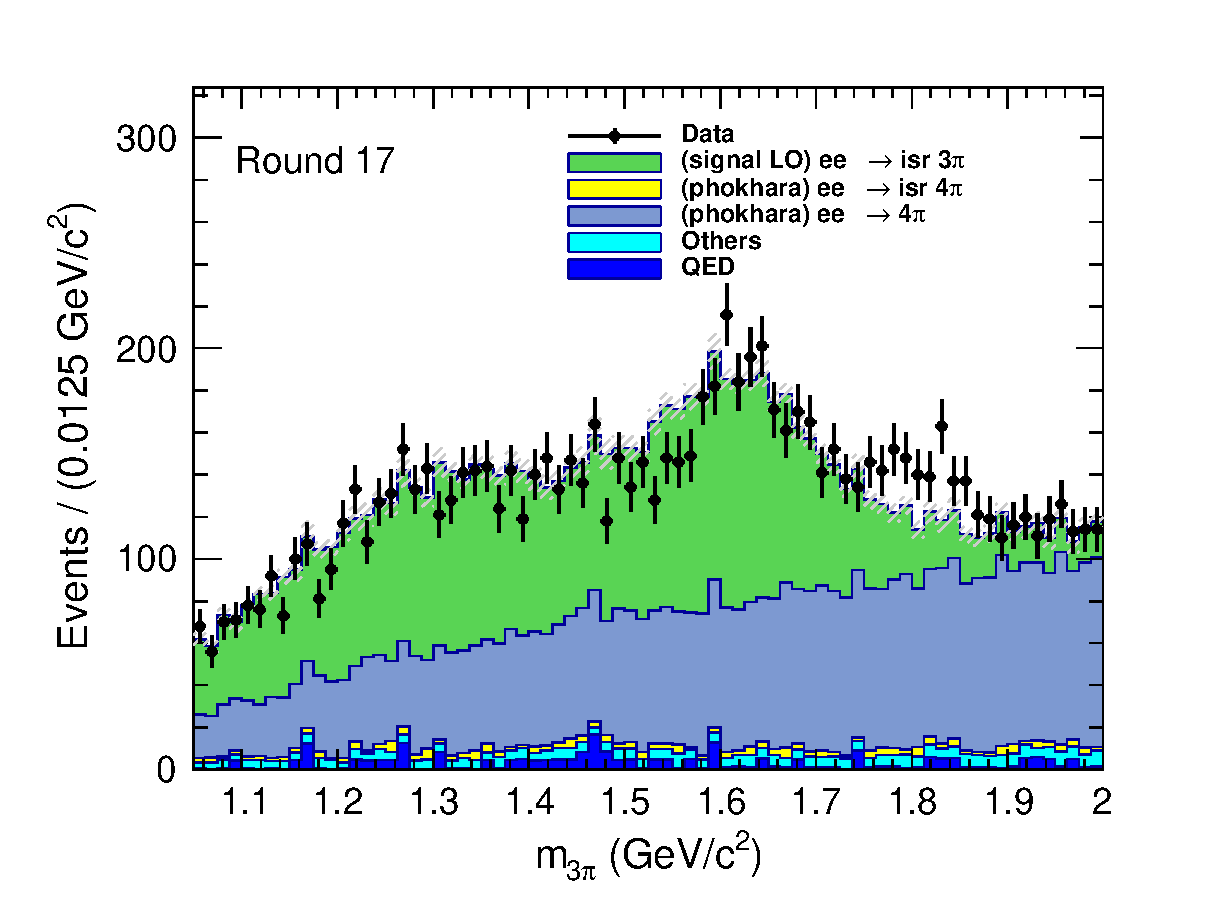
\includegraphics[width=0.32\textwidth]{fig/round17_omegaprime.eps}
    \label{fig:r17_omegaprime}
}

\caption{Invariant mass spectra $M_{3\pi}$ for different data rounds and mass regions with $N_{\pi^0}=1$ (other columns no $\pi^0$ multiplicity cut).}
\label{fig:all_rounds_3pi}
\end{figure}
% The $3\pi$ invariant mass distribution obtained with the $\chi^{2}_{\mathrm{KF}} < 50$ selection is presented in Fig.~\ref{fig:mass3pi_stacked}. This plot, using the Round~16 data sample, displays the data in comparison with the stacked MC predictions for the signal and background components.

% \begin{figure}[htbp]
%     \centering
%     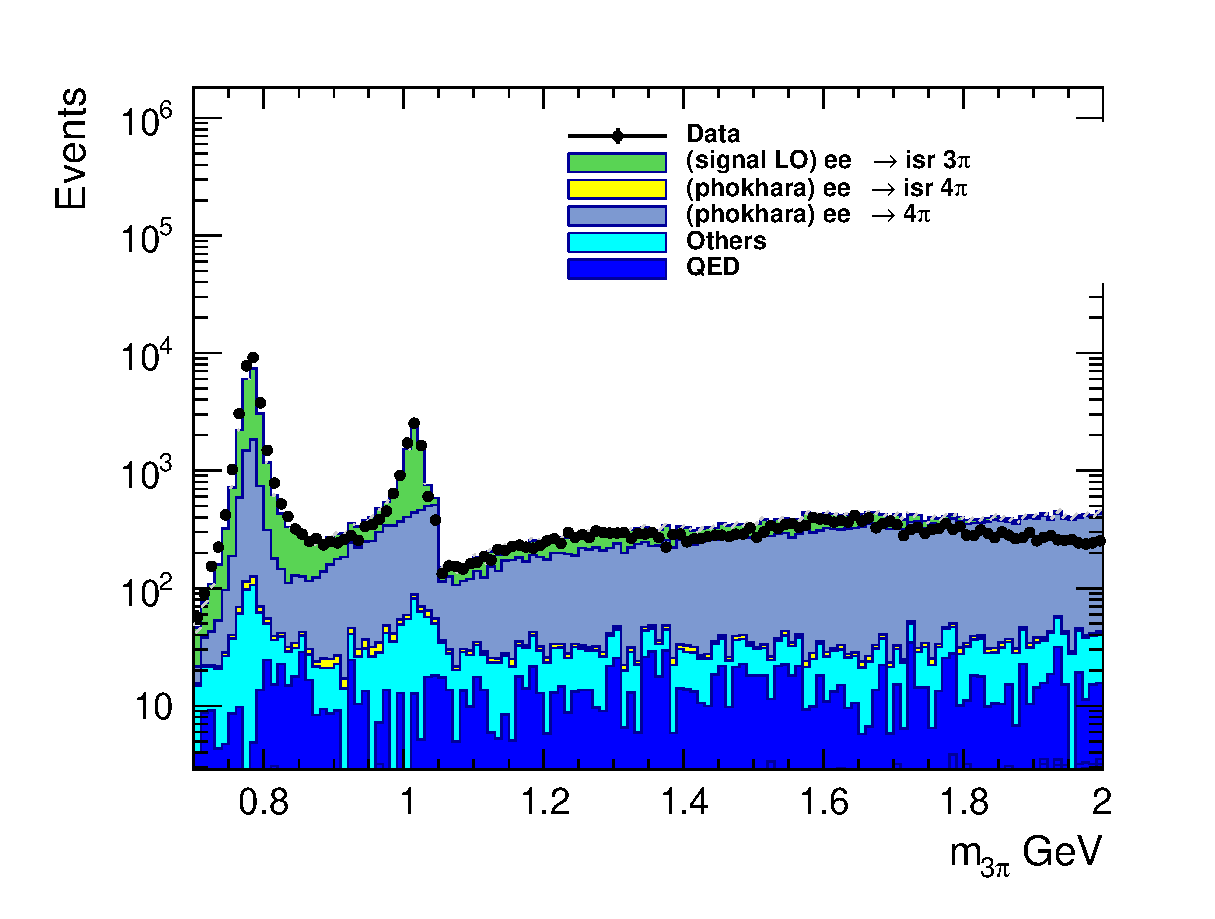
\includegraphics[width=0.6\textwidth]{fig/mass3pi.eps}
%     \caption{The $3\pi$ invariant mass distribution after applying the $\chi^{2}_{\mathrm{KF}} < 50$ selection to the Round~16 data sample. The stacked histogram shows the contributions from the signal process $e^{+}e^{-} \to \pi^{+}\pi^{-}\pi^{0}$ and various background processes, including the dominant $e^{+}e^{-} \to \pi^{+}\pi^{-}\pi^{0}\pi^{0}$ and $e^{+}e^{-} \to \pi^{+}\pi^{-}\pi^{0}\pi^{0}\gamma_{\text{ISR}}$ backgrounds.}
%     \label{fig:mass3pi_stacked}
% \end{figure}

\clearpage
\subsection{Estimate of $\ee\to\pip\pim\piz\piz$}
In estimating the $e^{+}e^{-} \to \pi^{+}\pi^{-}\pi^{0}\pi^{0}$ background, the
following strategy was adopted:

It is assumed that the total yield of $e^{+}e^{-} \to
    \pi^{+}\pi^{-}\pi^{0}\pi^{0}$ events produced in the data is a fixed quantity.
This process enters our signal region primarily when a photon from one of the
$\pi^{0}$ decays is misidentified as an initial-state radiation photon
($\gamma_{\text{ISR}}$). Consequently, two distinct selection efficiencies can
be calculated: $\epsilon_{\text{sig}}$ (the efficiency for $e^{+}e^{-} \to
    \pi^{+}\pi^{-}\pi^{0}\pi^{0}$ events to be selected as signal candidates) and
$\epsilon_{\text{bkg}}$ (the efficiency for the same process to enter the
$3\pi$ signal region as background).

When $e^{+}e^{-} \to \pi^{+}\pi^{-}\pi^{0}\pi^{0}$ events are selected as
signal, the same analysis procedure as for the signal is applied to construct
the $3\pi$ invariant mass spectrum, thereby obtaining the distribution of this
process in data. Using the ratio of these two efficiencies, $R =
    \epsilon_{\text{bkg}} / \epsilon_{\text{sig}}$, the observed $e^{+}e^{-} \to
    \pi^{+}\pi^{-}\pi^{0}\pi^{0}$ signal distribution can be converted into an
estimate of its background distribution in the signal region. Specifically:
\begin{equation}
    N_{\text{bkg}} = R \times N_{\text{sig}}^{\text{obs}} = \frac{\epsilon_{\text{bkg}}}{\epsilon_{\text{sig}}} \times N_{\text{sig}}^{\text{obs}},
\end{equation}
where $N_{\text{sig}}^{\text{obs}}$ is the number of observed $e^{+}e^{-} \to
    \pi^{+}\pi^{-}\pi^{0}\pi^{0}$ signal events in data, and $N_{\text{bkg}}$ is
the estimated number of background events from this process in the signal
region.

This method provides a data-driven conversion from the observed signal
distribution to the background distribution through efficiency correction.

When treating $e^{+}e^{-} \to \pi^{+}\pi^{-}\pi^{0}\pi^{0}$ as the signal, the
selection criteria are designed such that the same event sample also satisfies
a loose selection for $e^{+}e^{-} \to
    \gamma_{\mathrm{ISR}}\pi^{+}\pi^{-}\pi^{0}$. This ensures that the invariant
mass of the three-pion system is automatically defined within the latter
process.

The combined selection proceeds as follows: events are required to meet the
criteria for both processes. The first step applies the full $e^{+}e^{-} \to
    \pi^{+}\pi^{-}\pi^{0}\pi^{0}$ selection:
\begin{itemize}
    \item \textbf{$\pi^{+}\pi^{-}\pi^{0}\pi^{0}$ Candidate Selection:}
          \begin{itemize}
              \item Exactly two good charged tracks.
              \item $\text{nPi0} \geq 2$ \& \& $\text{nGoodShowers} \geq 4$ (ensuring at least two $\pi^{0}$s).
              \item Application of a total 4-momentum constraint to the initial $e^{+}e^{-}$
                    collision (4C kinematic fit).
              \item The candidate with the minimum $\chi_{\mathrm{4C}}^2$ is chosen.
              \item A requirement of $\chi_{\mathrm{KF}}^{2} < 10$ on the kinematic fit.
          \end{itemize}
\end{itemize}

Subsequently, within the same event, a candidate for $e^{+}e^{-} \to
    \gamma_{\mathrm{ISR}}\pi^{+}\pi^{-}\pi^{0}$ is formed by reinterpreting one of
the $\pi^{0}$s as the $\gamma_{\mathrm{ISR}}$:
\begin{itemize}
    \item \textbf{$\gamma_{\mathrm{ISR}}\pi^{+}\pi^{-}\pi^{0}$ Candidate Selection:}
          \begin{itemize}
              \item The same two good charged tracks.
              \item $\text{nPi0} \geq 1$ \& \& $\text{nGoodShowers} \geq 3$ (ensuring at least one $\pi^{0}$ and one photon assigned as $\gamma_{\mathrm{ISR}}$).
              \item Application of the same total 4-momentum constraint to the initial $e^{+}e^{-}$
                    collision (4C kinematic fit).
              \item The candidate with the minimum $\chi_{\mathrm{4C}}^2$ is chosen.
              \item No additional kinematic fit $\chi^2$ requirement is applied at this stage.
          \end{itemize}
\end{itemize}

This dual-tag strategy guarantees that the reconstructed $3\pi$ system from the
$e^{+}e^{-} \to \gamma_{\mathrm{ISR}}\pi^{+}\pi^{-}\pi^{0}$ hypothesis is
kinematically well-defined, and its invariant mass can be reliably calculated
for the subsequent analysis.

The selection described above results in a highly pure sample of $e^{+}e^{-}
\to \pi^{+}\pi^{-}\pi^{0}\pi^{0}$ events. The invariant mass spectrum of the
corresponding three-pion system from this pure sample, which serves as the
input template for background estimation, is shown in
Fig.~\ref{fig:nonisr4pi_all_rounds_regions}.

\begin{figure}[htbp]
    \centering
    \subfloat[Round 03/04]{
        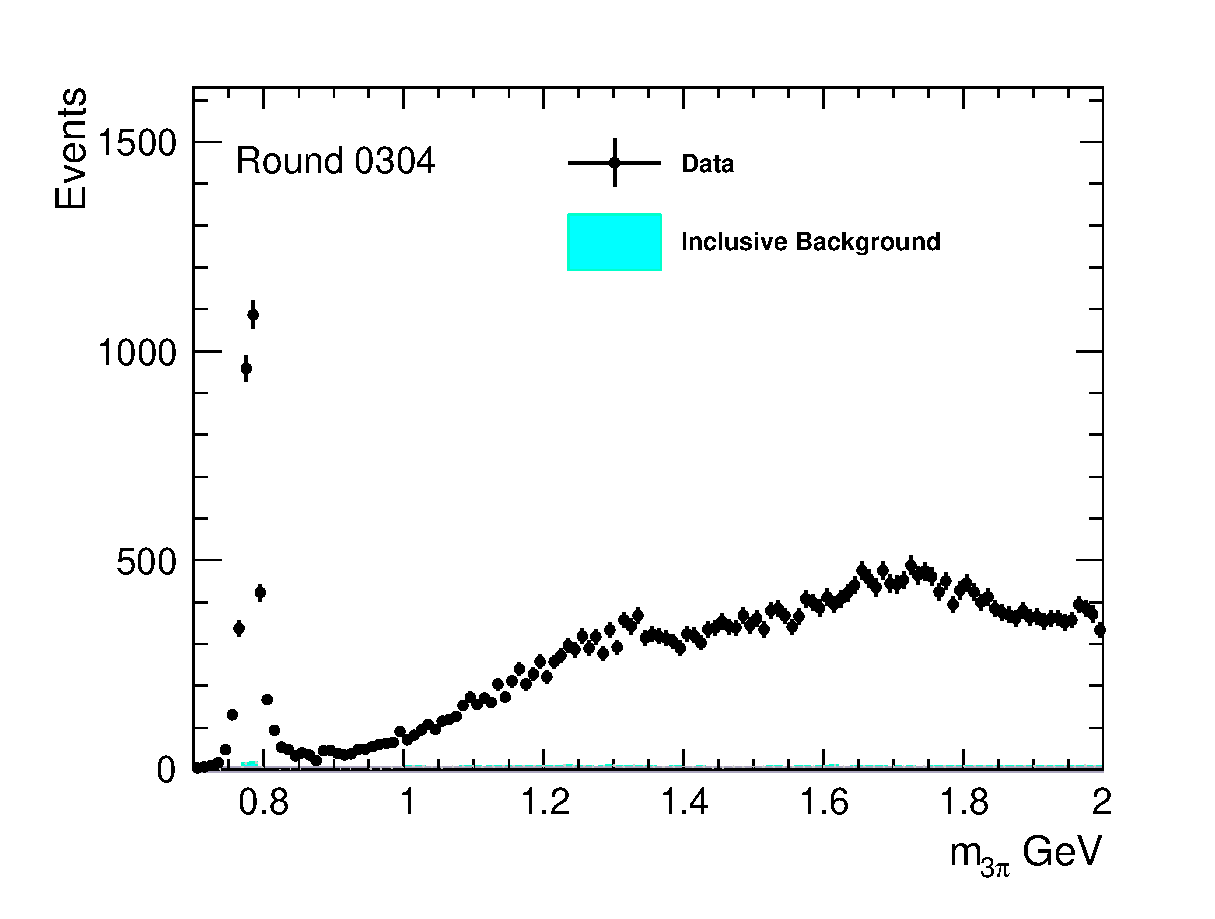
\includegraphics[width=0.40\textwidth]{fig/4pi_3pi_mass_round0304.eps}
        \label{fig:4pi_background_spectrum_round0304}
    }
    \hfill
    \subfloat[Round 15]{
        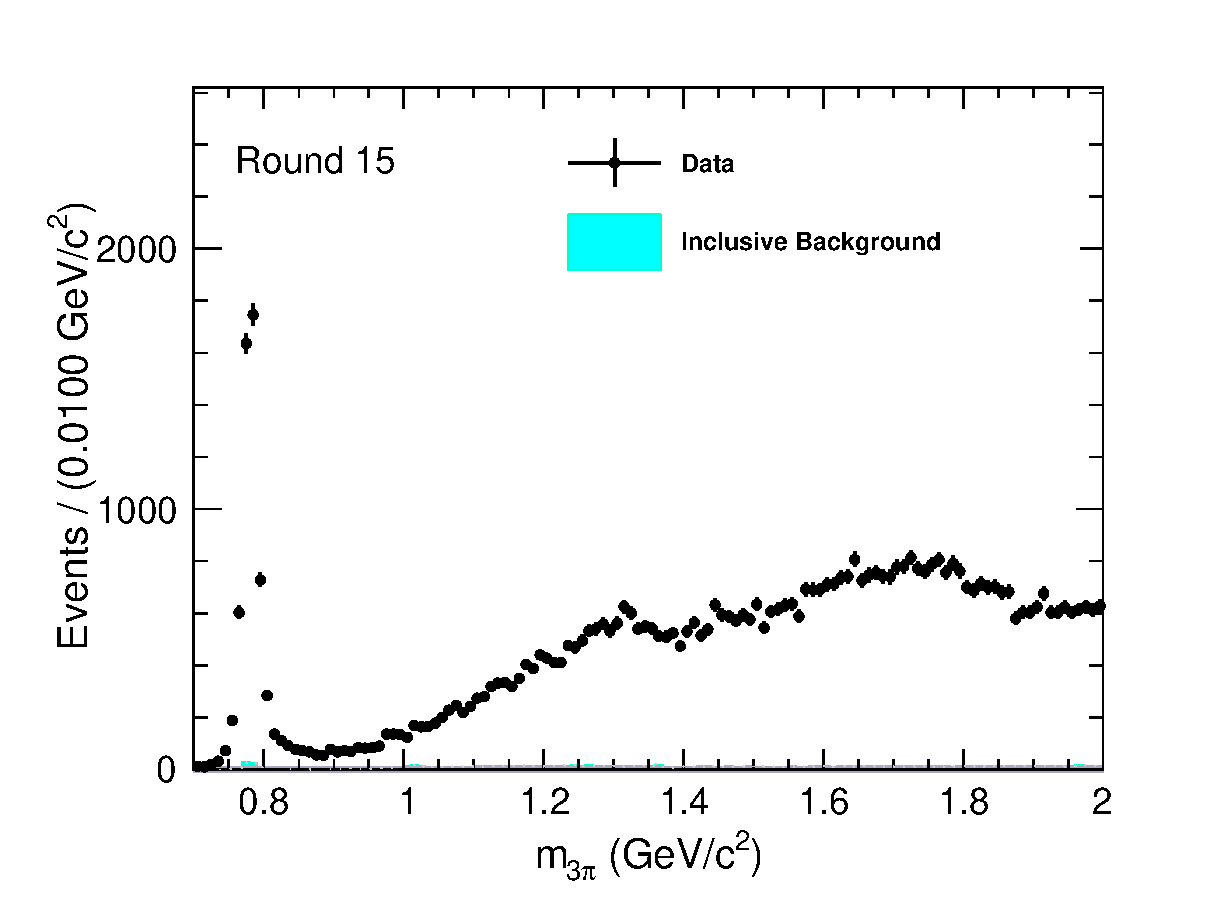
\includegraphics[width=0.40\textwidth]{fig/4pi_3pi_mass_round15.eps}
        \label{fig:4pi_background_spectrum_round15}
    }
    \\
    \subfloat[Round 16]{
        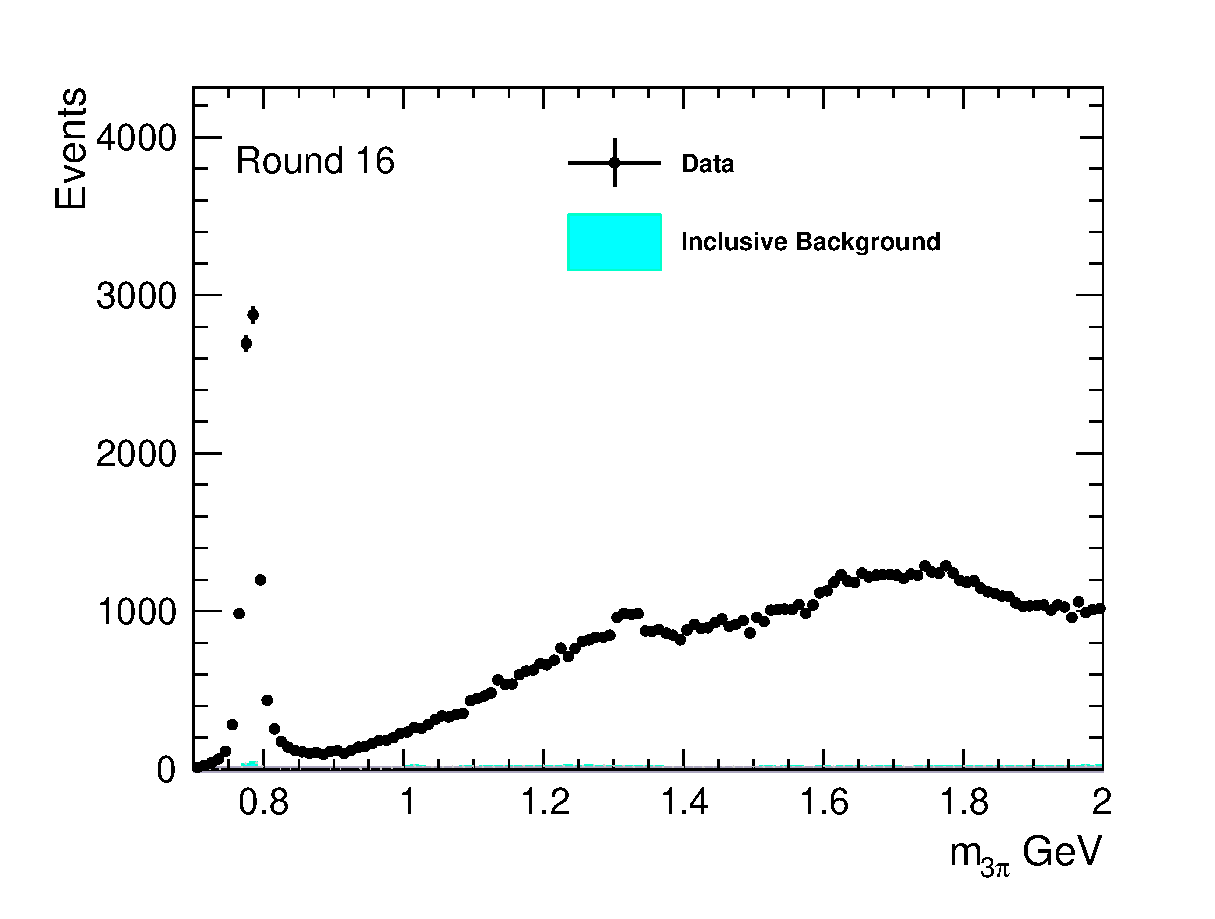
\includegraphics[width=0.40\textwidth]{fig/4pi_3pi_mass_round16.eps}
        \label{fig:4pi_background_spectrum_round16}
    }
    \hfill
    \subfloat[Round 17]{
        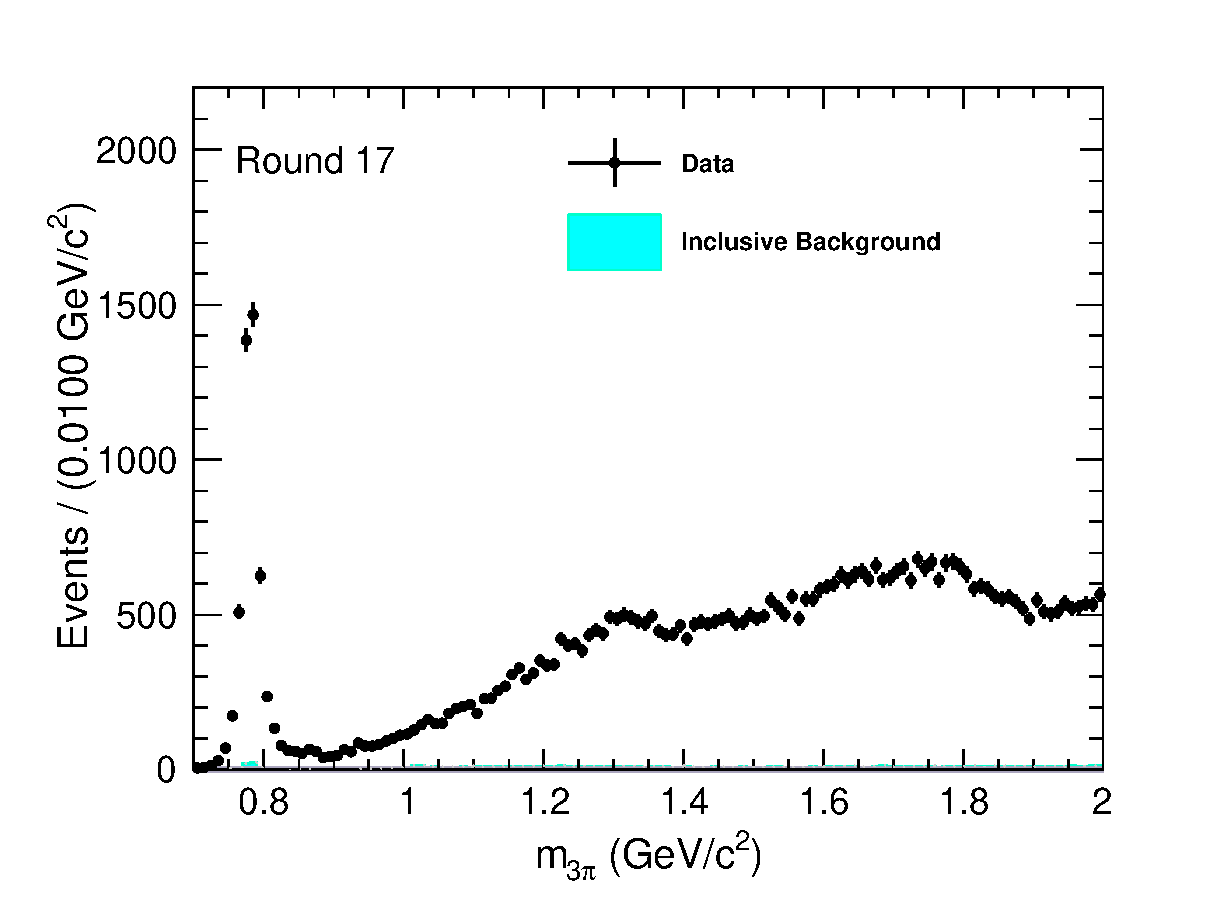
\includegraphics[width=0.40\textwidth]{fig/4pi_3pi_mass_round17.eps}
        \label{fig:4pi_background_spectrum_round17}
    }
    \caption{The $3\pi$ invariant mass spectrum from selected $e^{+}e^{-} \to \pi^{+}\pi^{-}\pi^{0}\pi^{0}$ events in the (a) Round~03/04, (b) Round~15, (c) Round~16, and (d) Round~17 datasets. These distributions, obtained from data after applying the dual-tag selection criteria for $e^{+}e^{-} \to \pi^{+}\pi^{-}\pi^{0}\pi^{0}$, represent the pure signal samples used as templates for background estimation.}
    \label{fig:4pi_background_spectrum}
\end{figure}

The observed distribution in the data, after applying the $e^{+}e^{-} \to
    \pi^{+}\pi^{-}\pi^{0}\pi^{0}$ selection criteria, will be scaled by the
efficiency ratio $R = \epsilon_{\text{bkg}} / \epsilon_{\text{sig}}$ to
estimate the final background contribution of this process in the signal region
of the measurement channel. As established and shown in
Fig.~\ref{fig:4pi_background_spectrum}, the background contamination within
this selected sample is negligible. Therefore, we subtract the inclusive
background histogram from the data histogram in a symbolic manner to obtain the
pure $e^{+}e^{-} \to \pi^{+}\pi^{-}\pi^{0}\pi^{0}$ event yield. The resulting
background-subtracted signal distributions in the three $3\pi$ invariant mass
regions are presented in Fig.~\ref{fig:nonisr4pi_all_rounds_regions}. All other
backgrounds will be subtracted directly.

% 添加结果图（四个物理区域，四个数据周期）
\begin{figure}[htbp]
\centering

% === Row 1: Round 03/04 ===
\subfloat[Round 03/04, $\omega(782)$ region]{
    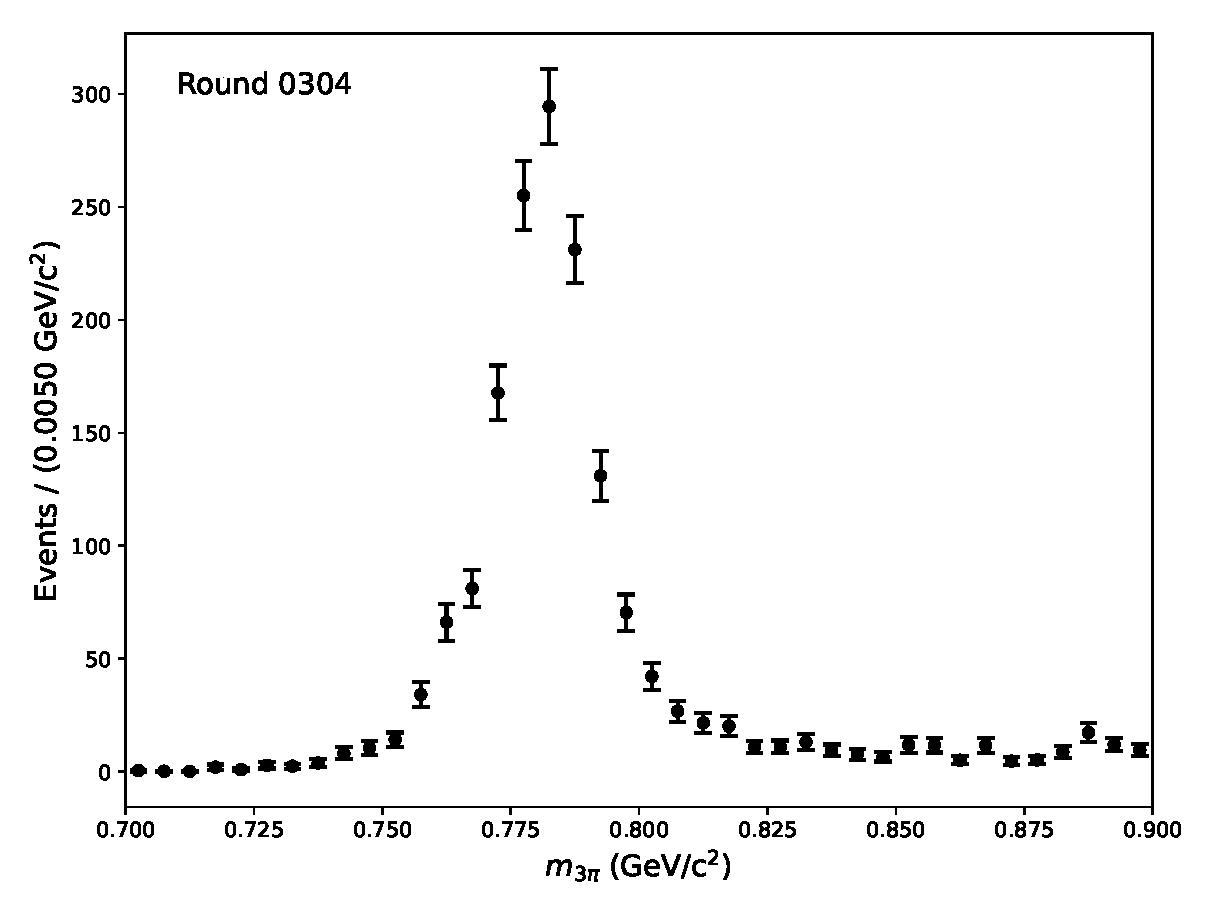
\includegraphics[width=0.32\textwidth]{fig/nonisr4pi_round0304_region1_plot.eps}
    \label{fig:nonisr4pi_r0304_region1}
}\hfill
\subfloat[Round 03/04, $\phi(1020)$ region]{
    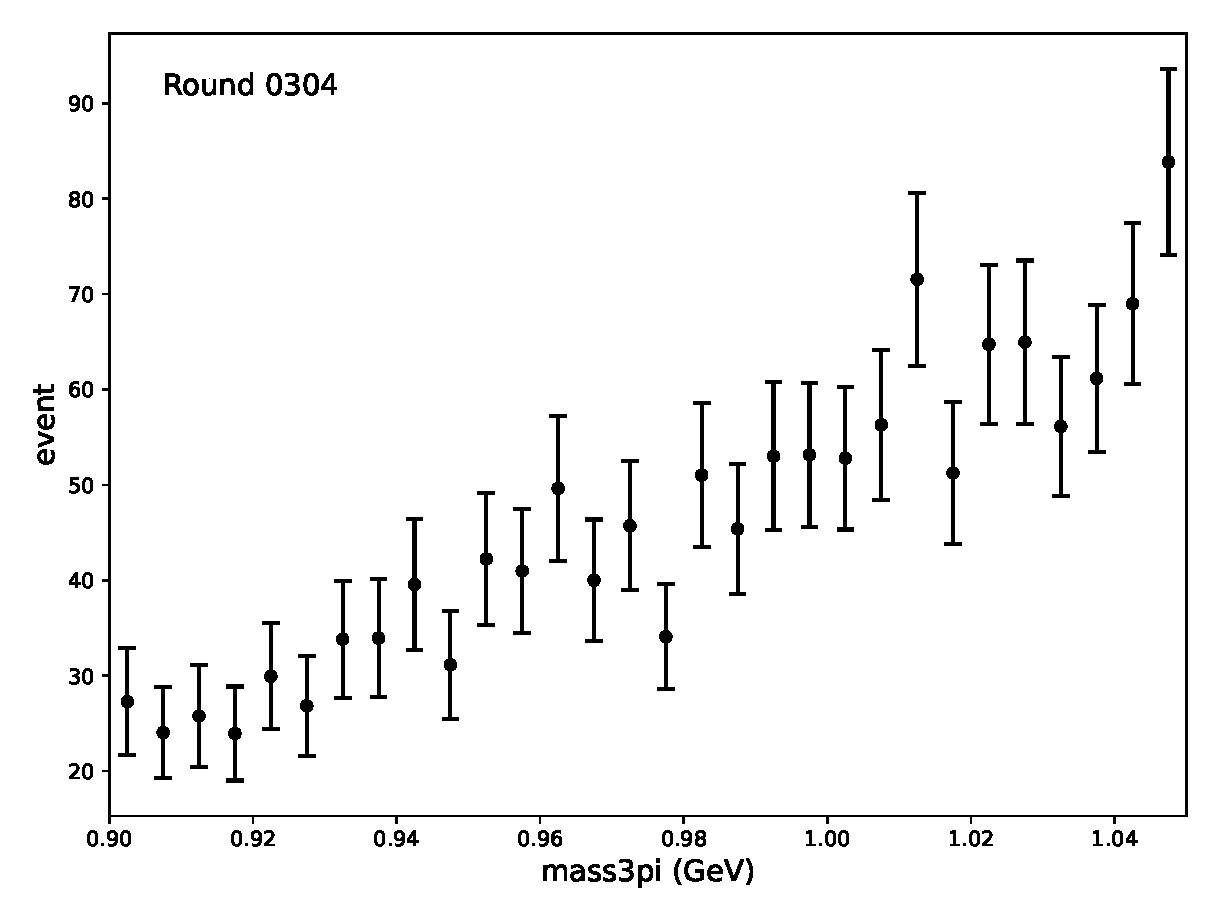
\includegraphics[width=0.32\textwidth]{fig/nonisr4pi_round0304_region2_plot.eps}
    \label{fig:nonisr4pi_r0304_region2}
}\hfill
\subfloat[Round 03/04, $\omega^{\prime}/\omega^{\prime\prime}$ region]{
    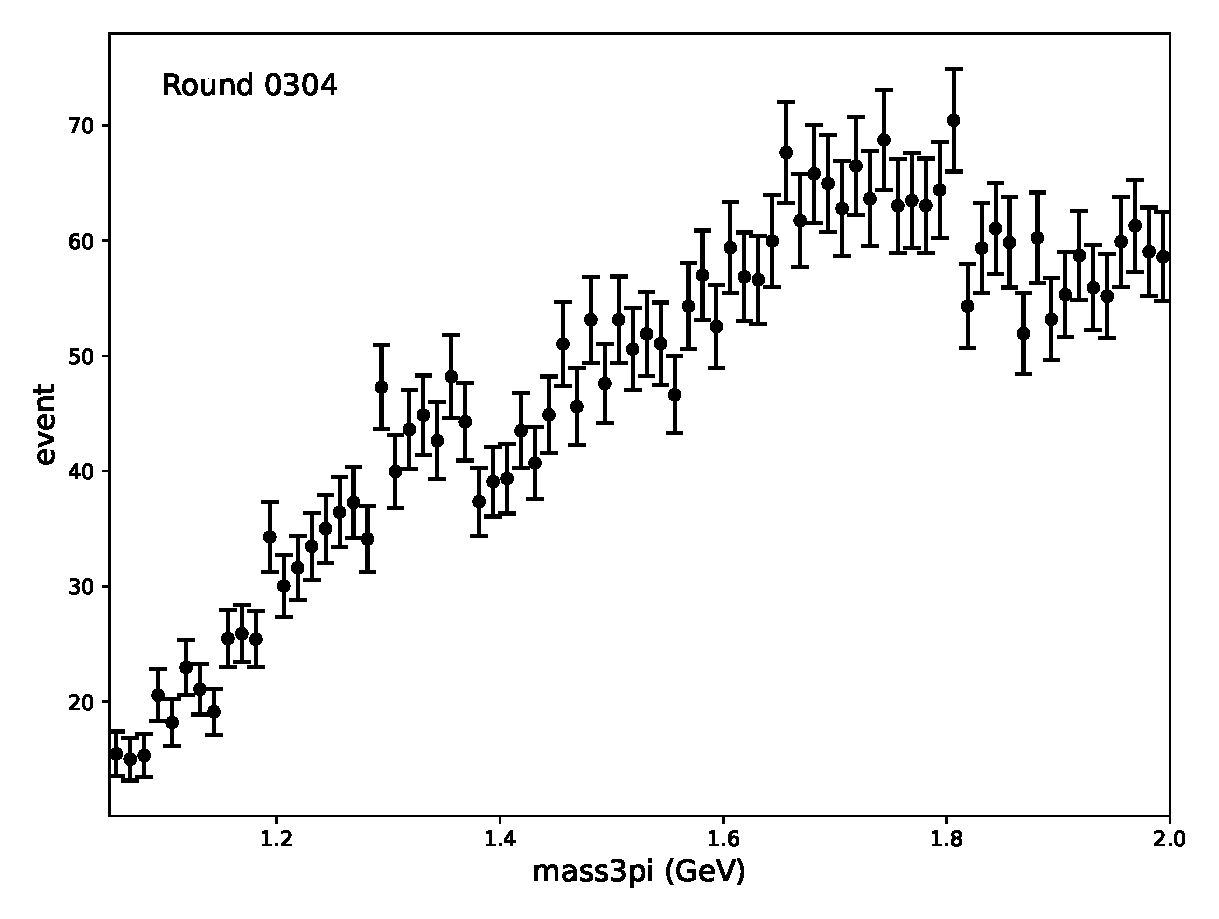
\includegraphics[width=0.32\textwidth]{fig/nonisr4pi_round0304_region3_plot.eps}
    \label{fig:nonisr4pi_r0304_region3}
}

\vspace{0.5\baselineskip}

% === Row 2: Round 15 ===
\subfloat[Round 15, $\omega(782)$ region]{
    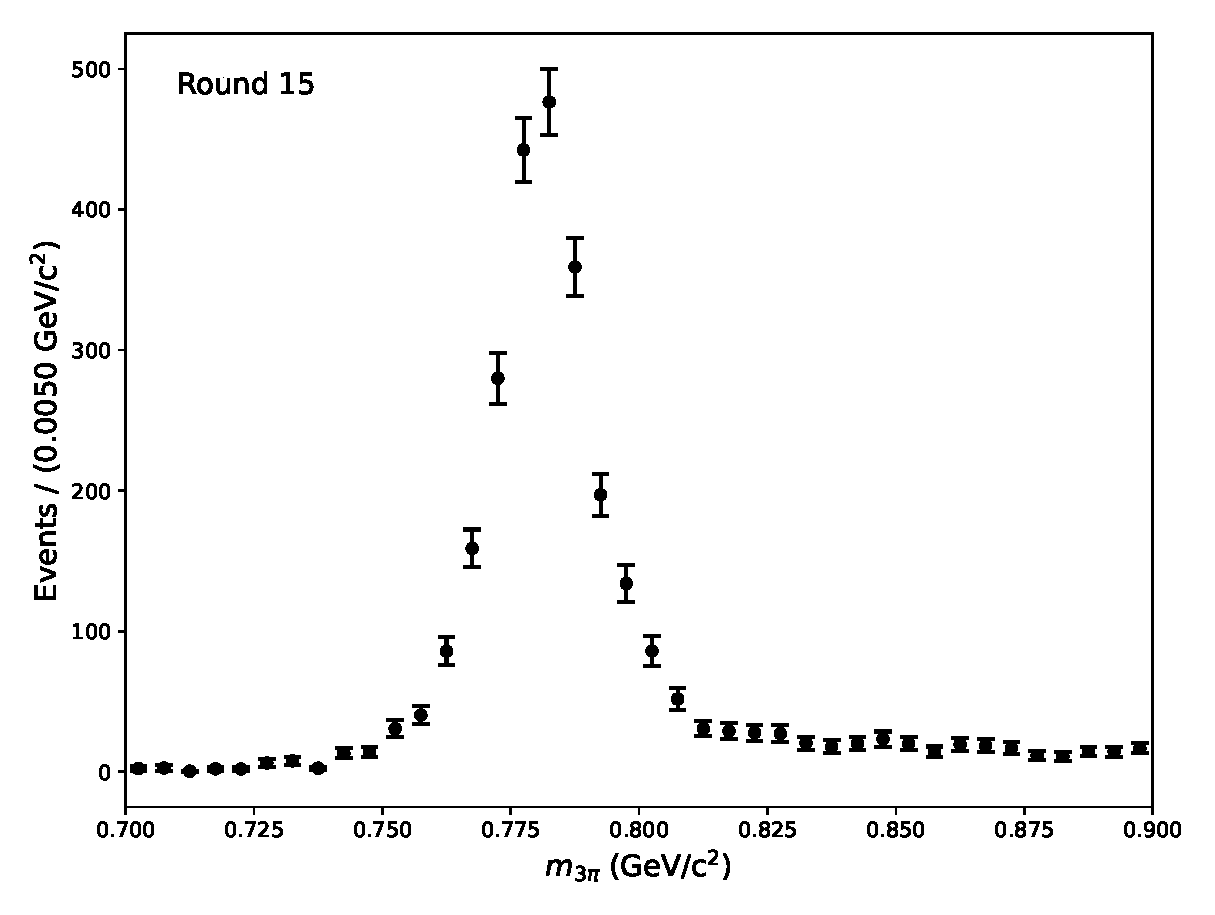
\includegraphics[width=0.32\textwidth]{fig/nonisr4pi_round15_region1_plot.eps}
    \label{fig:nonisr4pi_r15_region1}
}\hfill
\subfloat[Round 15, $\phi(1020)$ region]{
    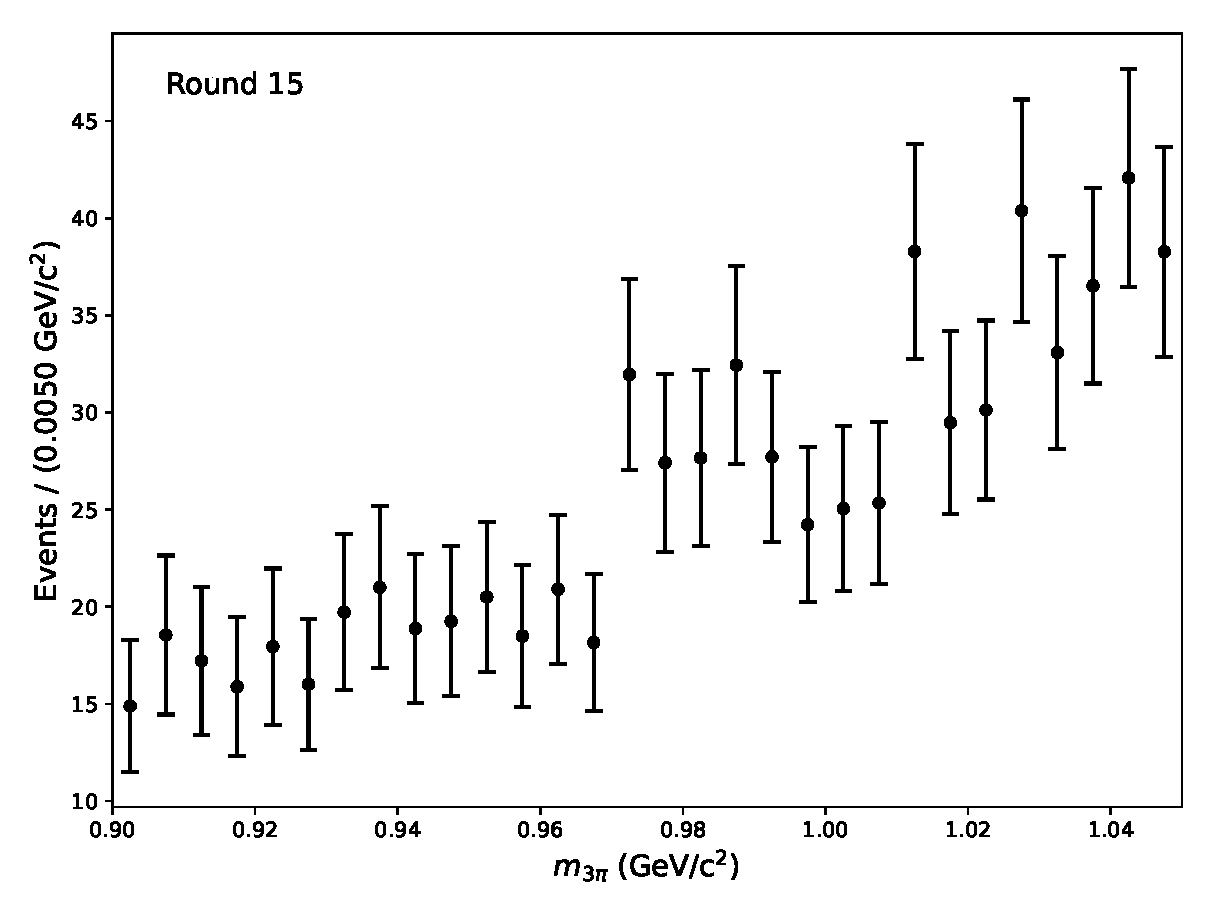
\includegraphics[width=0.32\textwidth]{fig/nonisr4pi_round15_region2_plot.eps}
    \label{fig:nonisr4pi_r15_region2}
}\hfill
\subfloat[Round 15, $\omega^{\prime}/\omega^{\prime\prime}$ region]{
    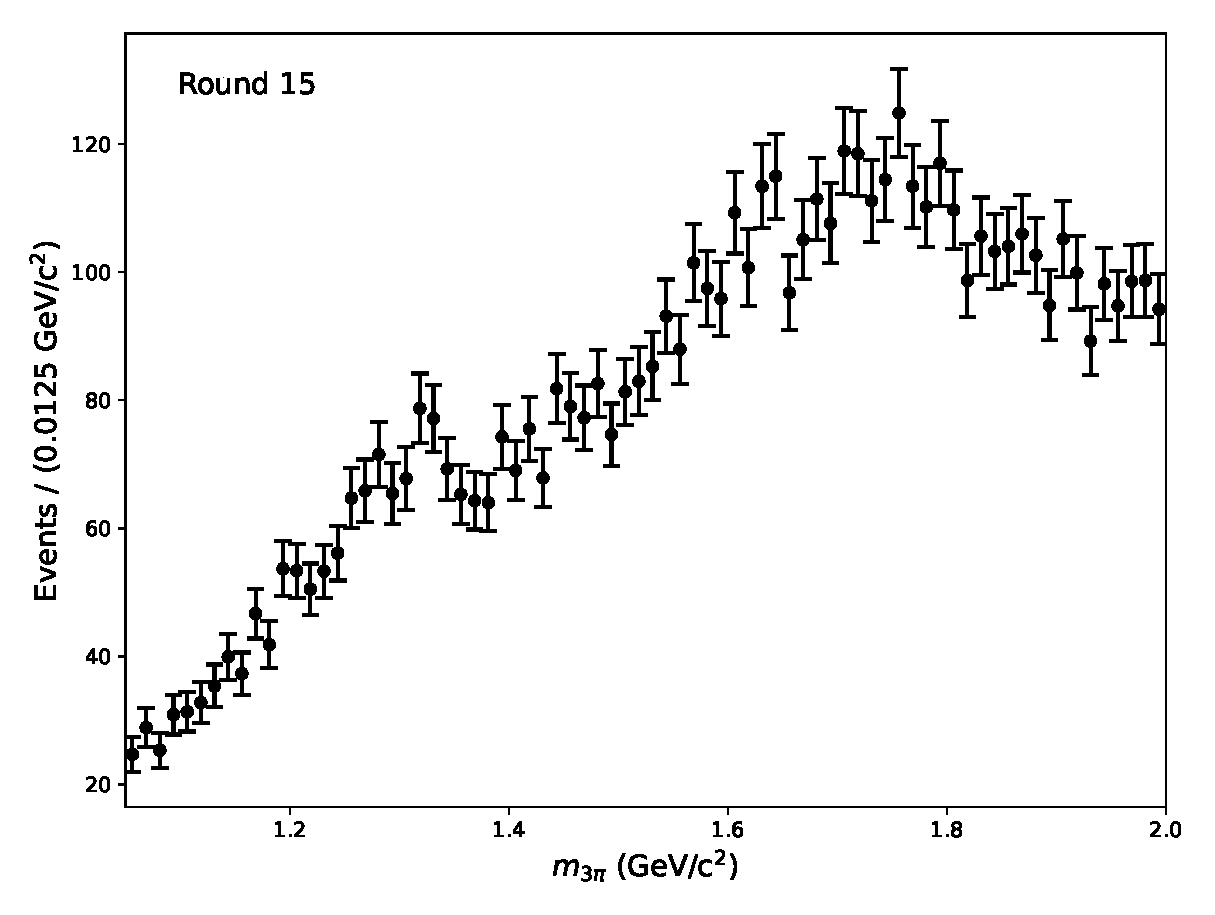
\includegraphics[width=0.32\textwidth]{fig/nonisr4pi_round15_region3_plot.eps}
    \label{fig:nonisr4pi_r15_region3}
}

\vspace{0.5\baselineskip}

% === Row 3: Round 16 ===
\subfloat[Round 16, $\omega(782)$ region]{
    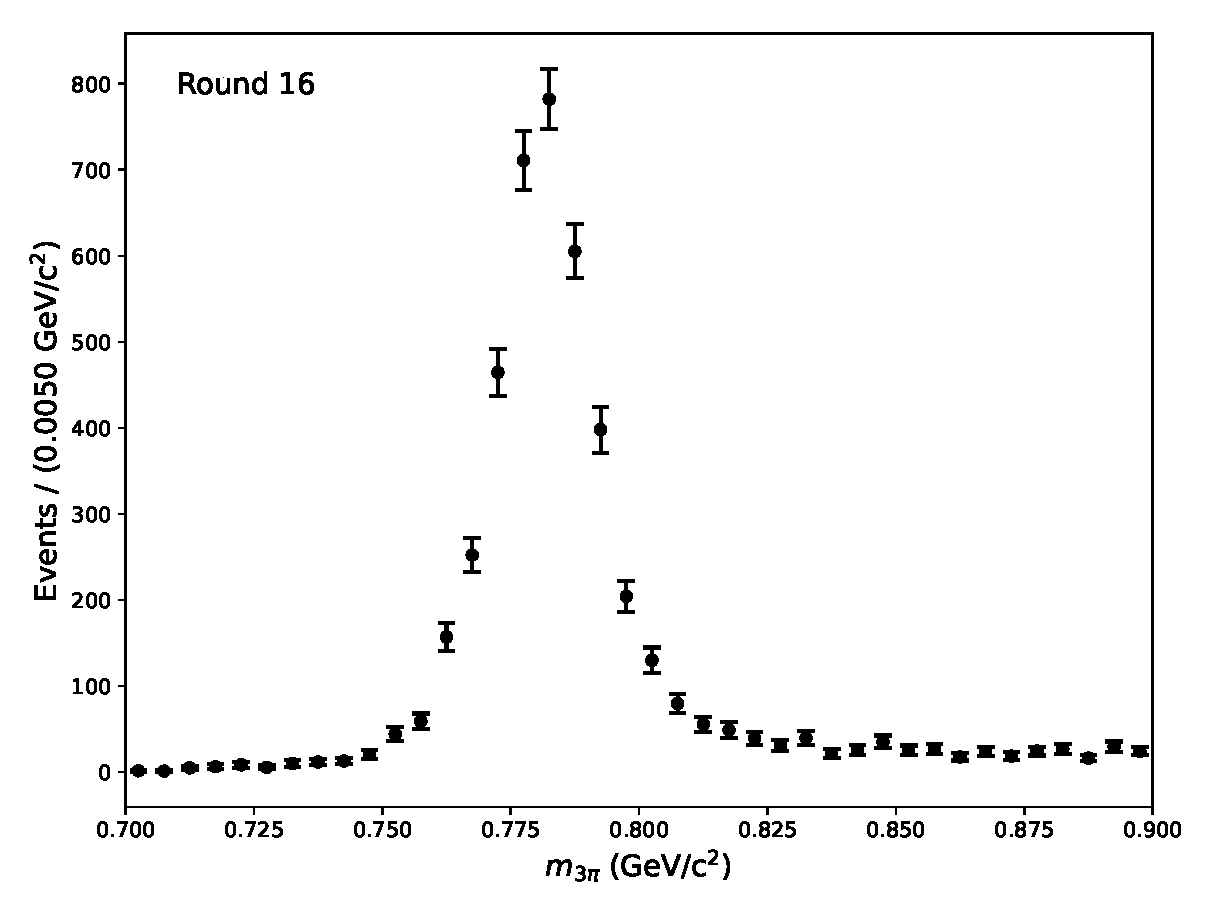
\includegraphics[width=0.32\textwidth]{fig/nonisr4pi_round16_region1_plot.eps}
    \label{fig:nonisr4pi_r16_region1}
}\hfill
\subfloat[Round 16, $\phi(1020)$ region]{
    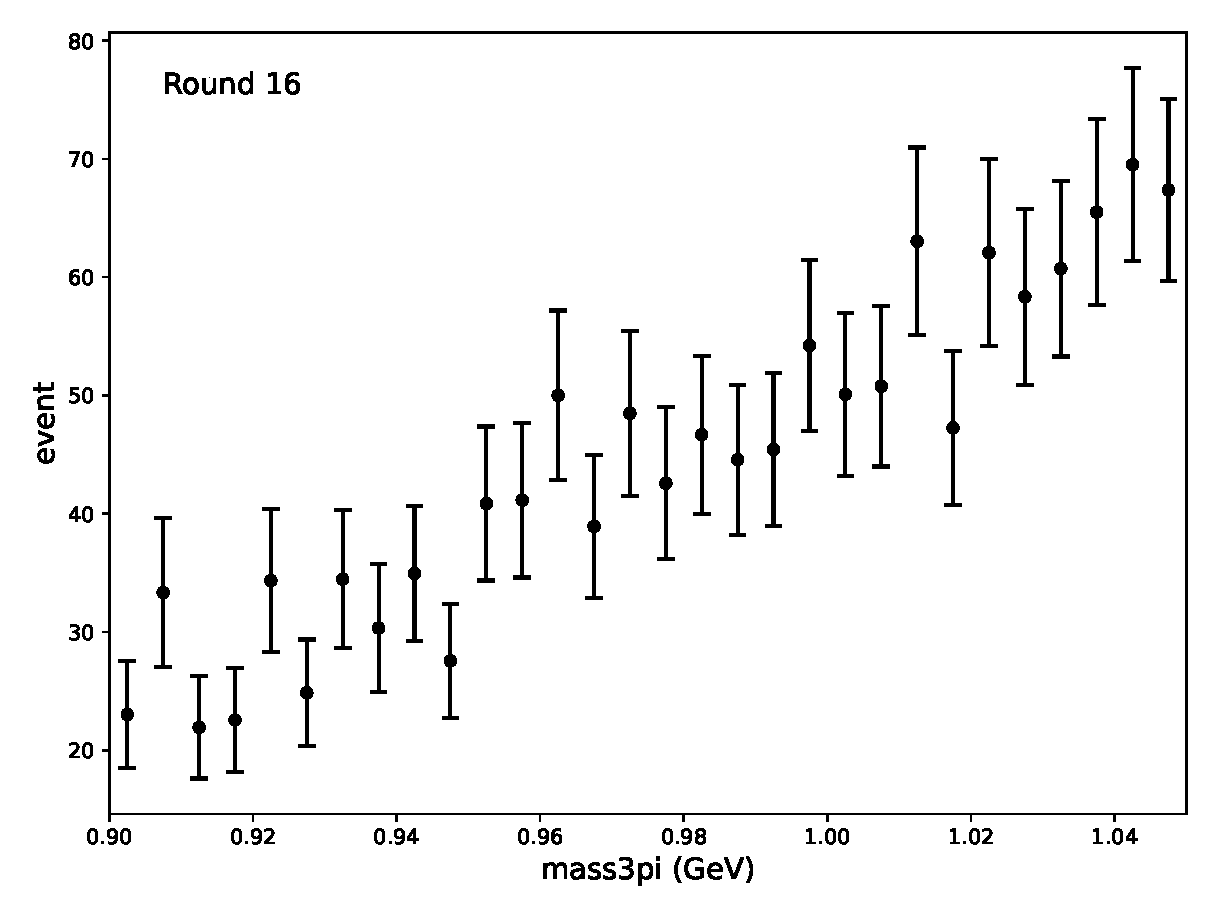
\includegraphics[width=0.32\textwidth]{fig/nonisr4pi_round16_region2_plot.eps}
    \label{fig:nonisr4pi_r16_region2}
}\hfill
\subfloat[Round 16, $\omega^{\prime}/\omega^{\prime\prime}$ region]{
    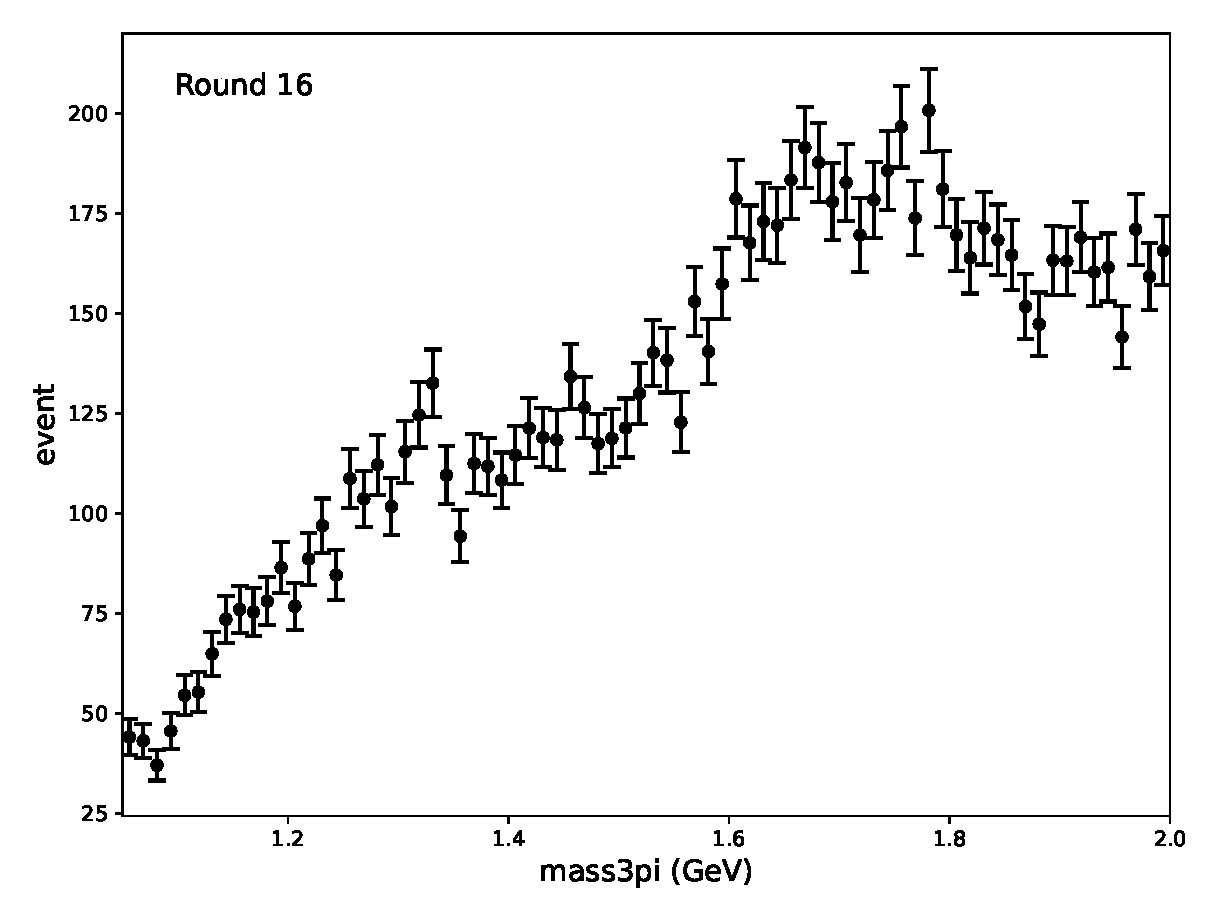
\includegraphics[width=0.32\textwidth]{fig/nonisr4pi_round16_region3_plot.eps}
    \label{fig:nonisr4pi_r16_region3}
}

\vspace{0.5\baselineskip}

% === Row 4: Round 17 ===
\subfloat[Round 17, $\omega(782)$ region]{
    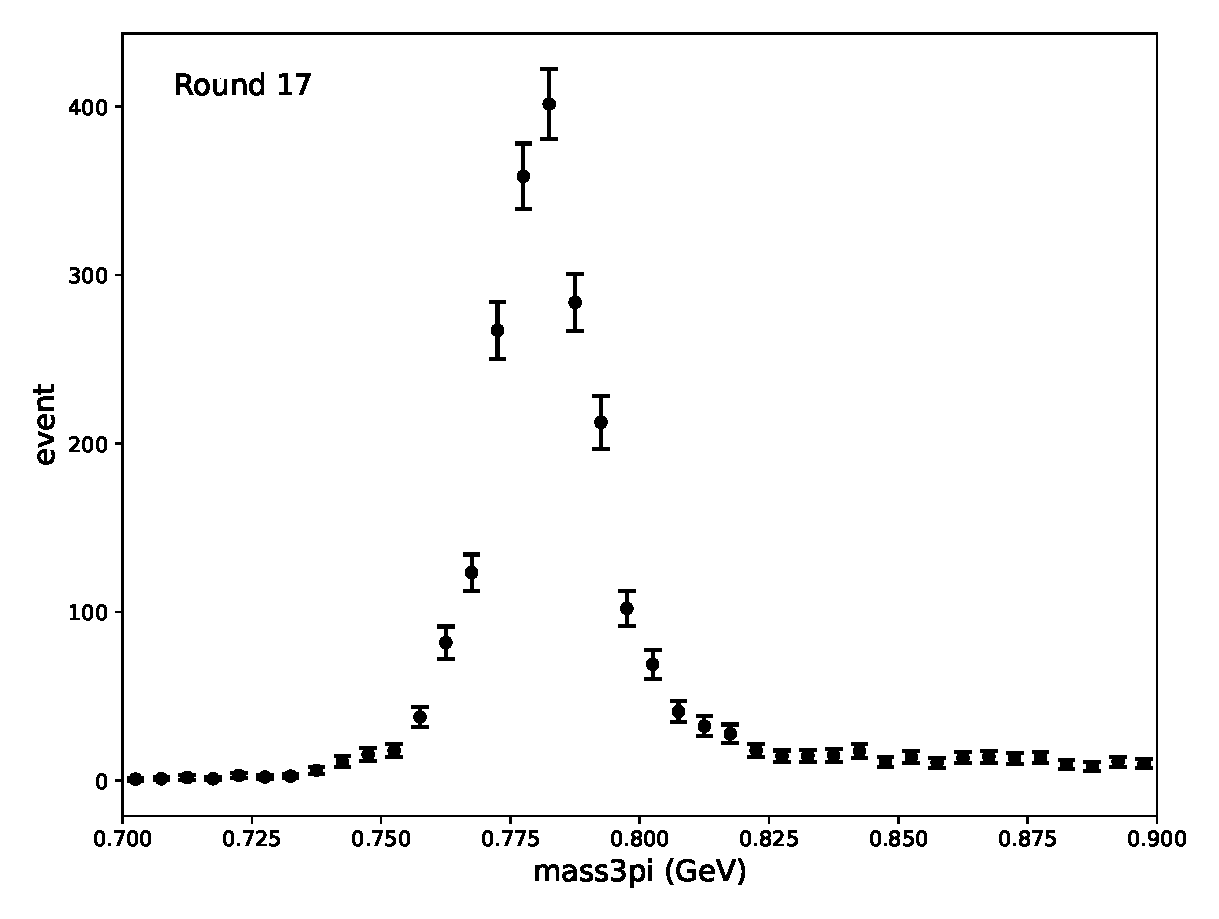
\includegraphics[width=0.32\textwidth]{fig/nonisr4pi_round17_region1_plot.eps}
    \label{fig:nonisr4pi_r17_region1}
}\hfill
\subfloat[Round 17, $\phi(1020)$ region]{
    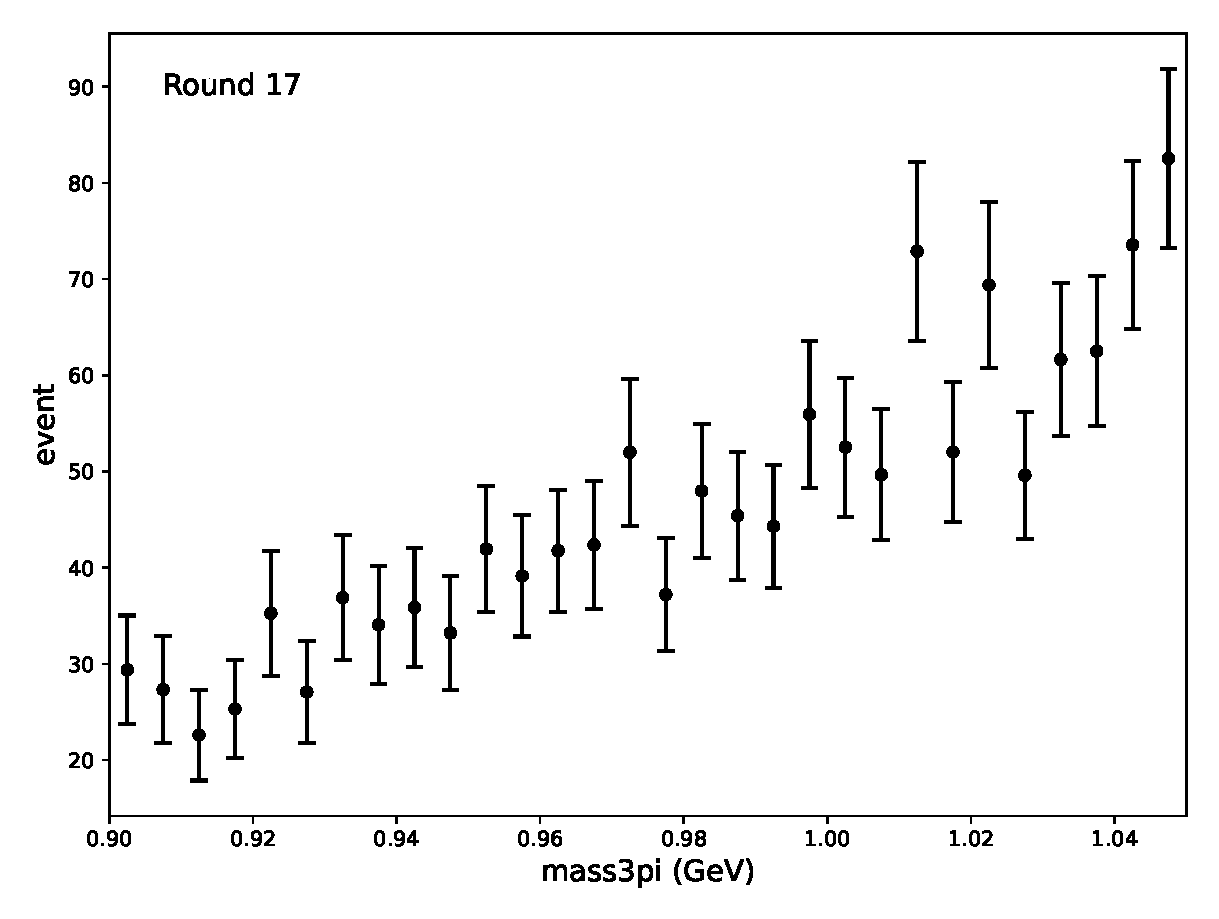
\includegraphics[width=0.32\textwidth]{fig/nonisr4pi_round17_region2_plot.eps}
    \label{fig:nonisr4pi_r17_region2}
}\hfill
\subfloat[Round 17, $\omega^{\prime}/\omega^{\prime\prime}$ region]{
    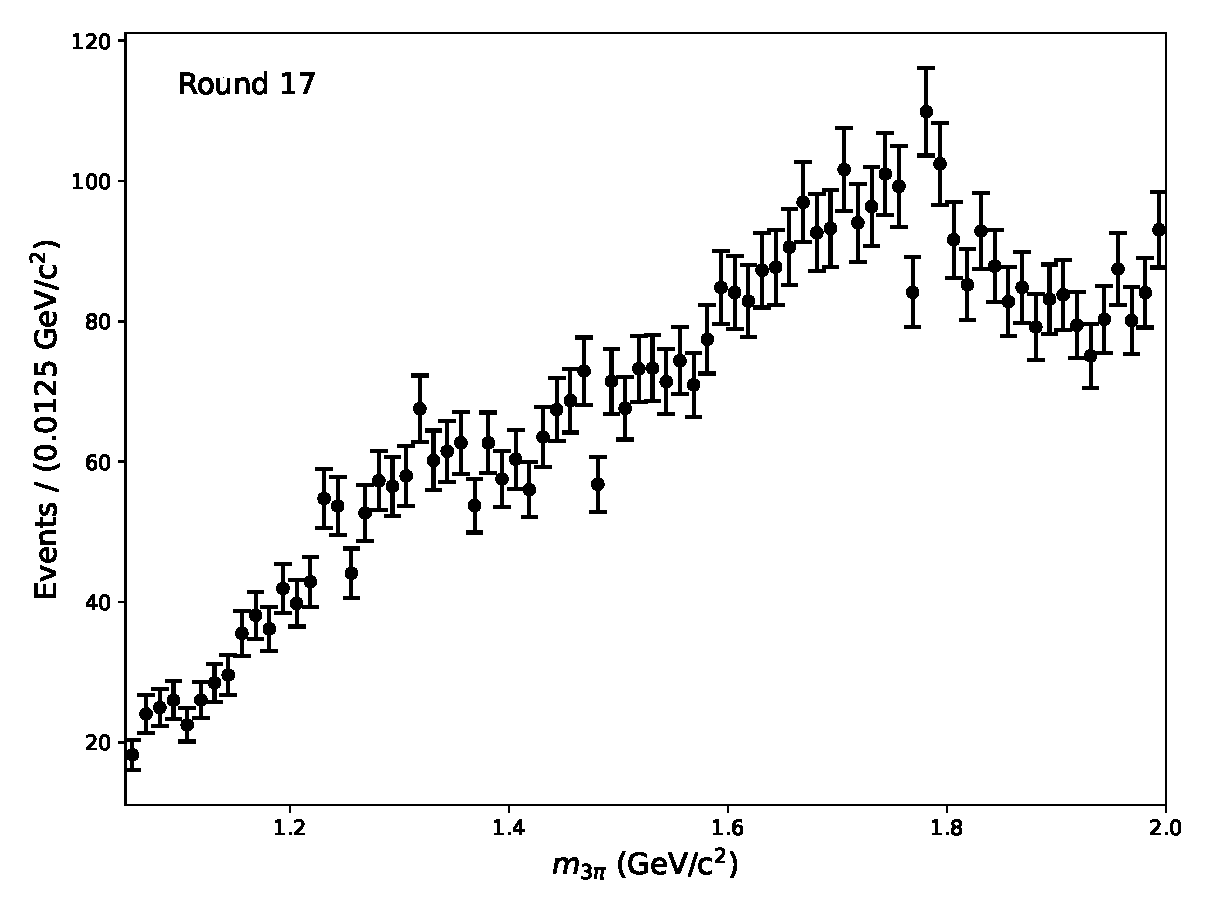
\includegraphics[width=0.32\textwidth]{fig/nonisr4pi_round17_region3_plot.eps}
    \label{fig:nonisr4pi_r17_region3}
}

\caption{Estimated background contributions from $e^{+}e^{-} \to \pi^{+}\pi^{-}\pi^{0}\pi^{0}$ in the signal region after scaling, shown for four data-taking periods. Each row corresponds to a different round: (a)--(c) Round~03/04, (d)--(f) Round~15, (g)--(i) Round~16, and (j)--(l) Round~17. The three columns represent different $3\pi$ invariant mass regions: $\omega(782)$ region (left), $\phi(1020)$ region (center), and higher-mass $\omega^{\prime}/\omega^{\prime\prime}$ region (right).}
\label{fig:nonisr4pi_all_rounds_regions}
\end{figure}

% \clearpage
% \subsection{Estimate of $\ee\to\pip\pim\piz\piz\gamma_{\text{ISR}}$}
% The second dominant background, $e^{+}e^{-} \to \gamma_{\mathrm{ISR}}\pi^{+}\pi^{-}\pi^{0}\pi^{0}$, is estimated using an analogous data-driven approach. The selection follows a similar dual-tag strategy to obtain a sample. The selection criteria are outlined below:

% Simultaneously, events must satisfy both the $e^{+}e^{-} \to \gamma_{\mathrm{ISR}}\pi^{+}\pi^{-}\pi^{0}\pi^{0}$ selection, where the $\gamma_{\mathrm{ISR}}$ is treated as an untagged missing momentum, and the tagged $e^{+}e^{-} \to \gamma_{\mathrm{ISR}}\pi^{+}\pi^{-}\pi^{0}$ loose selection criteria.

% \begin{itemize}
%     \item \textbf{$e^{+}e^{-} \to \gamma_{\mathrm{ISR}}\pi^{+}\pi^{-}\pi^{0}\pi^{0}$ Candidate Selection (Untagged $\gamma_{\mathrm{ISR}}$):}
%     \begin{itemize}
%         \item Exactly two good charged tracks.
%         \item $\text{nPi0} \geq 2$ \&\& $\text{nGoodShowers} \geq 4$ (requiring at least two $\pi^{0}$s).
%         \item The $\gamma_{\mathrm{ISR}}$ is not explicitly reconstructed from a shower. Instead, its 4-momentum is inferred as a \textit{missing} component within the kinematic fit.
%         \item A total 4-momentum constraint to the initial $e^{+}e^{-}$ collision is applied (4C fit).
%         \item The candidate with the minimum $\chi_{\mathrm{4C}}^2$ is chosen.
%         \item A requirement of $|\cos\theta_{\text{Miss}}| > 0.99$ is applied to the direction of the missing 4-momentum to ensure it is consistent with an ISR photon along the beam axis.
%         \item A kinematic fit quality cut of $\chi_{\mathrm{KF}}^2 < 10$ is applied.
%     \end{itemize}
%     \item \textbf{$\gamma_{\mathrm{ISR}}\pi^{+}\pi^{-}\pi^{0}$ Candidate Selection (within the same event):}
%     \begin{itemize}
%         \item The same two good charged tracks.
%         \item $\text{nPi0} \geq 1$ \& \& $\text{nGoodShowers} \geq 3$ (ensuring at least one $\pi^{0}$ and one photon tagged as $\gamma_{\mathrm{ISR}}$).
%         \item A total 4-momentum constraint to the initial $e^{+}e^{-}$ collision is applied (4C fit).
%         \item The candidate with the minimum $\chi_{\mathrm{4C}}^2$ is chosen.
%         \item No additional kinematic fit $\chi^2$ requirement is applied.
%     \end{itemize}
% \end{itemize}

% The application of this dual-tag selection strategy results in a highly pure sample of $e^{+}e^{-} \to \gamma_{\mathrm{ISR}}\pi^{+}\pi^{-}\pi^{0}\pi^{0}$ events. The high purity observed is a consequence of the stringent criteria. The corresponding $3\pi$ invariant mass distribution from this sample, which will be used as the input template for background estimation, is shown in Fig.~\ref{fig:isr4pi_background_spectrum}.

% \begin{figure}[htbp]
%     \centering
%     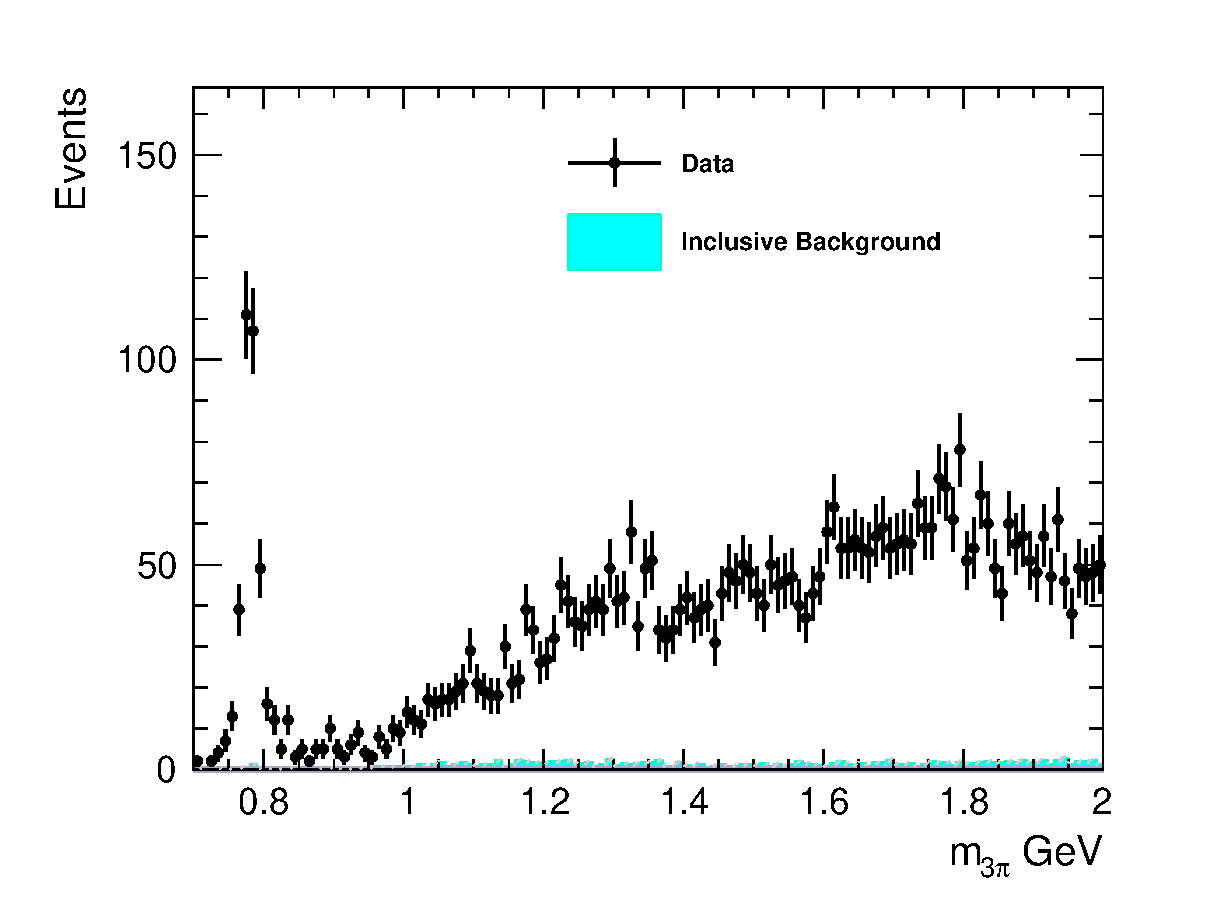
\includegraphics[width=0.45\textwidth]{fig/isr4pi_3pi_mass.eps}
%     \caption{The $3\pi$ invariant mass spectrum from selected $e^{+}e^{-} \to \gamma_{\mathrm{ISR}}\pi^{+}\pi^{-}\pi^{0}\pi^{0}$ events (green points) using data from round 16. The distribution is obtained after applying the dual-tag selection and serves as a clean template for background estimation.}
%     \label{fig:isr4pi_background_spectrum}
% \end{figure}

% As can be seen in Fig.~\ref{fig:isr4pi_background_spectrum}, the background contamination within this selected sample is negligible. Therefore, the inclusive background histogram is subtracted from the data histogram in a symbolic manner to obtain the pure $e^{+}e^{-} \to \gamma_{\mathrm{ISR}}\pi^{+}\pi^{-}\pi^{0}\pi^{0}$ event yield.

% The observed distribution will be similarly scaled by the appropriate efficiency ratio $R' = \epsilon_{\text{bkg}}' / \epsilon_{\text{sig}}'$ to estimate its contribution in the signal region. The resulting scaled background distributions in the three $3\pi$ invariant mass regions are presented in Fig.~\ref{fig:isr4pi_all_regions}.

% % 添加结果图（三个物理区域）
% \begin{figure}[htbp]
%     \centering
%     \subfloat[$\omega(782)$ region]{
%         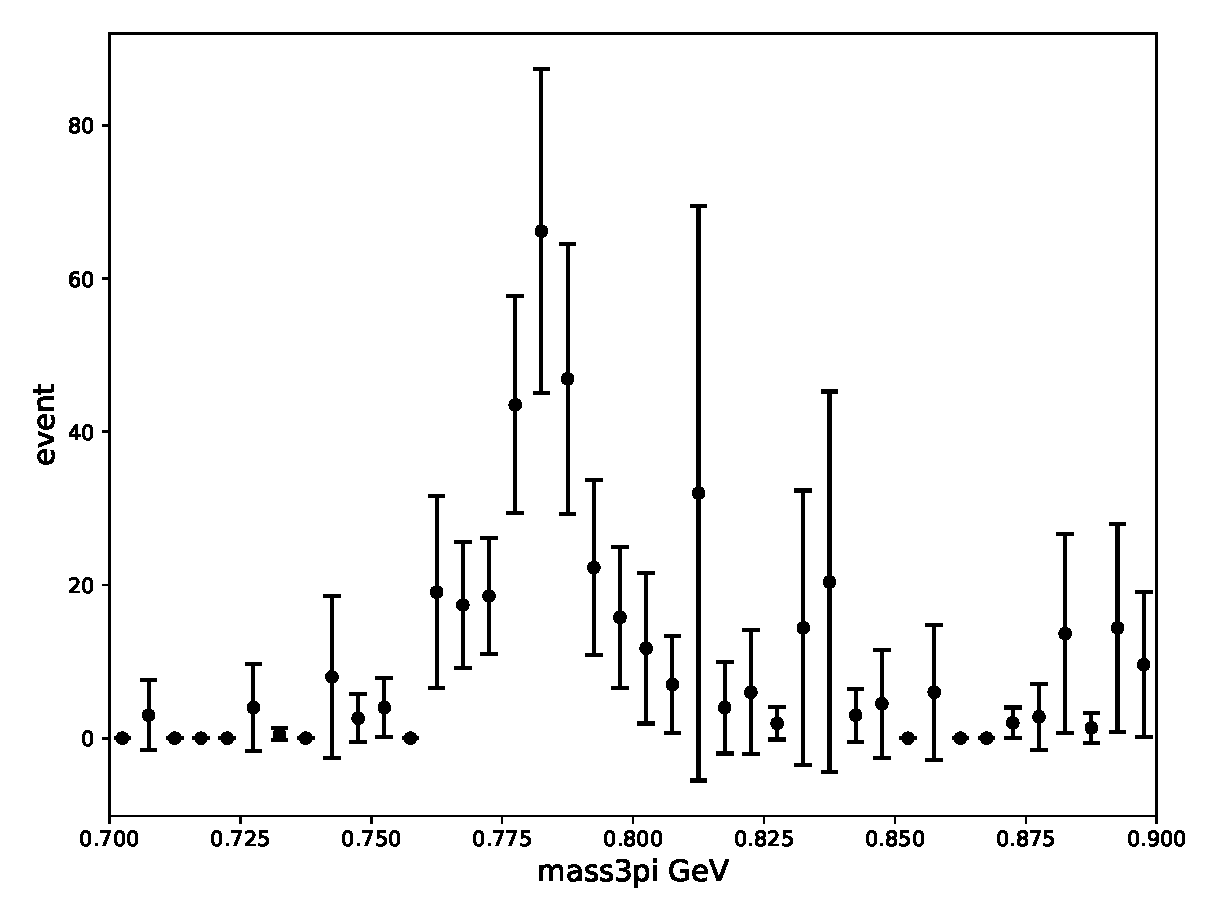
\includegraphics[width=0.32\textwidth]{fig/isr4pi_region1_plot.eps}
%         \label{fig:isr4pi_region1}
%     }
%     \hfill
%     \subfloat[$\phi(1020)$ region]{
%         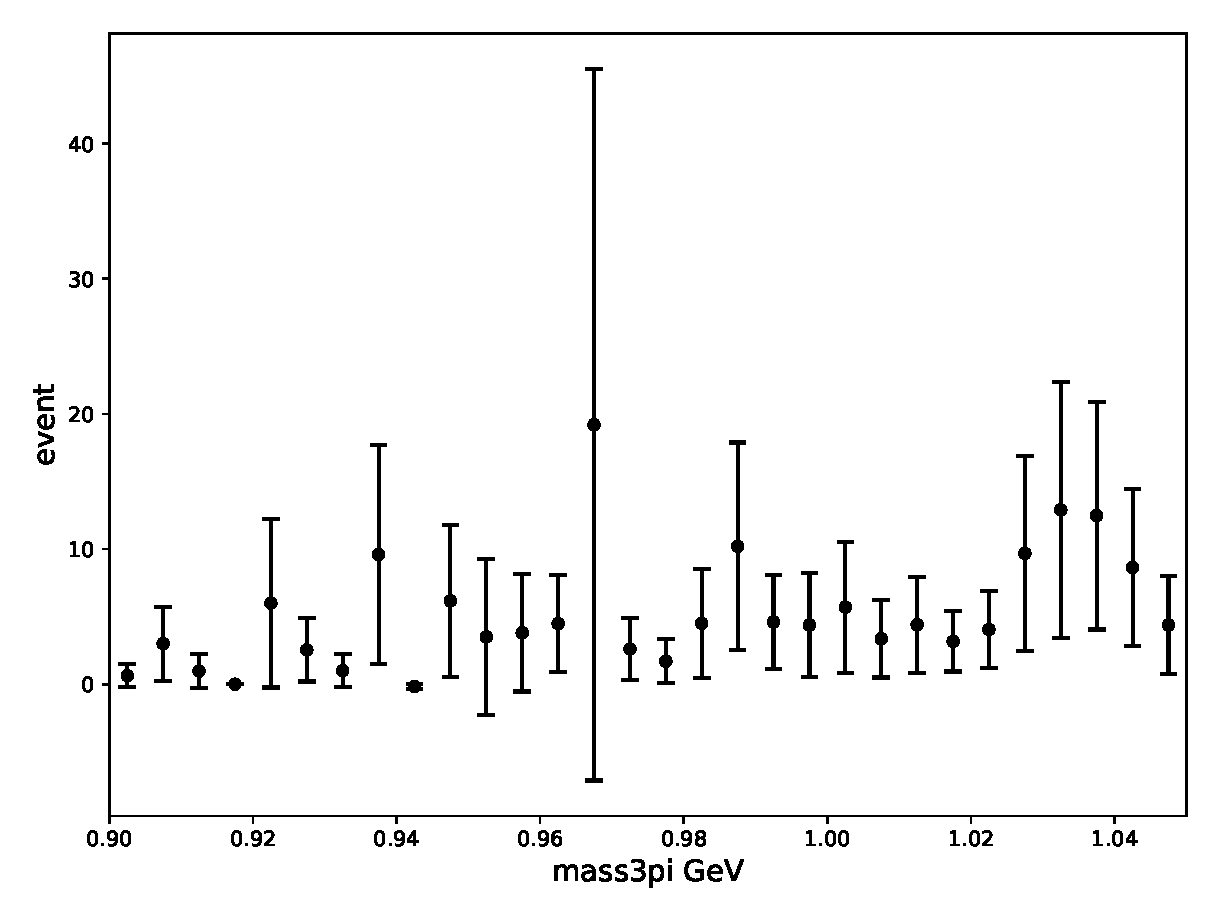
\includegraphics[width=0.32\textwidth]{fig/isr4pi_region2_plot.eps}
%         \label{fig:isr4pi_region2}
%     }
%     \hfill
%     \subfloat[$\omega^{\prime}$ and $\omega^{\prime\prime}$ region]{
%         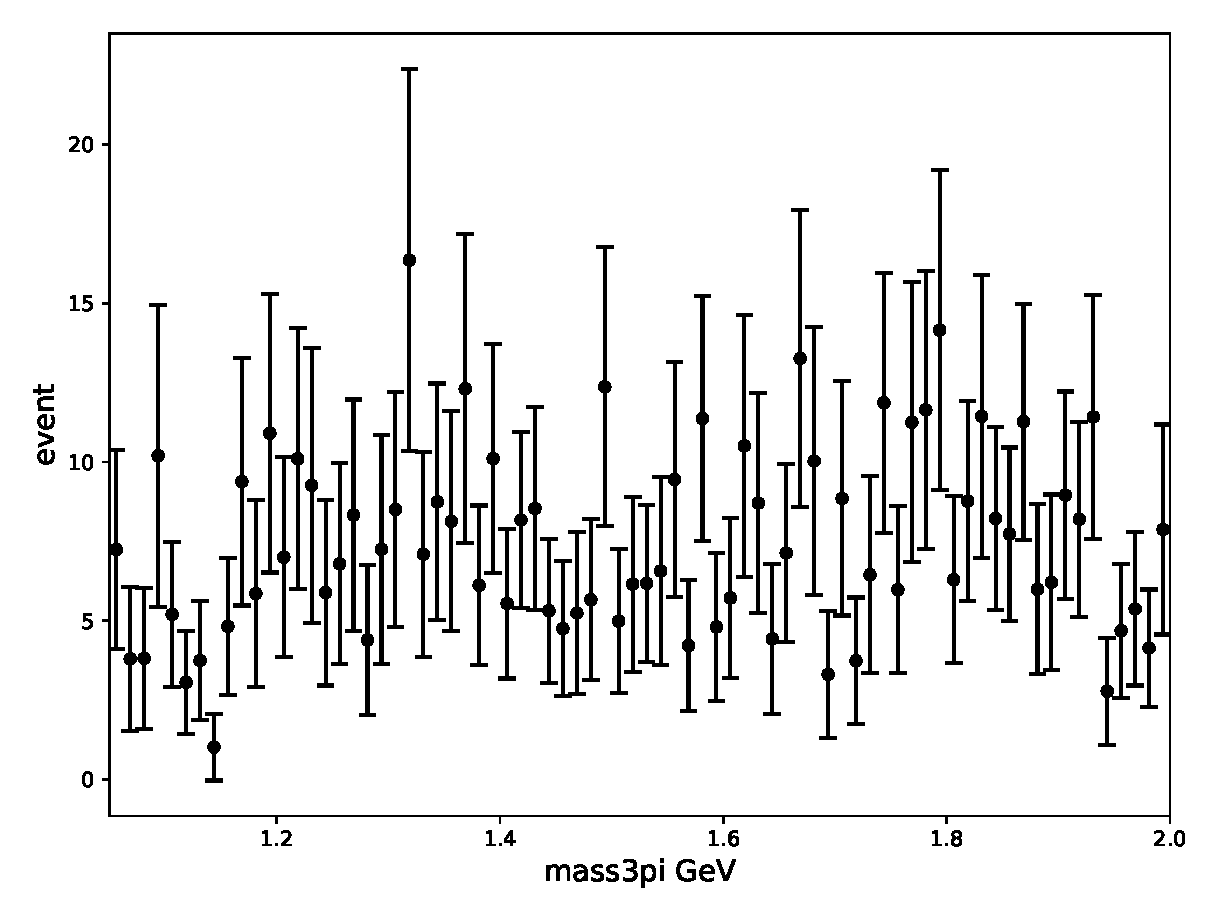
\includegraphics[width=0.32\textwidth]{fig/isr4pi_region3_plot.eps}
%         \label{fig:isr4pi_region3}
%     }
%     \caption{Estimated background contributions from $e^{+}e^{-} \to \gamma_{\mathrm{ISR}}\pi^{+}\pi^{-}\pi^{0}\pi^{0}$ in the signal region after scaling, using data from round 16. The three panels correspond to different $3\pi$ invariant mass regions: (a) the $\omega(782)$ region, (b) the $\phi(1020)$ region, and (c) the higher-mass $\omega^{\prime}/\omega^{\prime\prime}$ region.}
%     \label{fig:isr4pi_all_regions}
% \end{figure}

\clearpage
\subsection{Estimate of Other Backgrounds and Signal Yields}
\label{DataYields}
The estimation of the dominant peaking backgrounds from $e^{+}e^{-} \to
    \pi^{+}\pi^{-}\pi^{0}\pi^{0}$ has been completed in the previous subsection.
These backgrounds exhibit shapes similar to the signal resonance peaks and are
therefore categorized as peaking backgrounds.

In addition to the peaking component, a non-peaking continuum background
component must also be accounted for in the analysis. The primary objective of
this study is to measure the cross section for $e^{+}e^{-} \to
    \pi^{+}\pi^{-}\pi^{0}$ via ISR. The ISR photon reduces the effective c.m.
energy, allowing the measurement of the signal yield in narrow intervals of the
$3\pi$ invariant mass ($M_{3\pi}$).

The $M_{3\pi}$ spectrum is divided into three physically motivated regions,
each subdivided into multiple bins for detailed study:
\begin{itemize}
    \item The $\omega(782)$ region ($0.7$–$0.9~\text{GeV}/c^{2}$), divided into 40 bins.
    \item The $\phi(1020)$ region ($0.9$–$1.05~\text{GeV}/c^{2}$), divided into 30 bins.
    \item The $\omega^{\prime}/\omega^{\prime\prime}$ region
          ($1.05$–$2.0~\text{GeV}/c^{2}$), divided into 76 bins.
\end{itemize}

For each small $M_{3\pi}$ interval, the signal yield is extracted through an
extended unbinned maximum-likelihood fit to the $U_{\text{miss}}$ distribution,
where $U_{\text{miss}}$ is defined as the difference between the missing energy
and the magnitude of the missing momentum ($U_{\text{miss}} = E_{\text{miss}} -
    |\vec{p}_{\text{miss}}|$). The fit model incorporates probability density
functions (PDFs) representing the signal and all background components.

To illustrate the composition of $U_{\text{miss}}$ distributions across
different $M_{3\pi}$ regions, the inclusive MC simulation is examined.
Figure~\ref{fig:inclusiveMC_umiss_examples} shows the $U_{\text{miss}}$
distributions for the full $\omega(782)$ region, the full $\phi(1020)$ region,
and the full $\omega^{\prime}/\omega^{\prime\prime}$ region respectively, with
the peaking background contribution from $e^{+}e^{-} \to
    \pi^{+}\pi^{-}\pi^{0}\pi^{0}$ stacked according to its expected yield. These
distributions demonstrate the characteristic features of each mass region that
motivate our fitting strategy.

\begin{figure}[htbp]
    \centering
    \subfloat[$\omega(782)$ region]{
        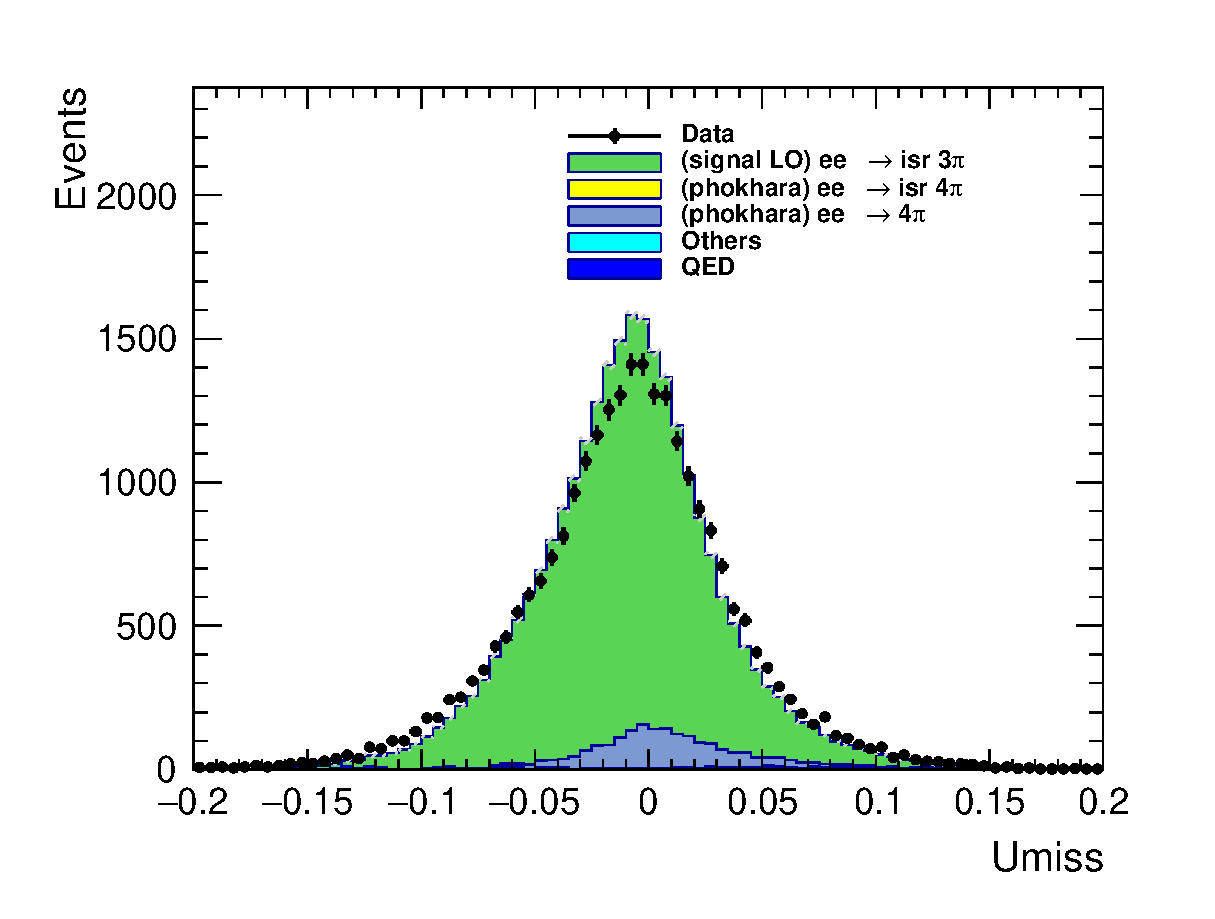
\includegraphics[width=0.32\textwidth]{fig/umiss_inclusiveMC_low.eps}
        \label{fig:umiss_inclusiveMC_low}
    }
    \hfill
    \subfloat[$\phi(1020)$ region]{
        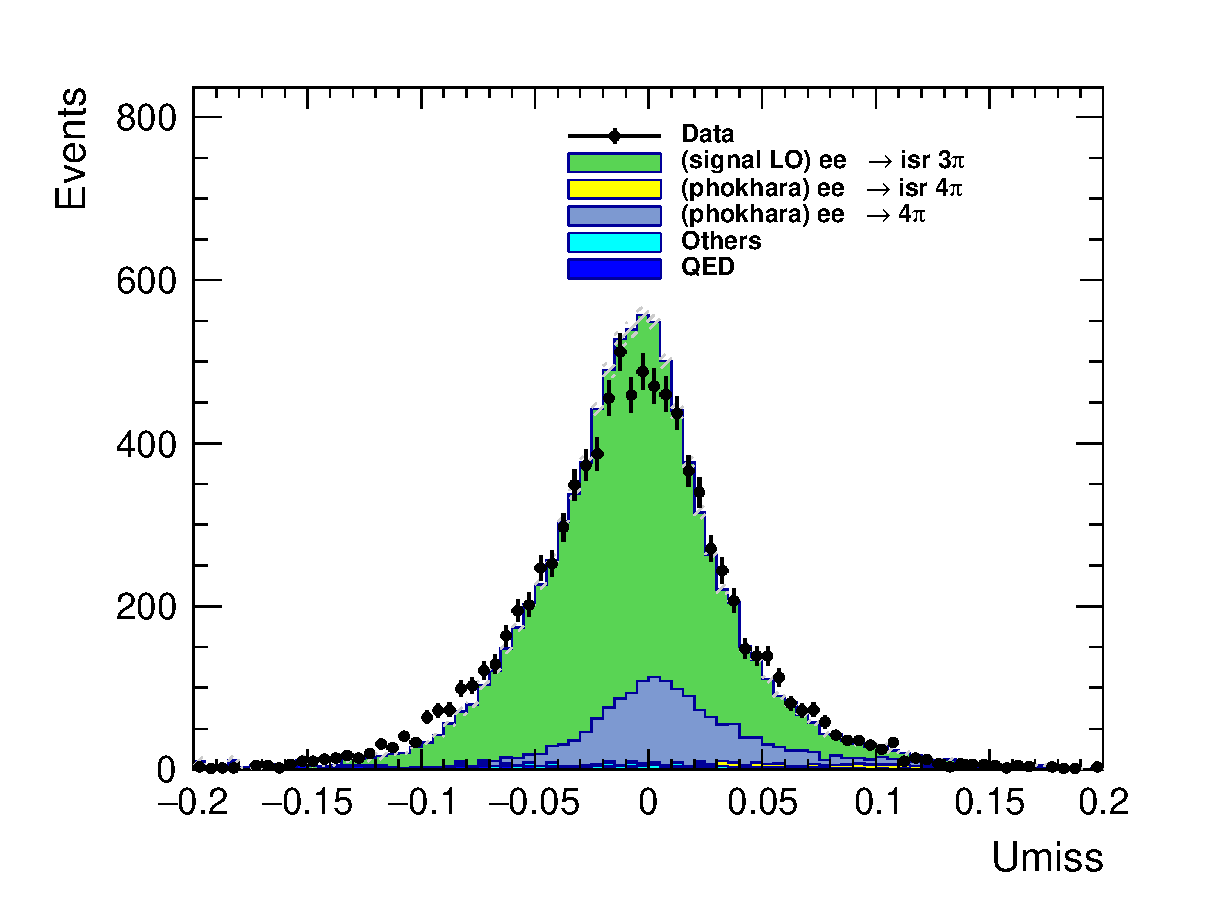
\includegraphics[width=0.32\textwidth]{fig/umiss_inclusiveMC_medium.eps}
        \label{fig:umiss_inclusiveMC_medium}
    }
    \hfill
    \subfloat[$\omega^{\prime}$ and $\omega^{\prime\prime}$ region]{
        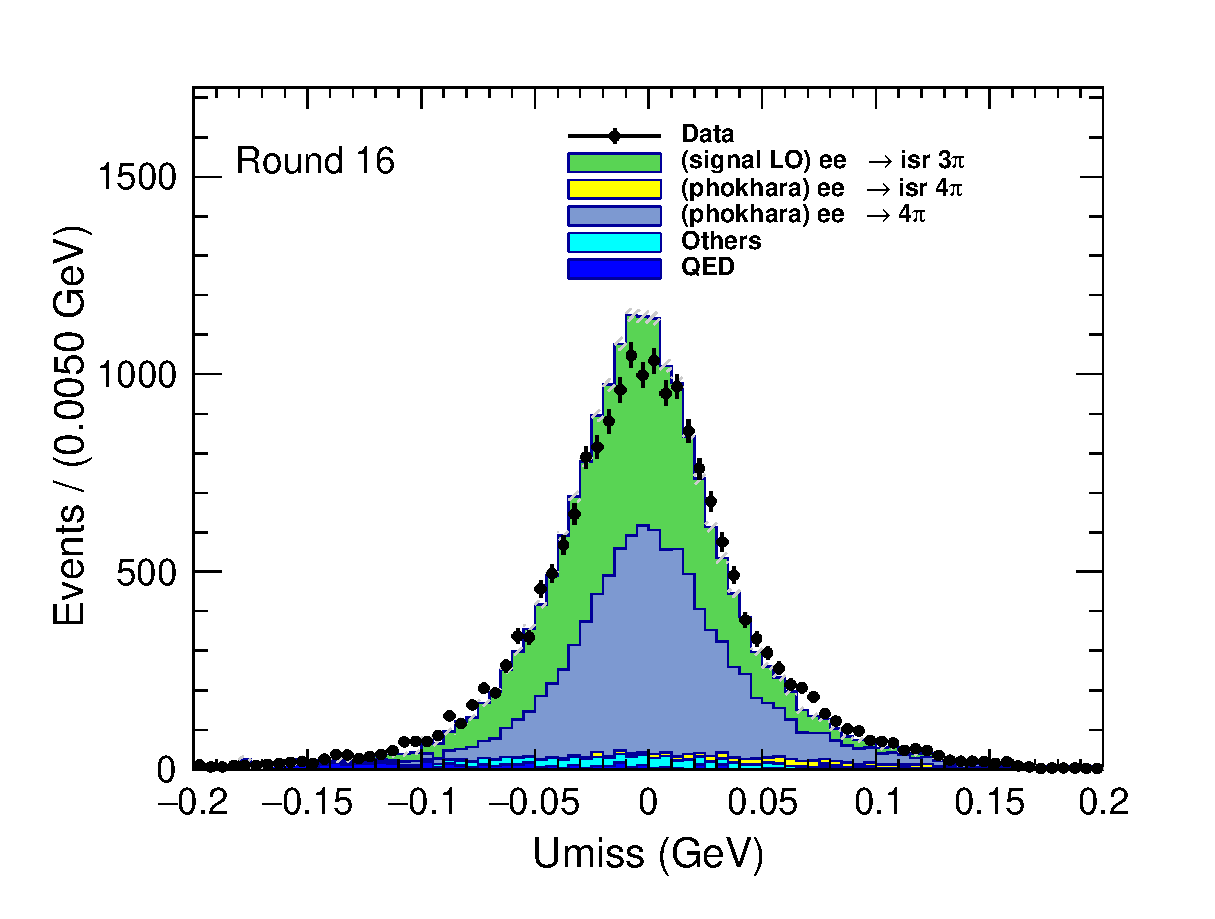
\includegraphics[width=0.32\textwidth]{fig/umiss_inclusiveMC_high.eps}
        \label{fig:umiss_inclusiveMC_high}
    }
    \caption{$U_{\text{miss}}$ distributions from inclusive MC simulation for three $M_{3\pi}$ regions: (a) the $\omega(782)$ region, (b) the $\phi(1020)$ region, and (c) the higher-mass $\omega^{\prime}/\omega^{\prime\prime}$ region.}
    \label{fig:inclusiveMC_umiss_examples}
\end{figure}

Based on the understanding from the inclusive MC, the PDFs for the fit are
constructed as follows:

\begin{itemize}
    \item \textbf{Signal PDF:} Histogram shape from signal MC, convolved with a Gaussian for resolution correction. The $\chi^{2}_{\mathrm{KF}}$ used in the $\chi^{2}_{\mathrm{KF}} < 50$ selection criterion has been corrected for data-MC differences in helix parameters as described in Section~\ref{sec:corr_signal_kmfit}.

    \item \textbf{Peaking background PDF:} Shape for $e^{+}e^{-} \to \pi^{+}\pi^{-}\pi^{0}\pi^{0}$ from dedicated MC, convolved with the same Gaussian as signal. Yield constrained by Gaussian term using data-driven estimate from Section~\ref{sec:bkg_stu}.

    \item \textbf{PDF shape sharing across bins:} Limited MC statistics preclude bin-by-bin shape extraction. Instead:
          \begin{itemize}
              \item For the $\omega(782)$ and $\phi(1020)$ regions, where the $M_{3\pi}$ bin width
                    is 5~MeV/$c^{2}$, the PDF shapes are extracted from MC simulation every five
                    consecutive bins, corresponding to 25~MeV/$c^{2}$ intervals. All five bins
                    within each such interval share the same PDF shape, under the assumption that
                    the $U_{\text{miss}}$ distribution varies slowly over this mass range.

              \item For the $\omega^{\prime}/\omega^{\prime\prime}$ region, where the $M_{3\pi}$
                    bin width is 12.5~MeV/$c^{2}$, the PDF shapes are also extracted every
                    25~MeV/$c^{2}$. Each extracted shape is therefore shared by two adjacent bins,
                    balancing the need for shape precision against the limited MC statistics in
                    this higher-mass region.
          \end{itemize}

    \item \textbf{Continuum background PDF:} All remaining minor background processes are collectively described by a polynomial function. A first-order polynomial (linear function) is used for the $\omega(782)$ and $\phi(1020)$ regions, while a second-order Chebyshev polynomial is employed for the $\omega^{\prime}/\omega^{\prime\prime}$ region, as suggested by the shape of the inclusive MC distribution in Fig.~\ref{fig:umiss_inclusiveMC_high}.
\end{itemize}

The fit procedure is validated by examining the quality of the fits to data in representative $M_{3\pi}$ bins across the three mass regions, using Round 16 as an illustrative example. Figure~\ref{fig:fit_examples} presents typical fit results for three selected bins, one from each region, demonstrating the ability of the fit model to accurately describe the data. The signal component, peaking background from $\pi^{+}\pi^{-}\pi^{0}\pi^{0}$, and polynomial continuum background are clearly distinguished, and the total PDF provides an excellent description of the data distribution in each case.

\begin{figure}[htbp]
    \centering
    \subfloat[Example bin in the $\omega(782)$ region]{
        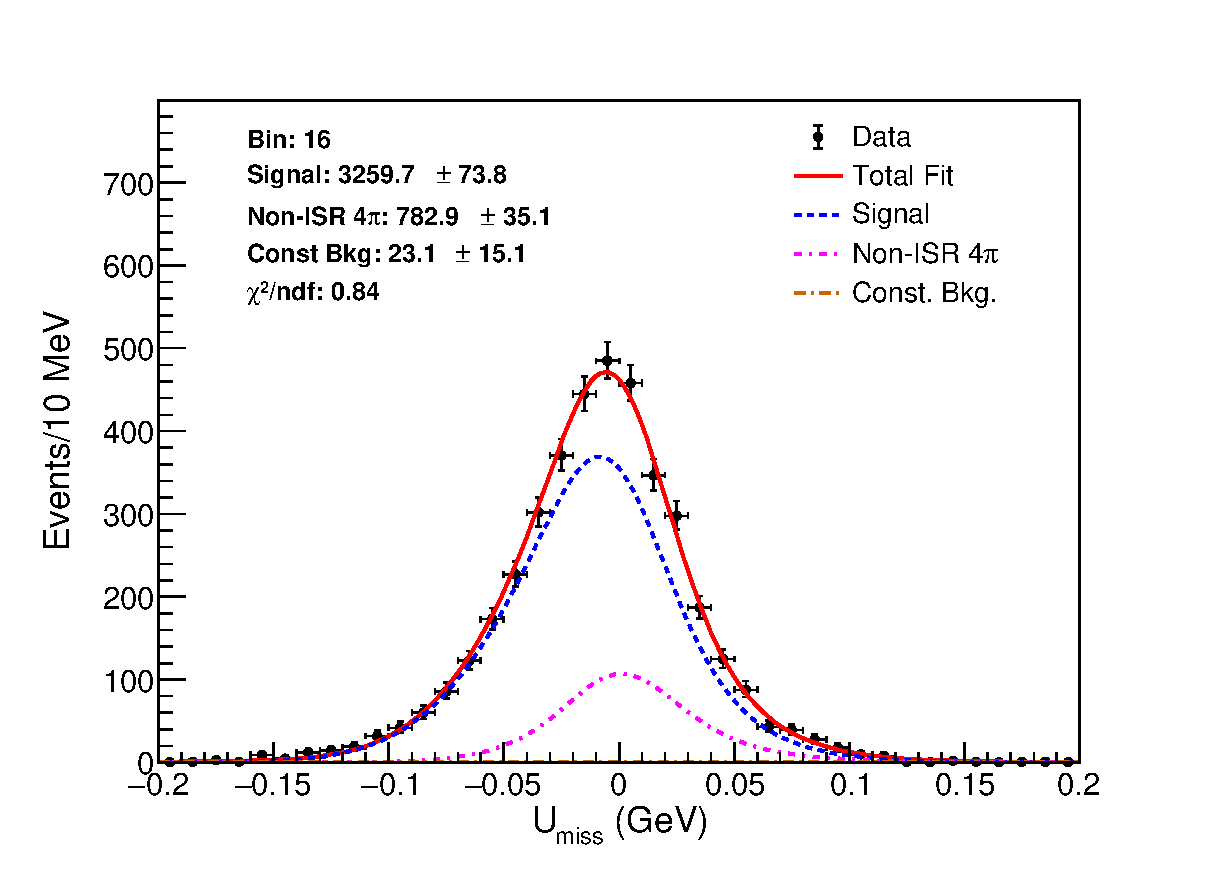
\includegraphics[width=0.32\textwidth]{fig/fit_example_omega.eps}
        \label{fig:fit_example_omega}
    }
    \hfill
    \subfloat[Example bin in the $\phi(1020)$ region]{
        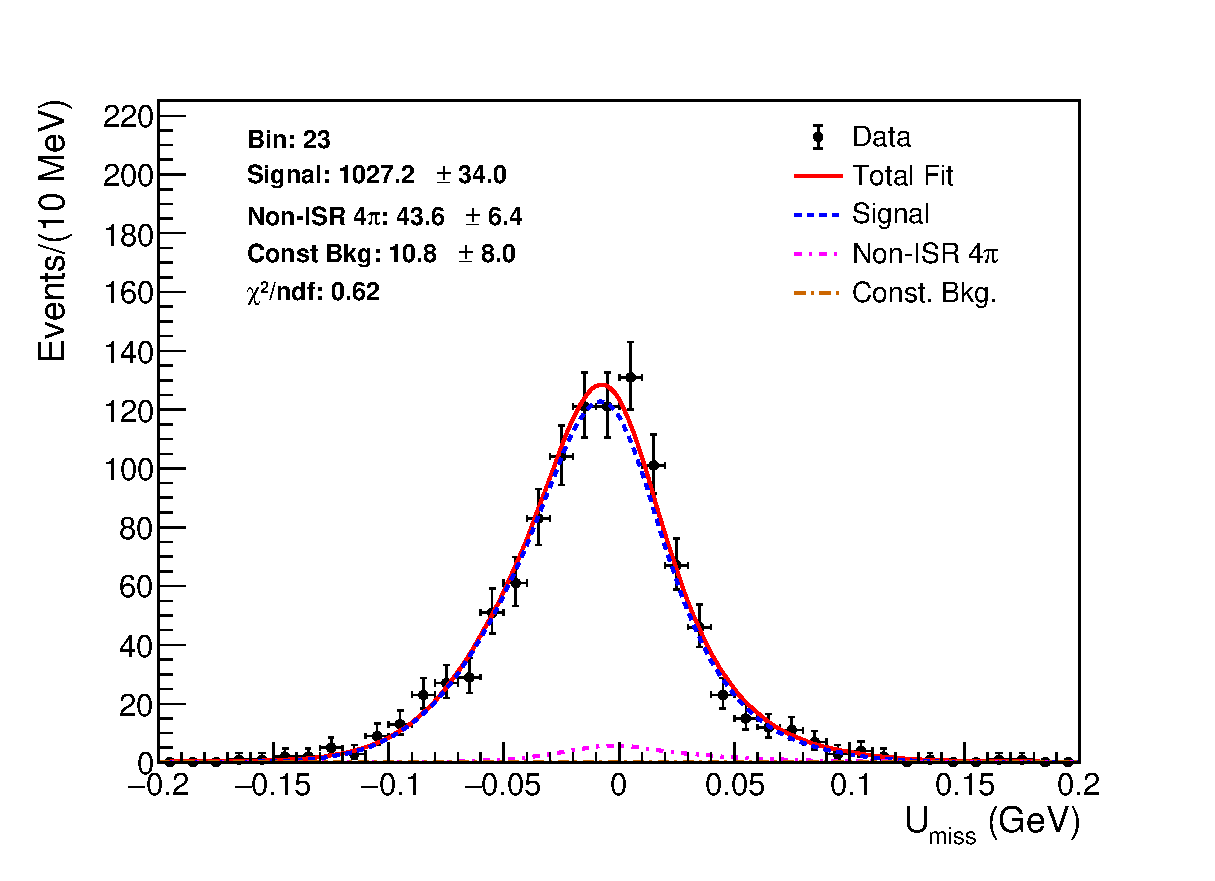
\includegraphics[width=0.32\textwidth]{fig/fit_example_phi.eps}
        \label{fig:fit_example_phi}
    }
    \hfill
    \subfloat[Example bin in the $\omega^{\prime}/\omega^{\prime\prime}$ region]{
        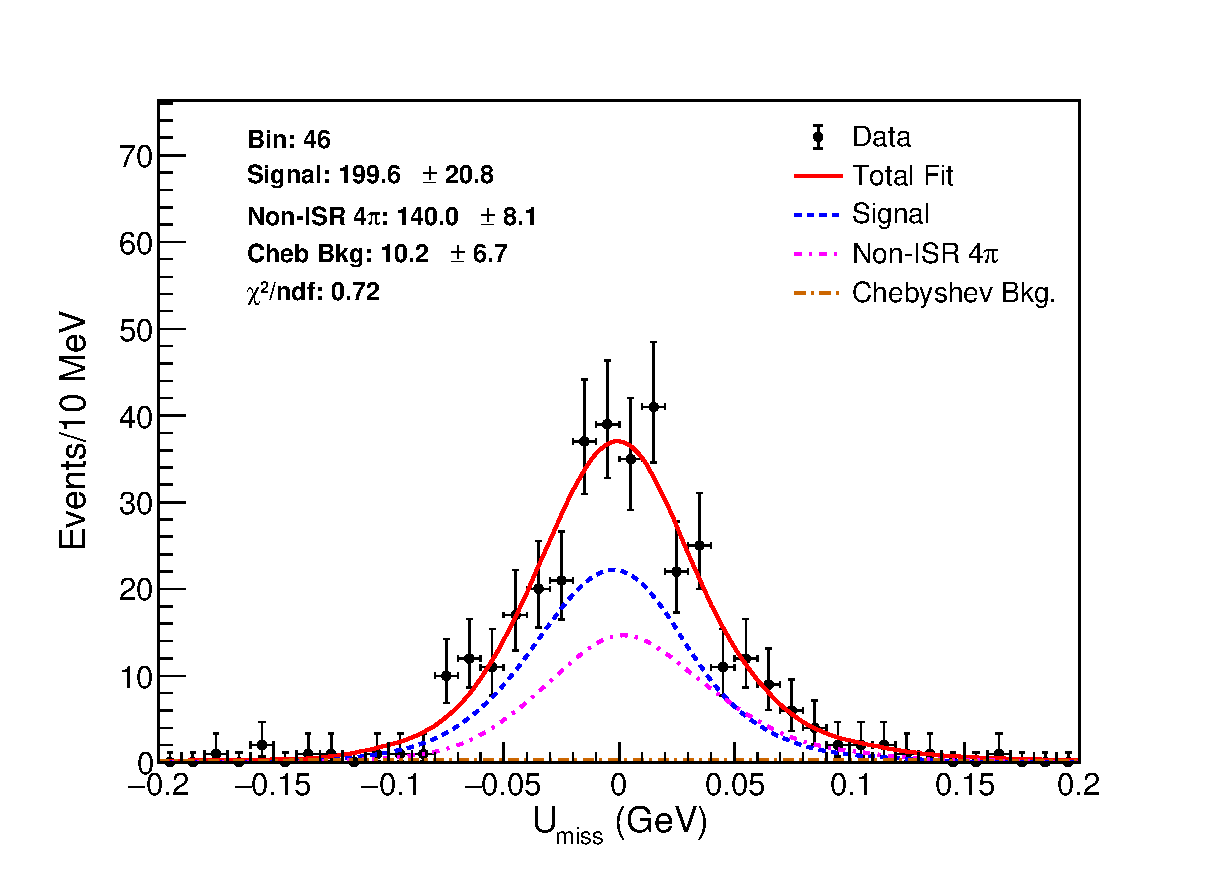
\includegraphics[width=0.32\textwidth]{fig/fit_example_high.eps}
        \label{fig:fit_example_high}
    }
    \caption{Typical $U_{\text{miss}}$ fit results for representative $M_{3\pi}$ bins from each of the three mass regions, shown for Round 16 data.}
    \label{fig:fit_examples}
\end{figure}

Applying this fitting procedure to all $M_{3\pi}$ bins yields the extracted signal yields across the entire mass spectrum. The same fit is performed independently for four data-taking periods: Round~03/04, Round~15, Round~16, and Round~17. Figure~\ref{fig:signal_yields} presents the measured signal yields as a function of $M_{3\pi}$ for all four periods, organized by the three mass regions. In each panel, the $\omega(782)$ resonance is clearly visible as a prominent peak around $0.78~\text{GeV}/c^{2}$, while the $\phi(1020)$ resonance appears as a distinct but smaller peak near $1.02~\text{GeV}/c^{2}$. In the higher mass regions, broad structures corresponding to the $\omega^{\prime}$ and $\omega^{\prime\prime}$ excitations are observed, with significantly reduced yields due to the decreasing cross section and lower ISR photon probability at larger momentum transfers. The results show good consistency across the four data-taking periods, with statistical uncertainties represented by the error bars.

\begin{figure}[htbp]
\centering

% === Row 1: Round 03/04 ===
\subfloat[Round 03/04, $\omega(782)$ region]{
    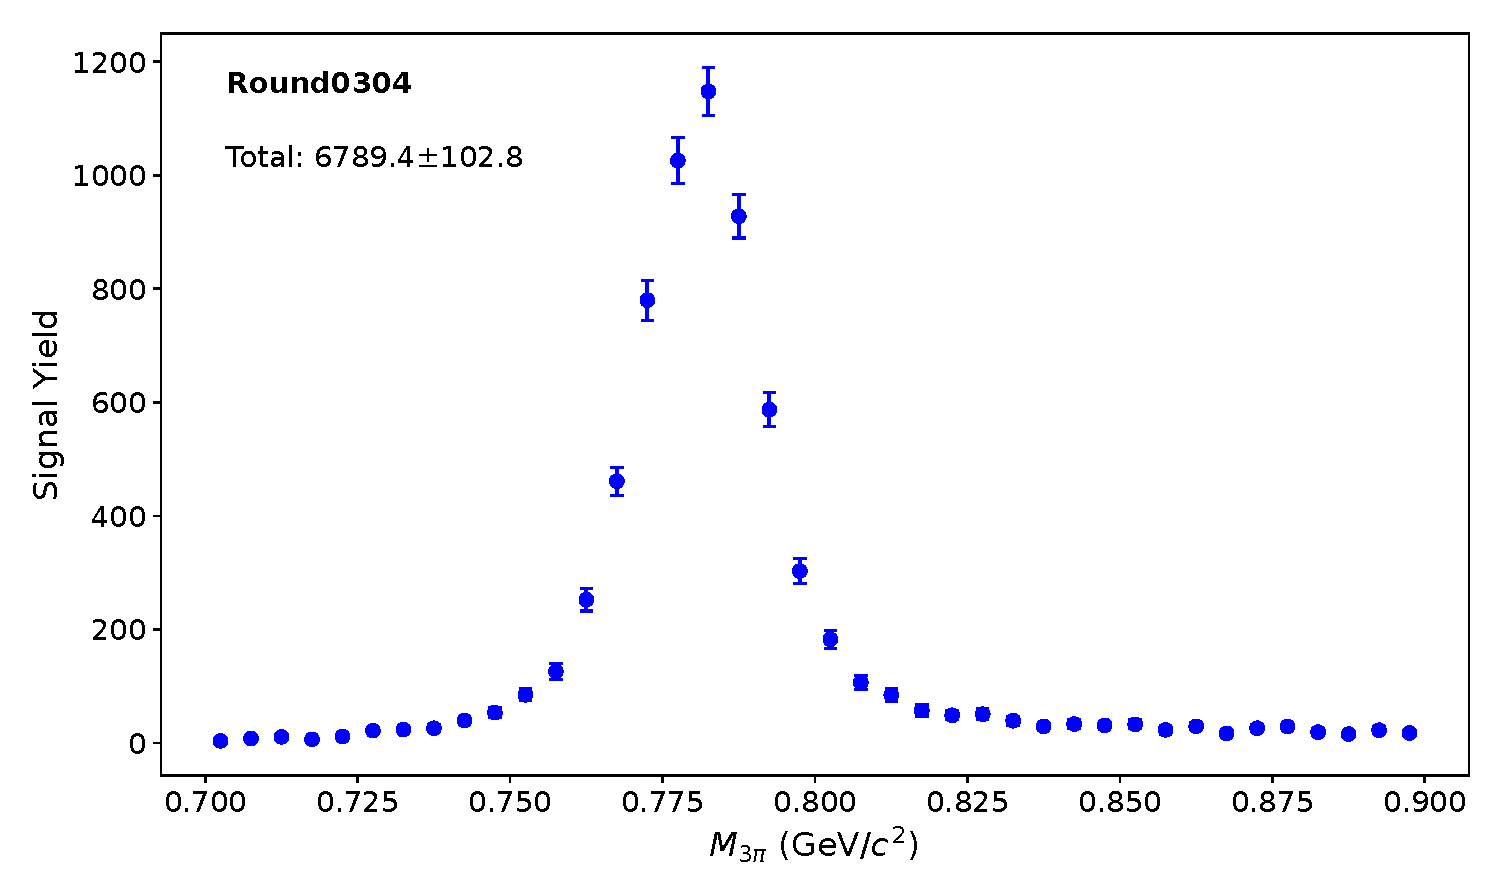
\includegraphics[width=0.32\textwidth]{fig/yields_round0304_region1.eps}
    \label{fig:yields_r0304_region1}
}\hfill
\subfloat[Round 03/04, $\phi(1020)$ region]{
    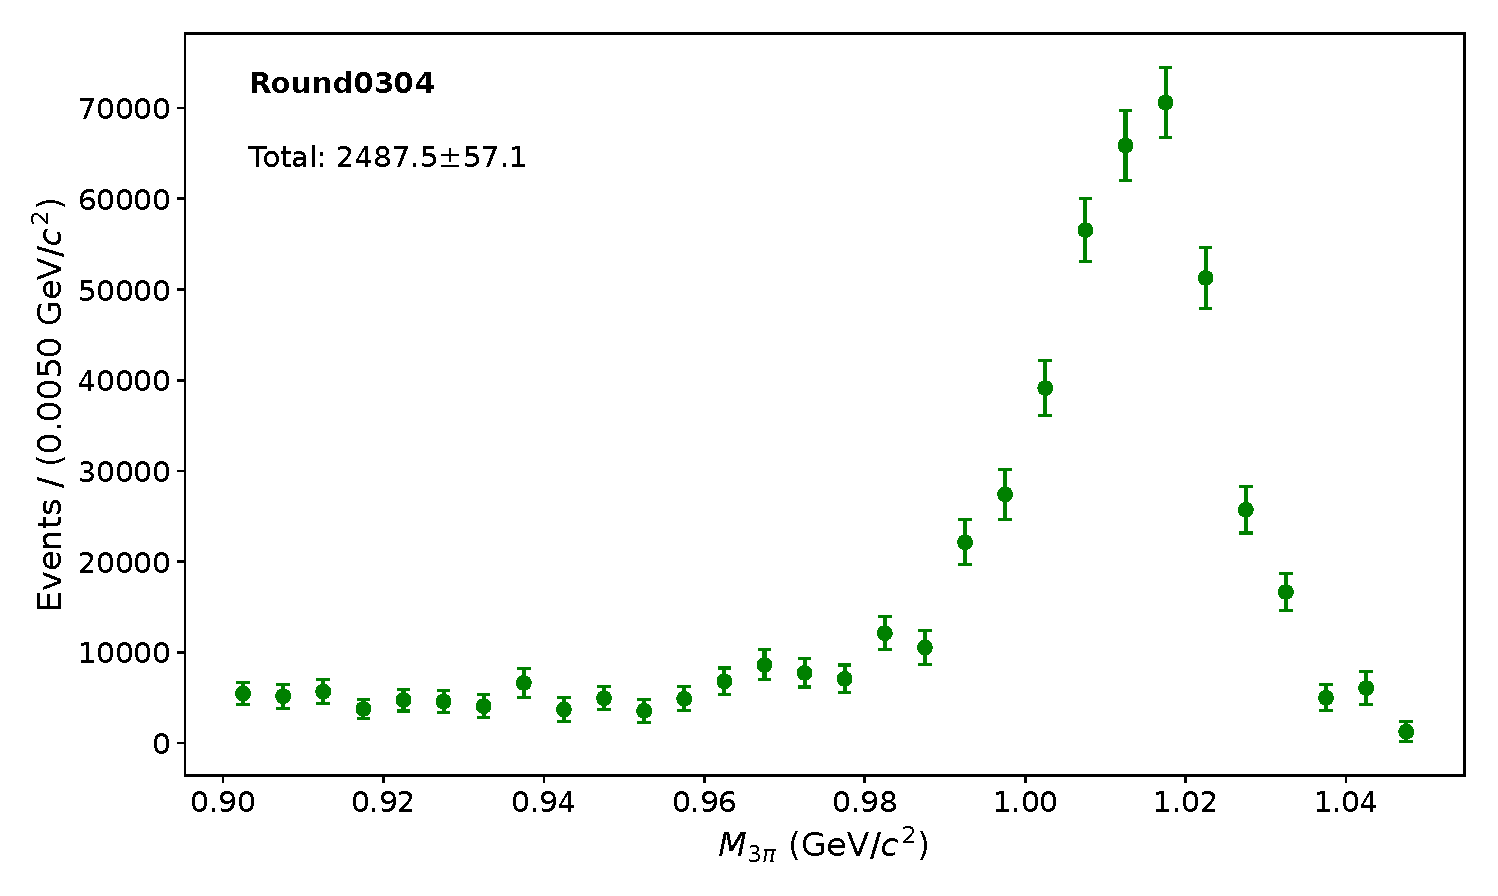
\includegraphics[width=0.32\textwidth]{fig/yields_round0304_region2.eps}
    \label{fig:yields_r0304_region2}
}\hfill
\subfloat[Round 03/04, $\omega^{\prime}/\omega^{\prime\prime}$ region]{
    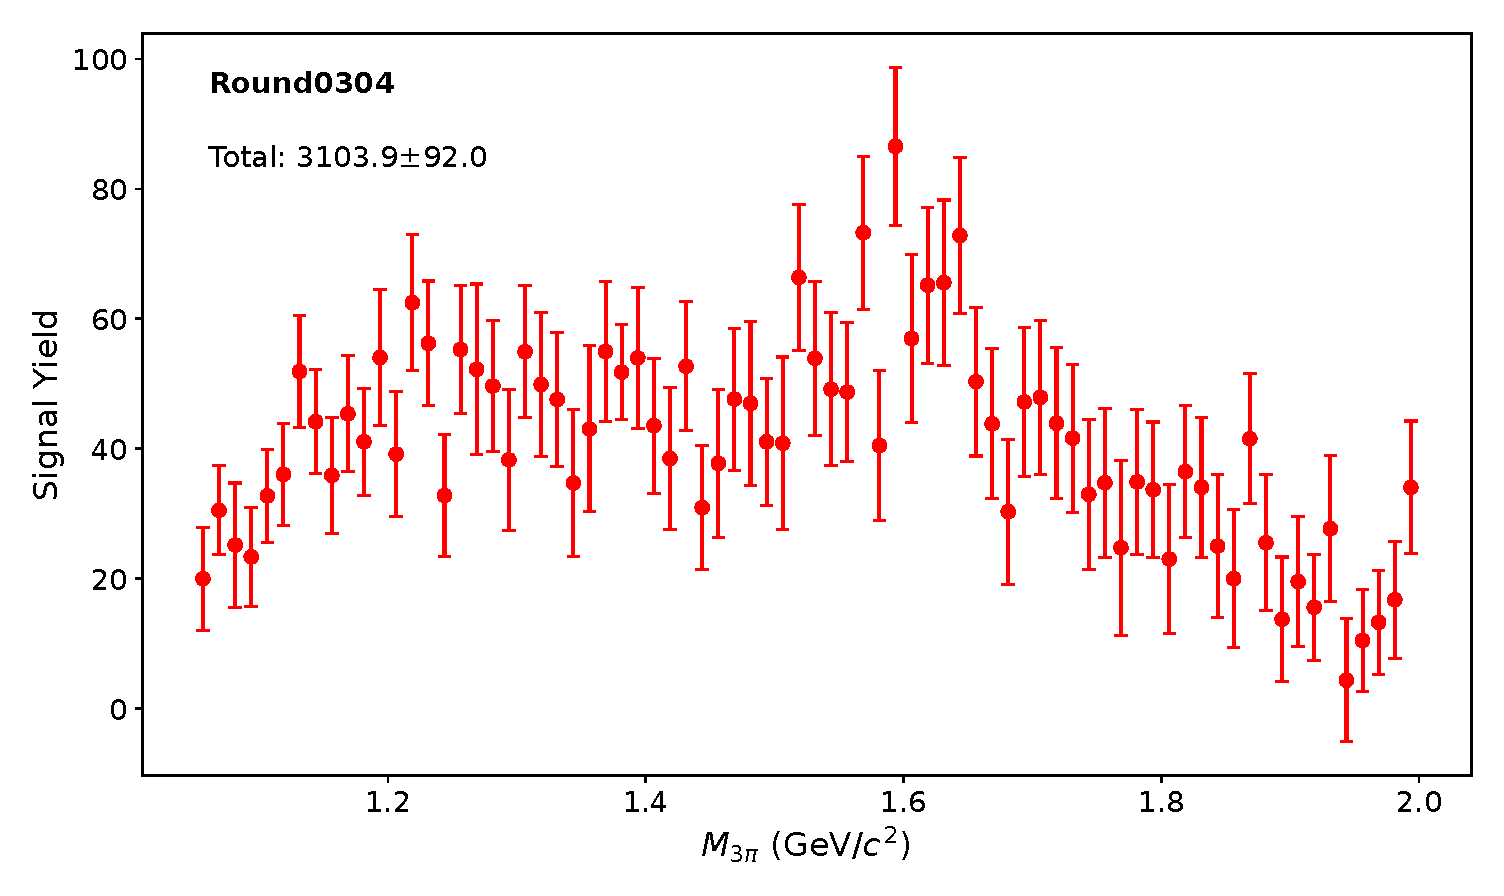
\includegraphics[width=0.32\textwidth]{fig/yields_round0304_region3.eps}
    \label{fig:yields_r0304_region3}
}

\vspace{0.5\baselineskip}

% === Row 2: Round 15 ===
\subfloat[Round 15, $\omega(782)$ region]{
    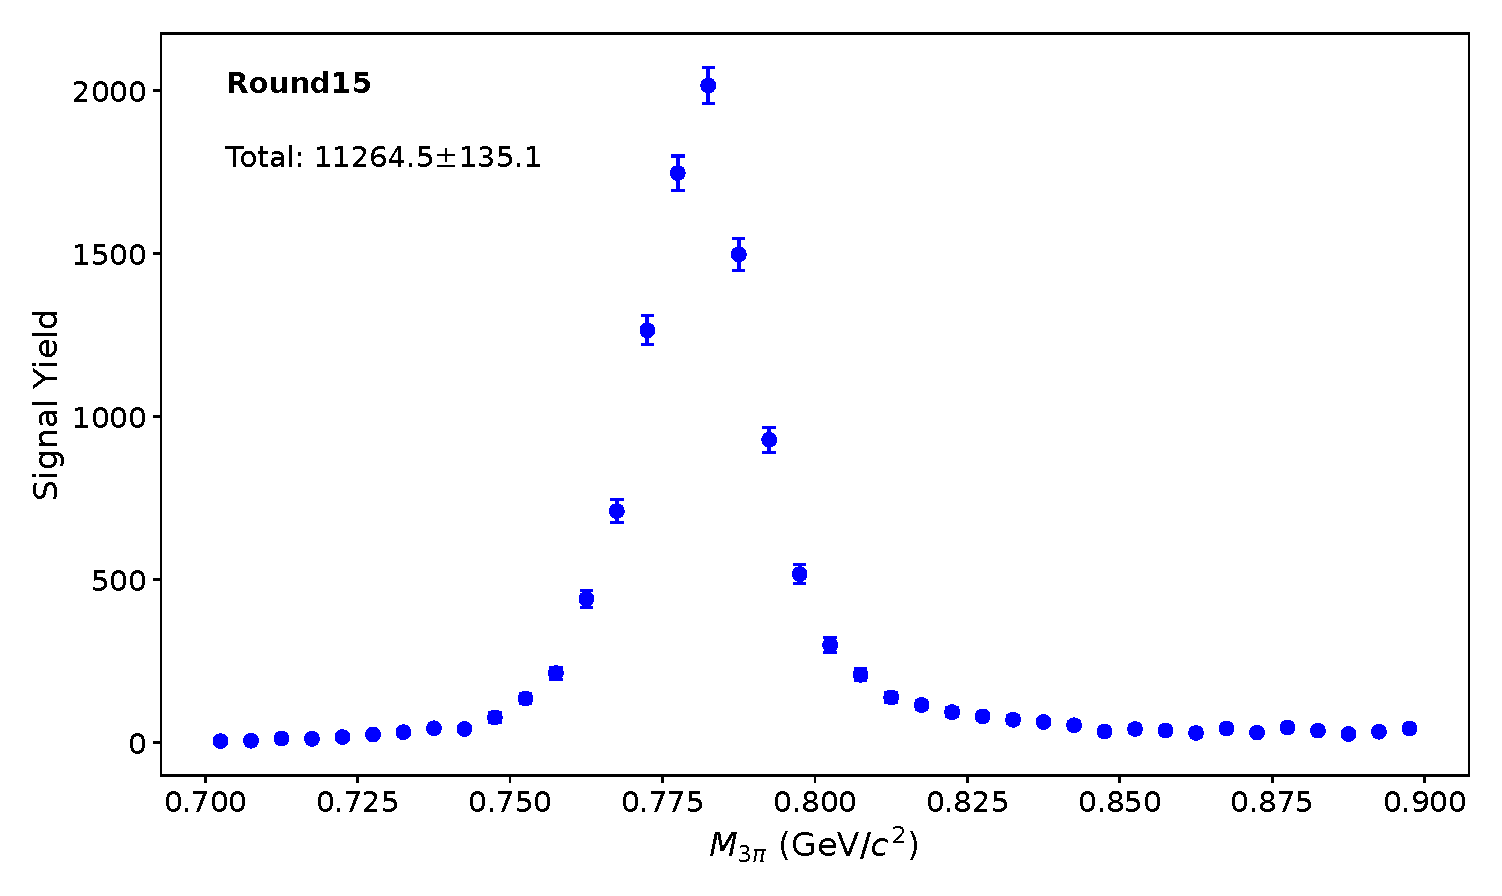
\includegraphics[width=0.32\textwidth]{fig/yields_round15_region1.eps}
    \label{fig:yields_r15_region1}
}\hfill
\subfloat[Round 15, $\phi(1020)$ region]{
    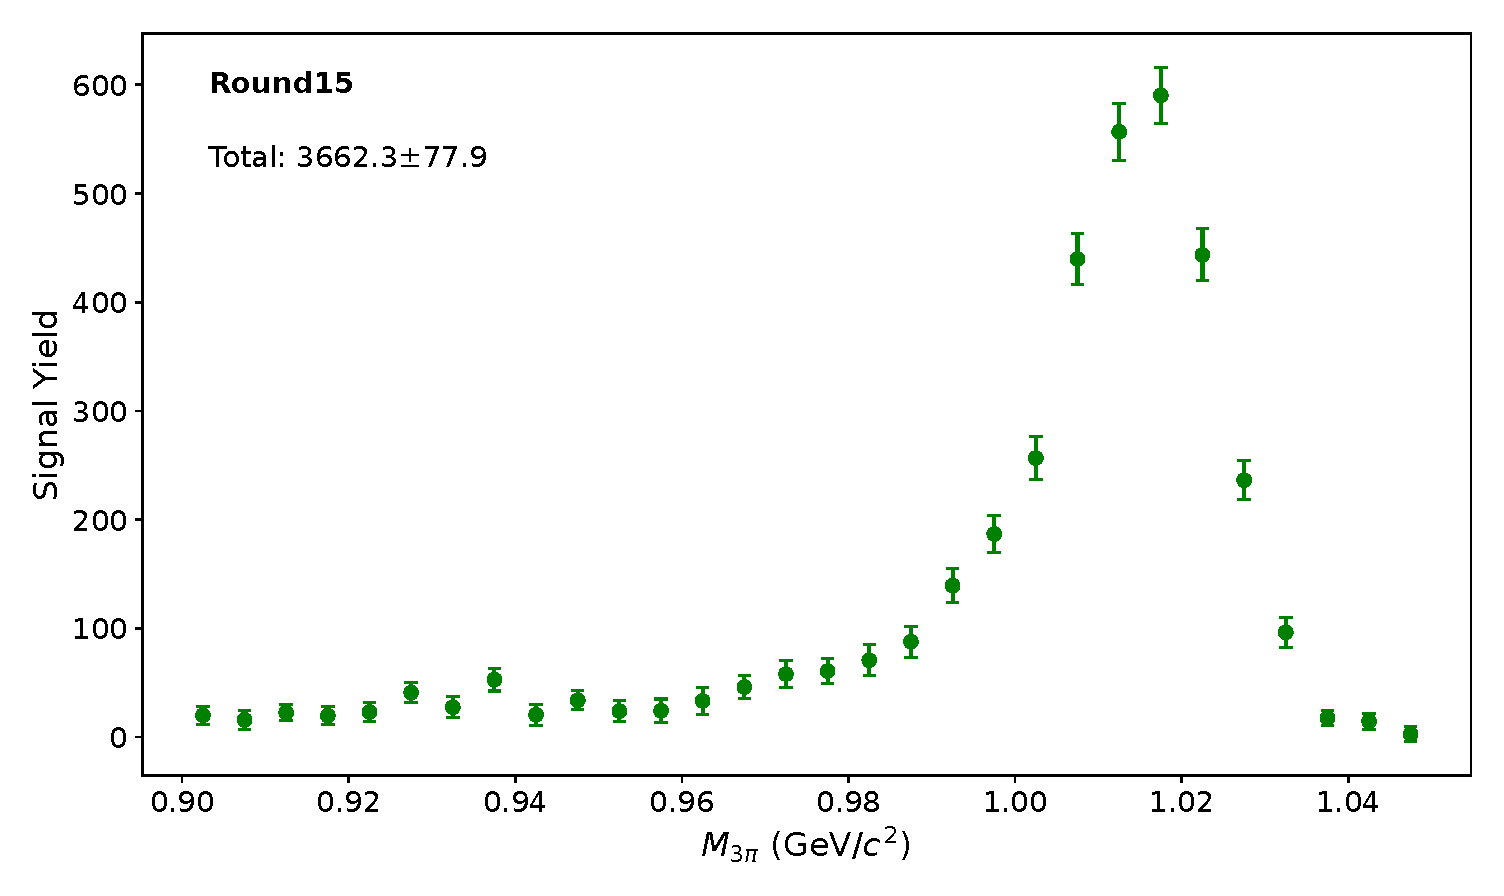
\includegraphics[width=0.32\textwidth]{fig/yields_round15_region2.eps}
    \label{fig:yields_r15_region2}
}\hfill
\subfloat[Round 15, $\omega^{\prime}/\omega^{\prime\prime}$ region]{
    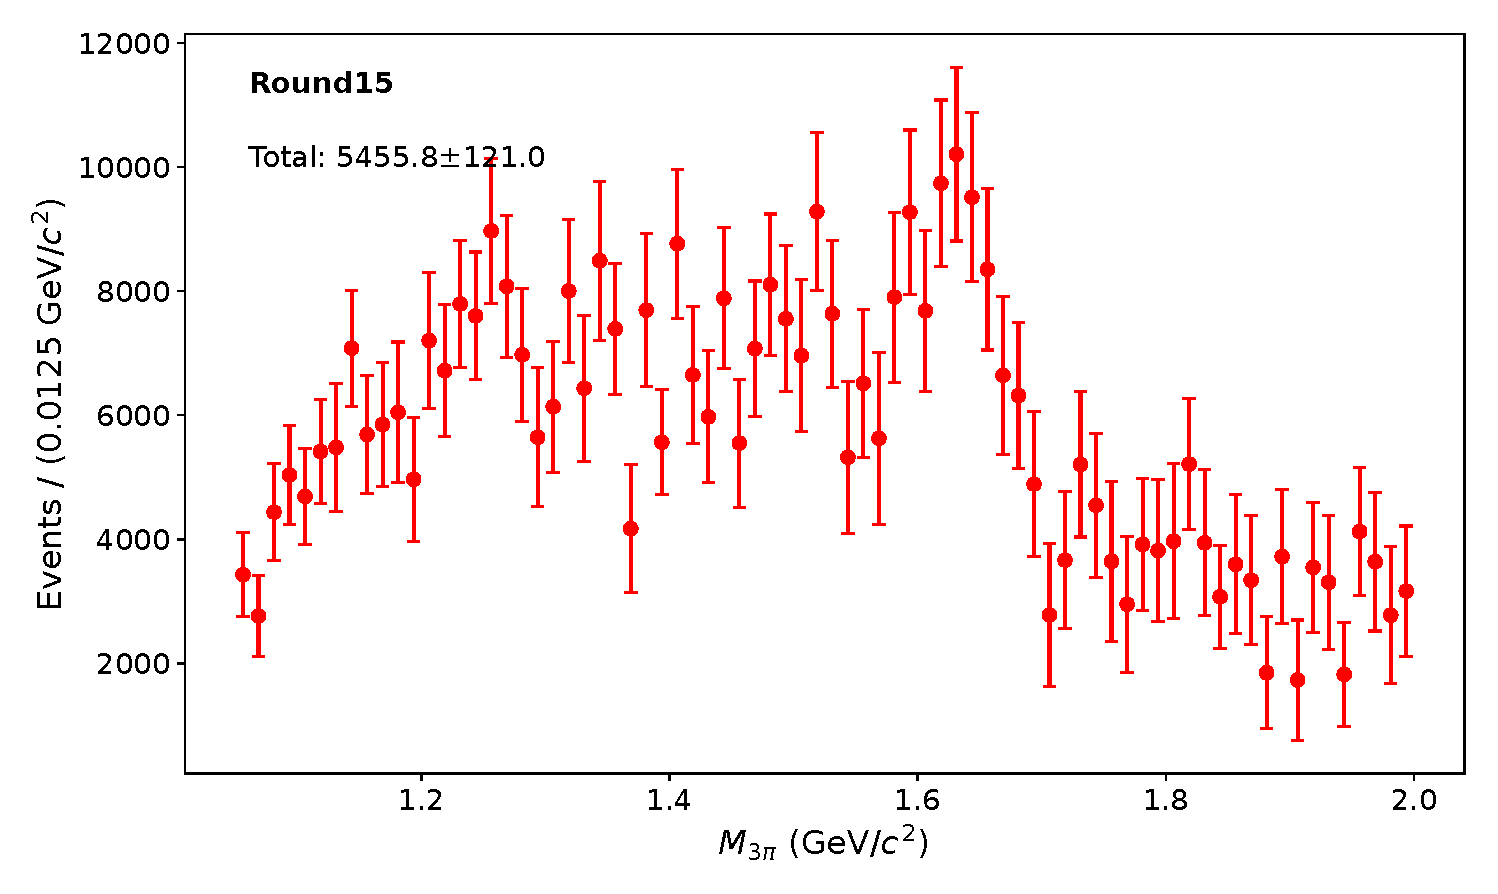
\includegraphics[width=0.32\textwidth]{fig/yields_round15_region3.eps}
    \label{fig:yields_r15_region3}
}

\vspace{0.5\baselineskip}

% === Row 3: Round 16 ===
\subfloat[Round 16, $\omega(782)$ region]{
    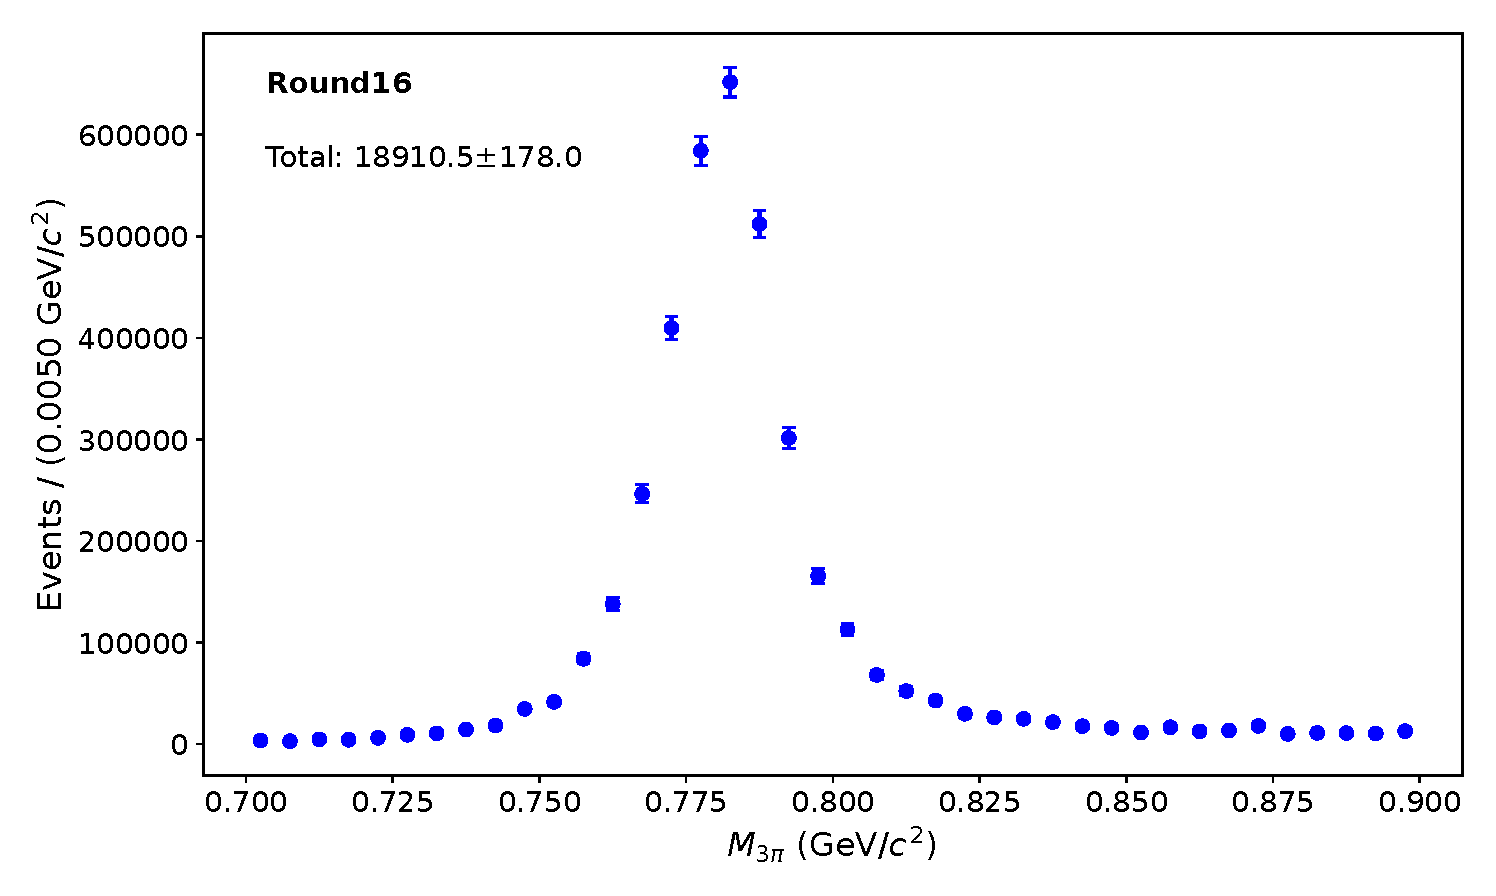
\includegraphics[width=0.32\textwidth]{fig/yields_round16_region1.eps}
    \label{fig:yields_r16_region1}
}\hfill
\subfloat[Round 16, $\phi(1020)$ region]{
    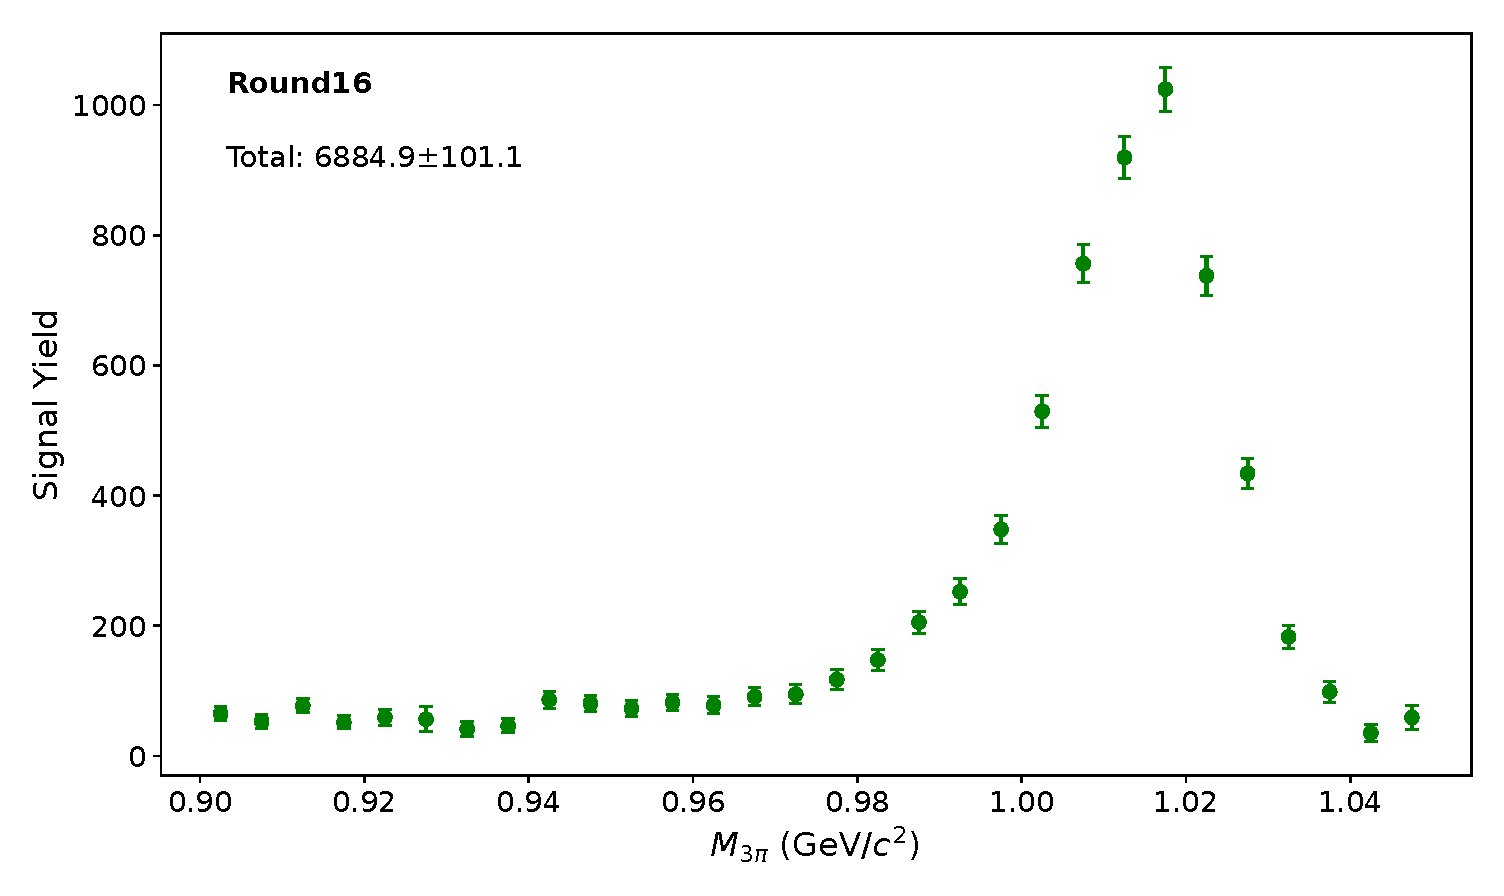
\includegraphics[width=0.32\textwidth]{fig/yields_round16_region2.eps}
    \label{fig:yields_r16_region2}
}\hfill
\subfloat[Round 16, $\omega^{\prime}/\omega^{\prime\prime}$ region]{
    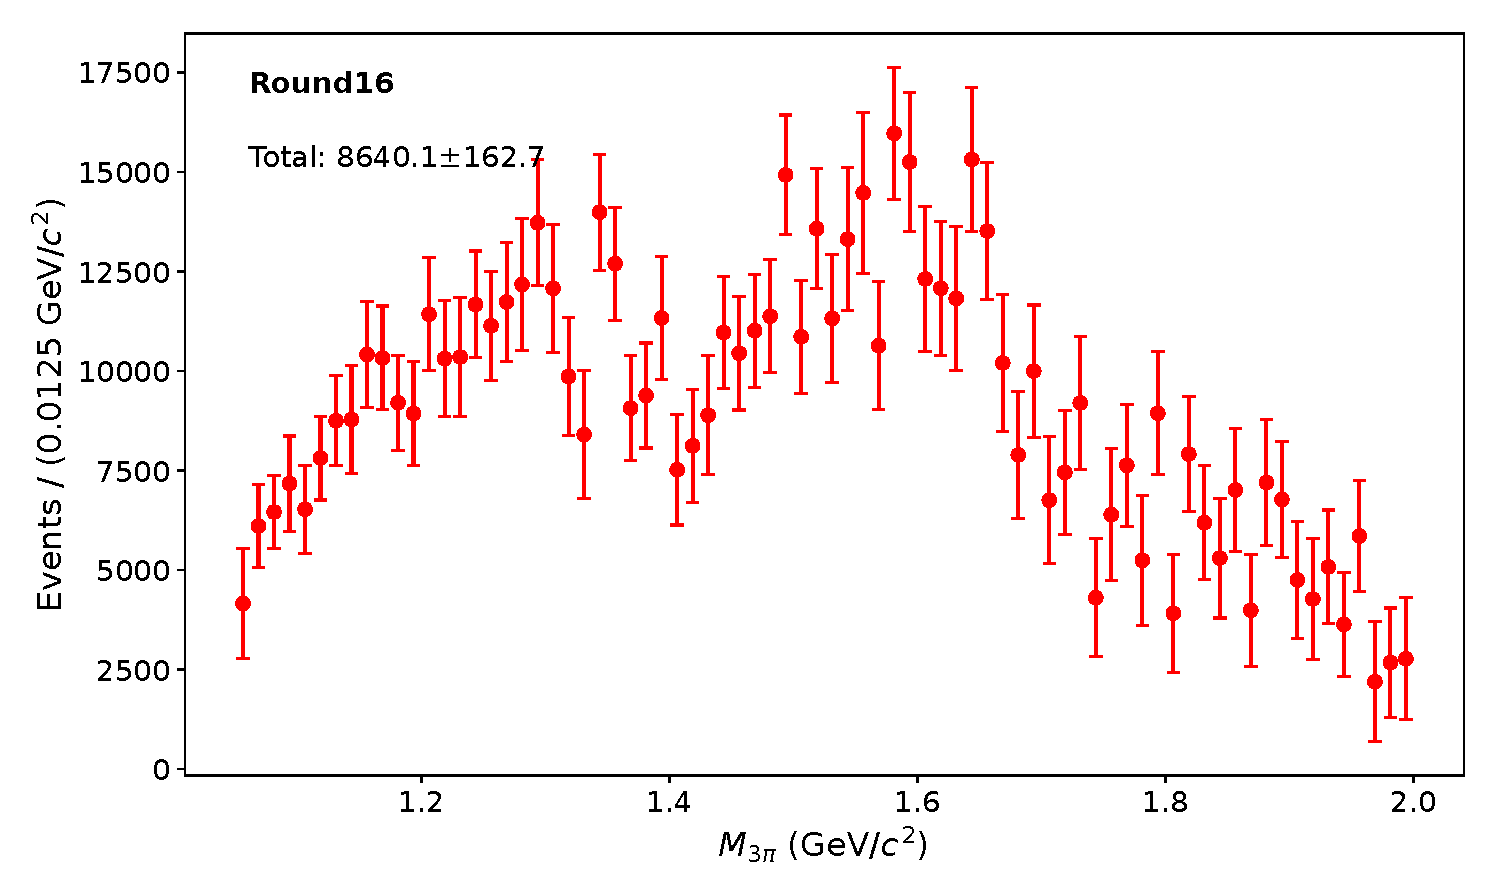
\includegraphics[width=0.32\textwidth]{fig/yields_round16_region3.eps}
    \label{fig:yields_r16_region3}
}

\vspace{0.5\baselineskip}

% === Row 4: Round 17 ===
\subfloat[Round 17, $\omega(782)$ region]{
    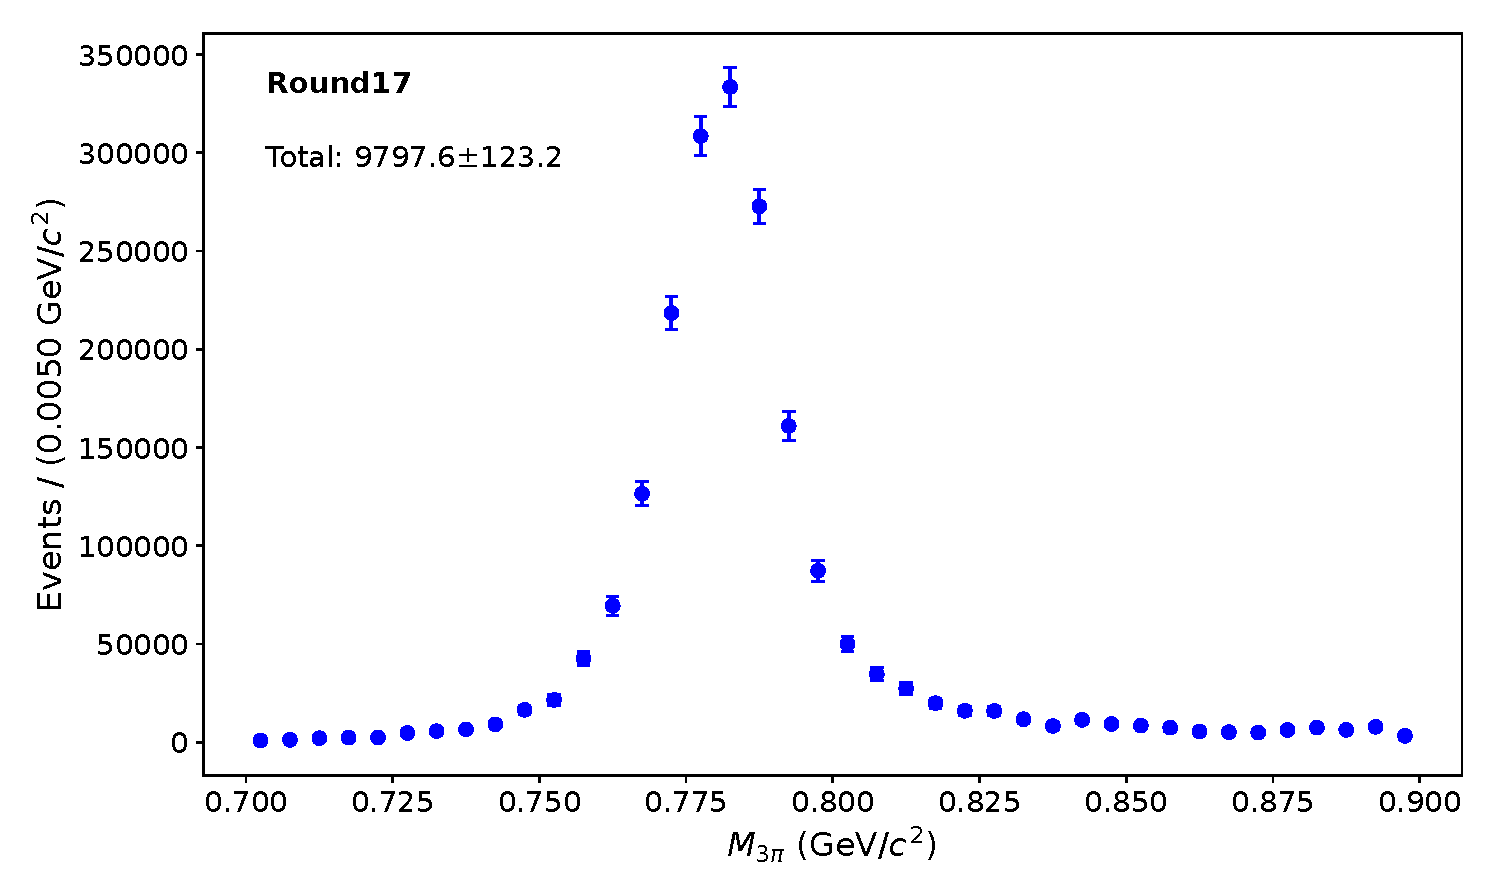
\includegraphics[width=0.32\textwidth]{fig/yields_round17_region1.eps}
    \label{fig:yields_r17_region1}
}\hfill
\subfloat[Round 17, $\phi(1020)$ region]{
    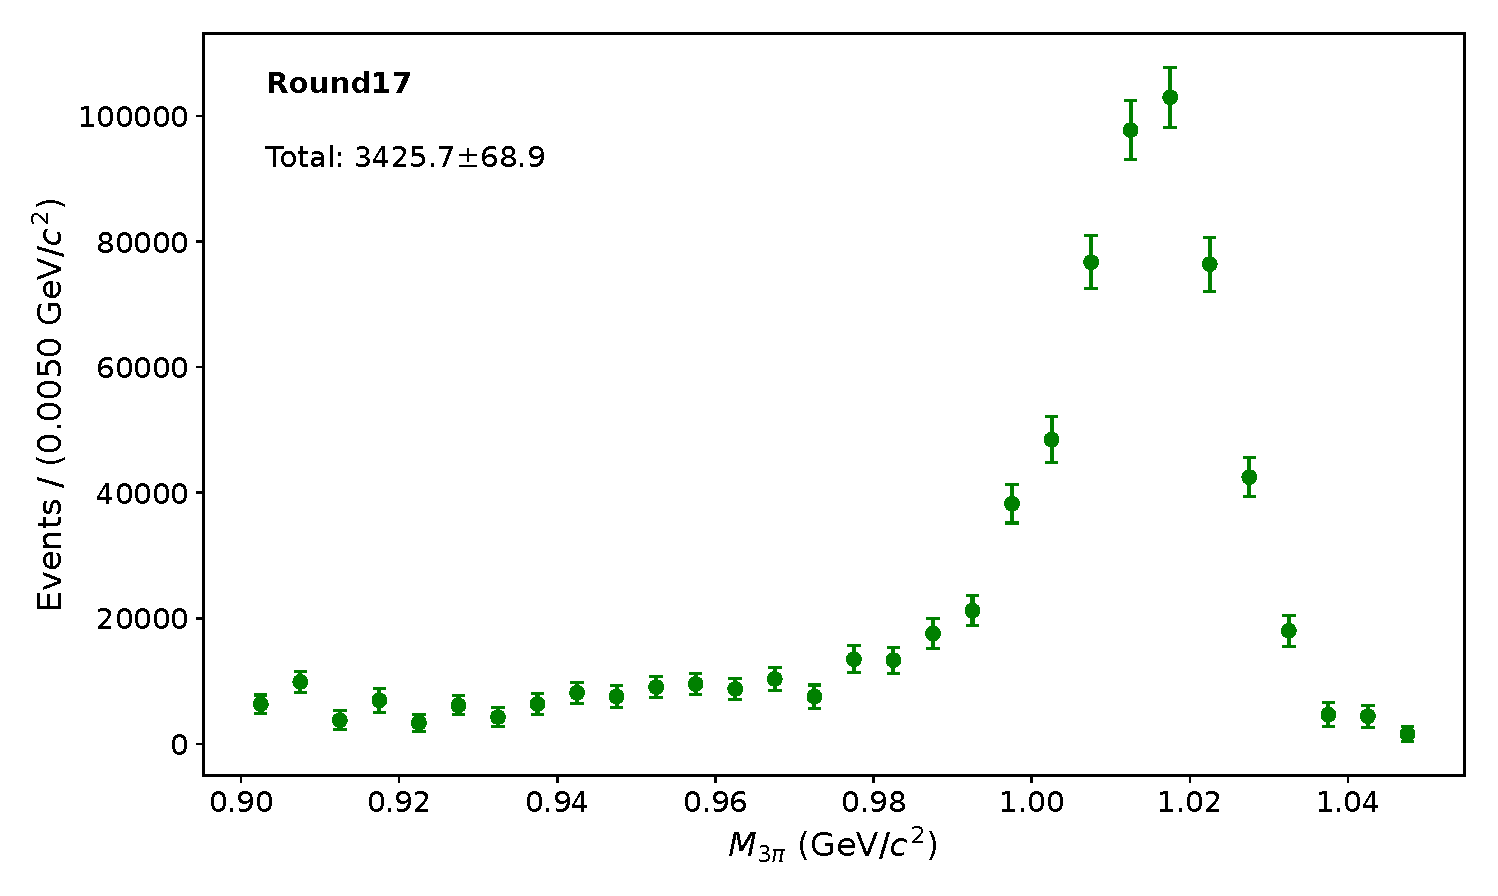
\includegraphics[width=0.32\textwidth]{fig/yields_round17_region2.eps}
    \label{fig:yields_r17_region2}
}\hfill
\subfloat[Round 17, $\omega^{\prime}/\omega^{\prime\prime}$ region]{
    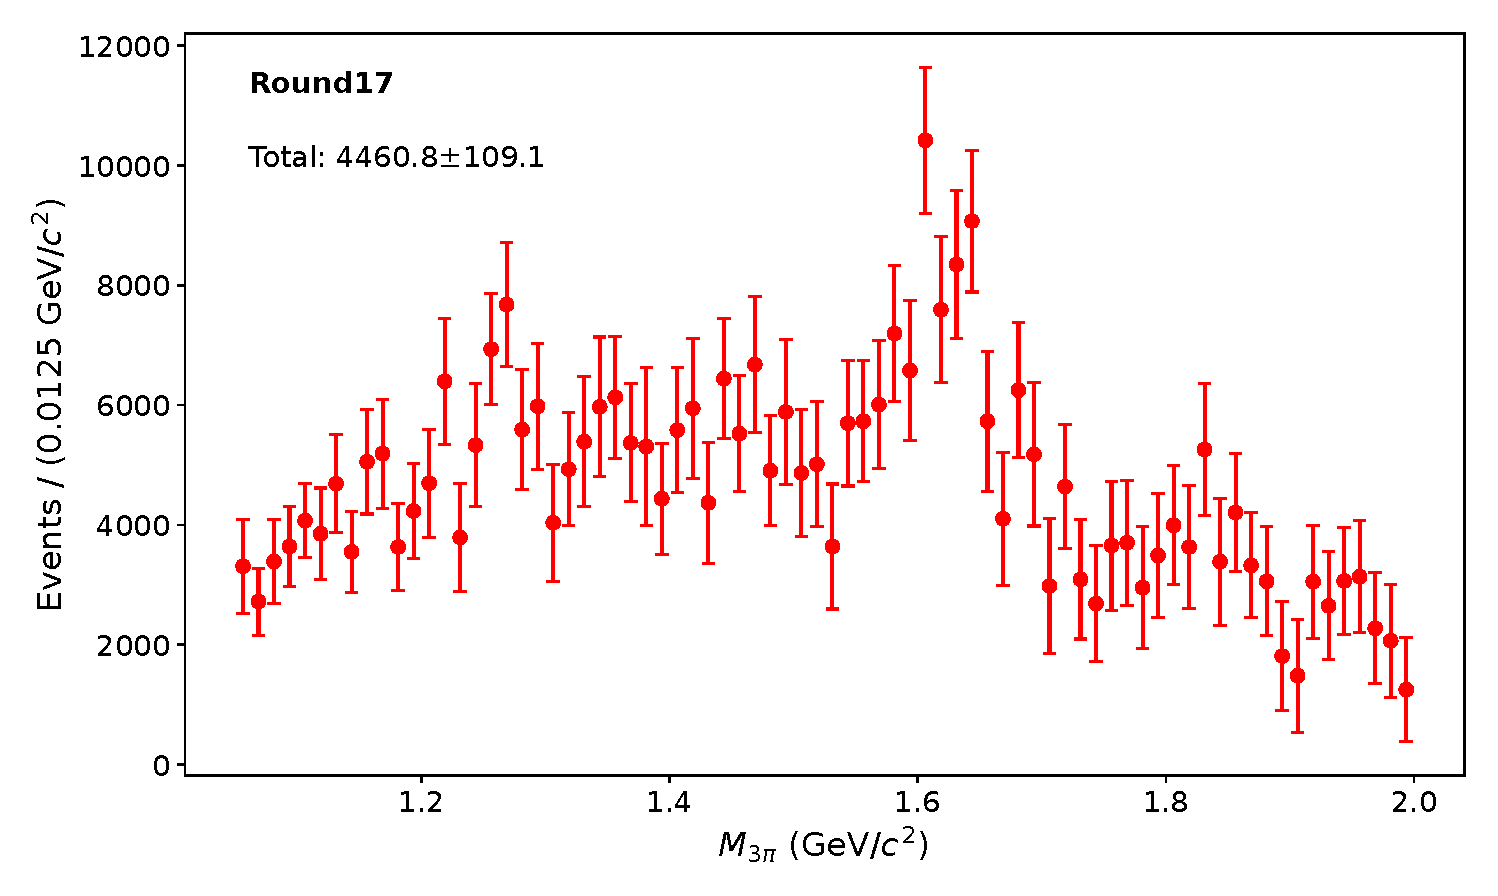
\includegraphics[width=0.32\textwidth]{fig/yields_round17_region3.eps}
    \label{fig:yields_r17_region3}
}

\caption{Extracted signal yields as a function of $M_{3\pi}$ for the three mass regions, shown separately for four data-taking periods. Each row corresponds to a different round: (a)--(c) Round~03/04, (d)--(f) Round~15, (g)--(i) Round~16, and (j)--(l) Round~17. The three columns represent different $3\pi$ invariant mass regions: $\omega(782)$ region (left), $\phi(1020)$ region (center), and higher-mass $\omega^{\prime}/\omega^{\prime\prime}$ region (right). Error bars represent the statistical uncertainties from the fits.}
\label{fig:signal_yields}
\end{figure}

% The signal yields obtained from this fitting procedure provide the foundation for calculating the Born cross section for $e^{+}e^{-} \to \pi^{+}\pi^{-}\pi^{0}$ as a function of $M_{3\pi}$. After applying efficiency corrections, unfolding for resolution effects, and subtracting residual background contributions, the cross section will be determined and compared with previous measurements and theoretical predictions.

% The fit results for the same three representative $M_{3\pi}$ bins are shown in Fig.~\ref{fig:fit_result_examples}, demonstrating the performance of the fitting procedure.

% \begin{figure}[htbp]
%     \centering
%     \subfloat[Low $M_{3\pi}$ bin fit result]{
%         \includegraphics[width=0.32\textwidth]{fig/fit_result_bin_low.eps}
%         \label{fig:fit_low}
%     }
%     \hfill
%     \subfloat[Medium $M_{3\pi}$ bin fit result]{
%         \includegraphics[width=0.32\textwidth]{fig/fit_result_bin_medium.eps}
%         \label{fig:fit_medium}
%     }
%     \hfill
%     \subfloat[High $M_{3\pi}$ bin fit result]{
%         \includegraphics[width=0.32\textwidth]{fig/fit_result_bin_high.eps}
%         \label{fig:fit_high}
%     }
%     \caption{Fit results to the $U_{\text{miss}}$ distributions for the same three representative $M_{3\pi}$ bins as in Fig.~\ref{fig:inclusiveMC_umiss_examples}. Data points are shown with error bars, while the solid black line represents the total fit. The individual components are displayed with the same color scheme as in Fig.~\ref{fig:inclusiveMC_umiss_examples}.}
%     \label{fig:fit_result_examples}
% \end{figure}

% The signal yields extracted from the fits in all $M_{3\pi}$ bins are then combined to form the signal mass spectra for each of the three regions. These spectra, showing the signal yield as a function of $M_{3\pi}$, are presented in Fig.~\ref{fig:signal_yield_spectra}.

% \begin{figure}[htbp]
%     \centering
%     \subfloat[$\omega(782)$ region]{
%         \includegraphics[width=0.32\textwidth]{fig/signal_yield_omega.eps}
%         \label{fig:signal_yield_omega}
%     }
%     \hfill
%     \subfloat[$\phi(1020)$ region]{
%         \includegraphics[width=0.32\textwidth]{fig/signal_yield_phi.eps}
%         \label{fig:signal_yield_phi}
%     }
%     \hfill
%     \subfloat[$\omega^{\prime}/\omega^{\prime\prime}$ region]{
%         \includegraphics[width=0.32\textwidth]{fig/signal_yield_omegaprime.eps}
%         \label{fig:signal_yield_omegaprime}
%     }
%     \caption{Extracted signal yields as a function of $M_{3\pi}$ for (a) the $\omega(782)$ region, (b) the $\phi(1020)$ region, and (c) the $\omega^{\prime}/\omega^{\prime\prime}$ region. The yields are obtained from the extended unbinned maximum-likelihood fits to the $U_{\text{miss}}$ distributions in each $M_{3\pi}$ bin.}
%     \label{fig:signal_yield_spectra}
% \end{figure}